

\chapter{Modular Functions and Algebraic Number Theory}\label{chap3}

\section{Abelian functions and complex
  multiplications}\label{chap3:sec1}\pageoriginale

In this section, we shall see how the complex multiplications of
abelian functions lead in a natural fashion to the study of the
Hilbert modular group.

Let $z_{1},\ldots,z_{n}$ be $n$ independent complex variables and let
$$
z=
\begin{pmatrix}
z_{1}\\
\vdots\\
z_{n}
\end{pmatrix}
$$
Let $C^{n}$ be the $n$-dimensional complex euclidean space and $G$, a
domain in $C^{n}$. A complex-valued function $f(z)$ defined on $G$
(except, perhaps, for a lower-dimensional subset of $G$) is {\em
  meromorphic} in $G$, if there exists a correspondence
$$
a=
\begin{pmatrix}
a_{1}\\
\vdots\\
a_{n}
\end{pmatrix}
(\in G)\to \frac{p_{a}(z)}{q_{a}(z)}
$$
where $p_{a}(z)$ and $q_{a}(z)$ are convergent power-series in
$z_{1}-a_{1},\ldots z_{n}-a_{n}$ with a common domain of convergence
$K_{a}$ around $a$ such that for $z\in K_{a}$,
$f(z)=\dfrac{p_{a}(z)}{q_{a}(z)}$ whenever either $q_{a}(z)\neq 0$ or
if $q_{a}(z)=0$, the $p_{a}(z)\neq 0$.

Let $f(z)$ be a meromorphic function of $z$ in $C^{n}$. A complex
column
$p=\left(\begin{smallmatrix}p_{1}\\\vdots\\ p_{n}
\end{smallmatrix}\right)$ is a {\em period} of $f(z)$, if
$f(z+p)=f(z)$ for all $z\in C^{n}$; for example,
$0=\left(\begin{smallmatrix} 0\\ \vdots\\ 0
\end{smallmatrix}\right)$ is a period of $f(z)$. The periods of $f(z)$
form an additive\pageoriginale abelian group; if we regard $C^{n}$ as
a $2n$-dimensional real vector space, then the group of periods is, in
fact, a closed vector group over the field of real numbers. Either
this vector group is discrete or it contains at least one limit point
in $C^{n}$. In the latter case, $f(z)$ is said to be {\em degenerate};
this is equivalent to the fact that $f(z)$ has infinitesimal periods
and by a suitable linear transformation of the variables
$z_{1},\ldots,z_{n}$ with complex coefficients, the function $f(z)$
can be brought to depend on strictly less than $n$ complex
variables. In the former case, $f(z)$ is said to be {\em
  non-degenerate} and its period-group is a discrete vector-group \ie
a lattice in $C^{n}$. We shall consider only the case when the
period-lattice has $2n$ generators linearly independent over the field
of real numbers. It is easy to construct an example of a
non-degenerate abelian function with $2n$ independent periods. For
example, let $\mathscr{P}(w)$ be the Weierstrass' elliptic function
with independent periods $\omega_{1}$, $\omega_{2}$. Then the function
$f(z)=\mathscr{P}(z_{1})\ldots\mathscr{P}(z_{n})$ furnishes the
required example, since it has exactly $2n$ independent periods
$$
\begin{pmatrix}
\omega_{1}\\
\cdot\\
\cdot\\
0\\
0
\end{pmatrix},
\begin{pmatrix}
\omega_{2}\\
\cdot\\
\cdot\\
0\\
0
\end{pmatrix},
\begin{pmatrix}
0\\
\omega_{1}\\
0\\
\cdot\\
0
\end{pmatrix},
\begin{pmatrix}
0\\
\omega_{2}\\
0\\
\cdot\\
0
\end{pmatrix},\ldots,
\begin{pmatrix}
0\\
\cdot\\
\cdot\\
0\\
\omega_{1}
\end{pmatrix},
\begin{pmatrix}
0\\
\cdot\\
\cdot\\
0\\
\omega_{2}
\end{pmatrix}.
$$

Let, then, for a given $f(z)$ meromorphic in $C^{n}$,
$p_{1},\ldots,p_{2n}$ be $2n$ periods linearly independent over the
field of real numbers such that any period $p$ of $f(z)$ is of the
form $\sum^{2n}_{i=1}m_{i}p_{i}$ with rational integers $m_{i}$. The
$n$-rowed matrix $P=(p_{1},\ldots,p_{2n})$ is called a {\bf
  period-matrix} of $f(z)$. It is uniquely determined upto
multiplication on the right by a $2n$-rowed unimodular matrix. We
shall denote the period-lattice generated by $p_{1},\ldots,p_{2n}$ in
$C^{n}$ by $\mathfrak{L}$.

A meromorphic function $f(z)$ defined in $C^{n}$ and admitting as
periods all the elements of $\mathfrak{L}$ is called an {\bf abelian
  function for the lattice} $\mathfrak{L}$. The abelian functions for
$\mathfrak{L}$ constitute a field $\mathfrak{F}_{\mathfrak{L}}$. In
$\mathfrak{F}_{\mathfrak{L}}$ there exists at least one function
$f(z)$ having $\mathfrak{L}$ exactly as its period-lattice. Moreover,
in $\mathfrak{F}_{\mathfrak{L}}$, there exist $n$ functions
$f_{1},\ldots,f_{n}$ which are analytically independent and hence
algebraically independent over the field of complex
numbers. Also,\pageoriginale every abelian function satisfies a
polynomial equation of bounded degree with rational functions of
$f_{1},\ldots,f_{n}$ as coefficients. As a consequence, it can be
shown that $\mathfrak{F}_{\mathfrak{L}}$ is an algebraic function
field of $n$ variables and one can find $n+1$ functions, $f_{0}$,
$f_{1},\ldots,f_{n}$ in $\mathfrak{F}_{\mathfrak{L}}$ such that every
function in $\mathfrak{F}_{\mathfrak{L}}$ is a rational function of
$f_{0}$, $f_{1},\ldots,f_{n}$ with complex coefficients.

Let $P$ be a complex matrix of $n$ rows and $2n$ columns such that the
$2n$ columns are linearly independent over the field of real
numbers. The problem arises as to when $P$ is a period-matrix of a
non-degenerate abelian function or, in other words, a {\bf Riemann
  matrix}. It is well known that in order that $P$ might be a Riemann
matrix, it is necessary and sufficient that there exists a rational
$2n$-rowed alternate (skew-symmetric) matrix $A$ such that
\begin{equation*}
\begin{aligned}
& {\rm (i)}~ PAP'=0,\\
& {\rm (ii)}~ H=i^{-1}\ob{P}AP'>0 \text{ (\ie positive hermitian).}
\end{aligned}\tag{133}\label{133}
\end{equation*}
These are known as the {\em period relations.} If $E$ is the $n$-rowed
identity matrix and $A$ is the $2n$-rowed alternate matrix
$\left(\begin{smallmatrix} 0 & E\\ -E & 0
\end{smallmatrix}\right)$, then conditions (i) and (ii) were given by
Riemann as precisely the conditions to be satisfied by the periods of
a normalised complete system of abelian integrals of the first kind on
a Riemann surface of genus $n$.

Setting $B=\left(\dfrac{P}{P}\right)$, the two conditions above may be
written in the form
\begin{equation*}
BAB'=
\begin{pmatrix}
0 & -i\ob{H}\\
iH & 0
\end{pmatrix},\quad H>0.\tag{134}\label{134}
\end{equation*}
For $n=1$, the conditions \eqref{133} reduce to the sole condition
that if $P=(\omega_{1}\omega_{2})$, then $\omega_{1}\omega^{-1}_{2}$
should not be real. To establish the necessity and sufficiency of
these conditions for $n>1$, one has to make considerable use of
theta-functions.

The problem as to when a given $P$ is a Riemann matrix was apparently
considered independently also by Weierstrass and he wished to prove to
this end that every abelian function can be written as the quotient of
two theta-functions. He could not, however, complete the proof of this
last statement--it\pageoriginale was Appell who gave a complete proof
of the same for $n=2$, and Poincar\'e, for general $n$.

A period matrix $P$ which satisfies the period-relations with respect
to an alternate matrix $A$ is said to be {\em polarized with respect
  to $A$.} The alternate matrix $A$ is not unique; but, in general,
$A$ is uniquely determined upto a positive rational scalar
factor. Moreover, if $P$ is polarized with respect to $A$, then from
\eqref{134}, since $H>0$, we conclude that $|A|\neq 0$, $|B|\neq 0$.

Let $P$ be a Riemann matrix and $\mathfrak{L}$, the associated lattice
in $C^{n}$. Let $\mathfrak{L}_{1}$ be a sublattice of $\mathfrak{L}$,
again of rank $2n$ over the field of real numbers and let $P_{1}$ be a
period matrix of $\mathfrak{L}_{1}$. Then $P_{1}=PR_{1}$ for a
nonsingular rational integral matrix $R_{1}$. The associated function
field $\mathfrak{F}_{\mathfrak{L}_{1}}$ is an algebraic function field
of $n$ variables, containing $\mathfrak{F}_{\mathfrak{L}}$. Since
$\mathfrak{F}_{\mathfrak{L}}$ itself is an algebraic function field of
$n$ variables, we see that $\mathfrak{F}_{\mathfrak{L}_{1}}$ is an
algebraic extension of $\mathfrak{F}_{\mathfrak{L}}$.

Conversely, let $\mathfrak{F}_{\mathfrak{L}_{1}}$ be a field of
abelian functions, $P_{1}$ an associated Riemann matrix and
$\mathfrak{L}_{1}$ the corresponding period-lattice in
$C^{n}$. Further, let $\mathfrak{F}$ be a subfield of
$\mathfrak{F}_{\mathfrak{L}_{1}}$ such that
$\mathfrak{F}_{\mathfrak{L}_{1}}$ is algebraic over
$\mathfrak{F}_{\mathfrak{L}}$. Then $\mathfrak{F}$ is again a field of
abelian functions containing at least one non-degenerate abelian
function and has a period-lattice $\mathfrak{L}$ containing
$\mathfrak{L}_{1}$. This means that if $P$ is a period-matrix
associated with $\mathfrak{F}$, then $P_{1}=PR_{1}$ for a nonsingular
rational integral matrix $R_{1}$. We now prove

\begin{proposition}\label{prop19}
Let $P_{1}$ and $P_{2}$ be two Riemann matrices and $\mathfrak{L}_{1}$
and $\mathfrak{L}_{2}$ the associated period lattices in $C^{n}$. A
necessary and sufficient condition that the elements of
$\mathfrak{F}_{\mathfrak{L}_{1}}$ depend algebraically on those of
$\mathfrak{F}_{\mathfrak{L}_{2}}$ and vice versa, is that $P_{1}=PM$
for a nonsingular rational matrix $M$.
\end{proposition}

\begin{proof}
Let $f_{0},\ldots,f_{n}$ be generators of
$\mathfrak{F}_{\mathfrak{L}_{1}}$ over the field of complex numbers
and let elements of $\mathfrak{F}_{\mathfrak{L}_{1}}$ depend
algebraically on those of $\mathfrak{F}_{\mathfrak{L}_{2}}$. This
means that each $f_{i}$ satisfies an irreducible polynomial equation
$$
f^{n_{i}}_{i}+a^{(i)}_{n_{i}-1}f^{n_{i}-1}_{i}+\cdots+a^{(i)}_{0}=0,
$$
where $a^{(i)}_{m}$, $m=0$, $1,\ldots,n_{i}-1$ belong to
$\mathfrak{F}_{\mathfrak{L}_{2}}$. Moreover, it is easy to see that
$a^{(i)}_{m}$ for $m=0$, $1,\ldots,n_{i}-1$ and $i=0$, $1,\ldots,n$
lie in $\mathfrak{F}_{\mathfrak{L}_{1}}$. Then the field
$\mathfrak{F}_{\mathfrak{L}}$ generated by $\{a^{(i)}_{m}\}$ over the
field of complex numbers is\pageoriginale a field of abelian functions
contained in both $\mathfrak{F}_{\mathfrak{L}_{1}}$ and
$\mathfrak{F}_{\mathfrak{L}_{2}}$ and hence admitting for periods, all
the elements of $\mathfrak{L}_{1}$ and $\mathfrak{L}_{2}$. Since
$\mathfrak{F}_{\mathfrak{L}_{1}}$ is algebraic over
$\mathfrak{F}_{\mathfrak{L}}$, $\mathfrak{F}_{\mathfrak{L}}$ is an
algebraic function field of $n$ variables and hence
$\mathfrak{F}_{\mathfrak{L}_{2}}$ is also algebraic over
$\mathfrak{F}_{\mathfrak{L}}$. Let $P$ be a period matrix of
$\mathfrak{F}_{\mathfrak{L}}$ and $\mathfrak{L}$, the associated
lattice in $C^{n}$. Then $\mathfrak{L}$ contains both
$\mathfrak{L}_{1}$ and $\mathfrak{L}_{2}$. Hence $P_{1}=PR_{1}$ and
$P_{2}=PR_{2}$ for nonsingular rational integral matrices $R_{1}$ and
$R_{2}$. Thus $P_{1}=P_{2}M$ for a nonsingular rational matrix $M$.
\end{proof}

Conversely, if $P_{1}=P_{2}M$ for a nonsingular rational matrix $M$,
then there exists a Riemann matrix $P$ such that $P_{1}=PR_{1}$ and
$P_{2}=PR_{2}$ for nonsingular rational integral matrices $R_{1}$ and
$R_{2}$ respectively. If $\mathfrak{L}$ is the period-lattice in
$C^{n}$ associated with $P$, the field $\mathfrak{F}_{\mathfrak{L}}$
of abelian functions for $\mathfrak{L}$, is contained in both
$\mathfrak{F}_{\mathfrak{L}_{1}}$ and
$\mathfrak{F}_{\mathfrak{L}_{2}}$. Moreover
$\mathfrak{F}_{\mathfrak{L}_{1}}$ and
$\mathfrak{F}_{\mathfrak{L}_{2}}$ are algebraic over
$\mathfrak{F}_{\mathfrak{L}}$. Thus the condition is also sufficient.

Two lattices $\mathfrak{L}_{1}$ and $\mathfrak{L}_{2}$ in $C^{n}$, of
rank $2n$ over the field of real numbers and having $P_{1}$ and
$P_{2}$ for period-matrices respectively are said to be {\em
  commensurable} if there is another lattice $\mathfrak{L}$ of rank
$2n$ containing both $\mathfrak{L}_{1}$ and $\mathfrak{L}_{2}$ or {\em
  equivalently}: $P_{1}=P_{2}M$ for a nonsingular rational matrix
$M$. Thus in Proposition \ref{prop19}, the necessary and sufficient
condition may also be stated that the lattices $\mathfrak{L}_{1}$ and
$\mathfrak{L}_{2}$ associated with $P_{1}$ and $P_{2}$ are
commensurable.

Let $f(z)$ be a non-degenerate abelian function with period matrix $P$
and period lattice $\mathfrak{L}$ and let $m$ be a scalar. The
function $f(mz)$ has period matrix $m^{-1}P$. If $m$ is rational, then
the period lattice associated with $m^{-1}P$ is clearly commensurable
with $\mathfrak{L}$ and hence $f(mz)$ depends algebraically on the
field $\mathfrak{F}_{\mathfrak{L}}$, in view of Proposition
\ref{prop19}. This is the analogue of the well-known {\em
  multiplication theorem} for elliptic functions. We now ask for all
scalars $m$ such that if $f(z)\in\mathfrak{F}_{\mathfrak{L}}$, $f(mz)$
is algebraic over $\mathfrak{F}_{\mathfrak{L}}$. Let us first consider
the case $n=1$.

Let $p_{1}$, $p_{2}$ be two independent periods of an elliptic
function $f(z)$ such that every other period $p$ of $f(z)$ is of the
form $rp_{1}+sp_{2}$ with rational integral $r$ and $s$. In order that
$f(mz)$ be algebraic over the field of elliptic functions with periods
$p_{1}$ and $p_{2}$, it is necessary and sufficient that
$$
m(p_{1}p_{2})=(p_{1}p_{2})
\begin{pmatrix}
a & b\\
c & d 
\end{pmatrix}
$$
with rational $a$, $b$, $c$, $d$. This means that $m$ is the root of a
quadratic equation\pageoriginale with rational coefficients. More
precisely, $m$ should be an imaginary quadratic irrationality lying in
the field $\bQ(p_{2}p^{-1}_{1})$ where $\bQ$ is the field of rational
numbers. If we require that $f(mz)$ should again be an elliptic
function with $p_{1}$ and $p_{2}$ as periods, then $a$, $b$, $c$, $d$
should be rational integers. This was the {\bf principle of complex
  multiplication} for elliptic functions formulated by Abel in his
work, ``Recherches sur les functions elliptiques''. The idea of
complex multiplication in its simplest form, however, appears to be
contained implicitly in the work of Fagnano, concerning the doubling
of an arc of the lemniscate of Bernoulli.

If $f(z)$ is a non-degenerate abelian function with period matrix $P$
and period lattice $\mathfrak{L}$ and $Q$ is an $n$-rowed complex
non-singular matrix, then $f(Q^{-1}z)$ is a non-degenerate abelian
function with period matrix $QP$. We formerly wished to find all
complex numbers $m$ such that for every
$f(z)\in\mathfrak{F}_{\mathfrak{L}}$, $f(mz)$ is algebraic over
$\mathfrak{F}_{\mathfrak{L}}$. We now ask, more generally, for all
$n$-rowed complex non-singular matrices $Q$ such that for every
$f(z)\in\mathfrak{F}_{\mathfrak{L}}$, $f(Q^{-1}z)$ is algebraic over
$\mathfrak{F}_{\mathfrak{L}}$. By Proposition \ref{prop19}, a
necessary and sufficient condition to be satisfied by $Q$ is that
\begin{equation*}
QP=PM\tag{135}\label{135}
\end{equation*}
for some rational non-singular $2n$-rowed matrix $M$. The matrix $M$
is called a {\em multiplier} of $P$ and $Q$, a {\em complex
  multiplication of $P$.} Trivial examples of multipliers are $\lambda
E$, where $\lambda\in \bQ$ and $E=E^{(2n)}$ is the $2n$-rowed identity
matrix.

From $QP=PM$, it follows that $\ob{Q} \; \ob{P} = \ob{P} \; \ob{M}$, since $M$
is rational. Hence \eqref{135} is equivalent to the condition
$$
\begin{bmatrix}
Q & 0\\
0' & Q
\end{bmatrix}
B=BM.
$$
Since $B$ is non-singular, we observe that for given $M$, $Q$ is
uniquely determined by
\begin{equation*}
BMB^{-1}=
\begin{bmatrix}
Q & 0\\
0' & \ob{Q}
\end{bmatrix}\tag{136}\label{136}
\end{equation*}
and vice versa. The problem of determining all the complex
multiplications\pageoriginale $Q$ of a given Riemann matrix $P$
reduces to that of finding all $2n$-rowed rational non-singular
matrices $M$ such that $BMB^{-1}$ breaks up as in \eqref{136} for some
$n$-rowed complex non-singular $Q$.

We now drop the condition that $M$ be non-singular and call $M$, a
multiplier still, if the matrix $BMB^{-1}$ breaks up as in \eqref{136}
or equivalently $PM=QP$ for some $Q$. We may denote by $\mathfrak{R}$,
the set of all multipliers $M$ of $P$. We see first that
$\mathfrak{R}$ is a ring containing identity. For, if $M_{1}$,
$M_{2}\in\mathfrak{R}$, then for some $Q_{1}$ and $Q_{2}$, we have
$Q_{1}P=PM_{1}$ and $Q_{2}P=PM_{2}$. Hence
\begin{align*}
P(M_{1}+M_{2}) &= (Q_{1}+Q_{2})P,\\
PM_{1}M_{2} &= Q_{1}PM_{2}=Q_{1}Q_{2}P
\end{align*}
and thus $M_{1}+M_{2}$, $M_{1}M_{2}\in\mathfrak{R}$. Further the
$2n$-rowed identity matrix $E$ lies in $\mathfrak{R}$ and serves as
the identity in $\mathfrak{R}$. Since for $M\in\mathfrak{R}$ and
$\lambda\in \bQ$, $\lambda M$ also lies in $\mathfrak{R}$, we see that
$\mathfrak{R}$ is an algebra over $\bQ$ and in fact, of finite rank
over $\bQ$.

We now remark that if $M\in\mathfrak{R}$, $M^{\ast}=AM'A^{-1}$ also
lies in $\mathfrak{R}$. This is simple to verify. Let us set $G=BAB'$,
$T=\left(\begin{smallmatrix} Q & 0\\ 0' & \ob{Q}
\end{smallmatrix}\right)$; then
$$
GT'G^{-1}=
\begin{pmatrix}
\ob{H} \; \ob{Q}' \; {\ob{H}}^{ \, -1} & 0\\
0' & HQ'H^{-1}
\end{pmatrix}.
$$
Further, since $B'T'=M'B'$ and $B'=A^{-1}B^{-1}G$, we have
$A^{-1}B^{-1}GT'=M'A^{-1}B^{-1}G$ \ie
$(GT'G^{-1})B=B(AM'A^{-1})$. This proves that
$M^{\ast}\in\mathfrak{R}$. The mapping $M\to M^{\ast}$ has the
following properties, viz.\@ if $M_{1}$, $M_{2}\in\mathfrak{R}$, then
\begin{align*}
(M_{1}+M_{2})^{\ast} &=
  A(M'_{1}+M'_{2})A^{-1}=M^{\ast}_{1}+M^{\ast}_{2},\\
(M_{1}M_{2})^{\ast} &=
  AM'_{2}M'_{1}A^{-1}=AM'_{2}A^{-1}AM'_{1}A^{-1}=M^{\ast}_{2}M^{\ast}_{1},\\
(M^{\ast})^{\ast} &= (AM'A^{-1})^{\ast}=M. 
\end{align*}
Thus the mapping $M\to M^{\ast}$ is an involution of $\mathfrak{R}$
and is usually called the {\bf Rosati involution}. Further, if the
matrix $Q$ corresponds to the multiplier $M\in\mathfrak{R}$, then to
$M^{\ast}$ corresponds the complex multiplication
$Q^{\ast}=\ob{H} \; \ob{Q}' \; {\ob{H}}^{-1}$. 

Thus\pageoriginale $\mathfrak{R}$ is an involutorial algebra of finite
rank over $\bQ$. Such algebras have been extensively studied by A.\@
A.\@ Albert who has also determined the involutorial algebras which
can be realized as the rings of multipliers of Riemann matrices. We
shall not go into the general theory of such algebras. We are
interested only in involutorial algebras which can be realized as the
ring of multipliers of a Riemann matrix $P$ and which, in addition,
are commutative rings free from divisors of zero. Such a ring of
multipliers $\mathfrak{R}$ is necessarily a field and in fact an
algebraic number field $k$ of degree $m$ say, over $\bQ$. So
$\mathfrak{R}$ gives a faithful representation of $k$ into
$\mathfrak{M}_{2n}(\bQ)$, the full matrix algebra of order $2n$ over
$\bQ$. Before we proceed further, we need to study this representation
of $k$ by $\mathfrak{R}$ more closely.

First, we have the so-called {\em regular representation} of $k$ with
respect to a basis $\omega_{1},\ldots,\omega_{m}$ of $k$ over
$\bQ$. Namely, let for $\gamma\in k$, $\gamma^{(i)}$, $i=1,2,\ldots,m$
denote the conjugates of $\gamma$ over $\bQ$. Then we have for
$l=1,2,\ldots,m$ 
\begin{equation*}
\gamma\omega_{l}=\sum^{m}_{q=1}\omega_{q}c_{ql},\tag{137}\label{137}
\end{equation*}
where $c_{ql}\in\bQ$. If we denote by $C$ the matrix $(c_{ql})$,
$1\leq q$, $l\leq m$ with $q$ and $l$ respectively as the row index
and column index, then the mapping $\gamma\to C\in
\mathfrak{M}_{m}(\bQ)$ is an isomorphism and gives the regular
representation of $k$ with respect to the basis
$\omega_{1},\ldots,\omega_{m}$ of $k$ over $\bQ$. If we change the
basis, we get an equivalent representation. Hereafter, we shall always
refer to the regular representation of $k$ with respect to a {\em
  fixed} basis $\omega_{1},\ldots,\omega_{m}$ of $k$ over $\bQ$.

Now, from \eqref{137}, we have
\begin{equation*}
\gamma^{(j)}\omega^{(j)}_{l} =
\sum^{m}_{q=1}\omega^{(j)}_{q}c_{ql},j=1,2,\ldots,m.\tag{$137^{\ast}$}\label{137*} 
\end{equation*}
Let $[\gamma]$ denote the $m$-rowed diagonal matrix
$[\gamma^{(1)},\ldots,\gamma^{(m)}]$, with
$\gamma^{(1)},\break\ldots,\gamma^{(m)}$ as diagonal elements. Further, let
us denote by $\Omega$, the $m$-rowed square matrix
$(\omega^{(j)}_{i})$ where $i$ and $j$ are respectively the column
index and row index. Now \eqref{137*} reads as
$$
[\gamma]\Omega=\Omega C.
$$
Or,\pageoriginale since $\Omega$ is non-singular,
\begin{equation*}
[\gamma]=\Omega C \Omega^{-1}.\tag{138}\label{138}
\end{equation*}

Conversely, if $G=[\gamma_{1},\ldots,\gamma_{m}]$ is a diagonal matrix
with diagonal elements $\gamma_{1},\ldots,\gamma_{m}$ such that
$\Omega^{-1}G\Omega$ is a rational matrix $C$, then necessarily
$\gamma_{i}=\gamma^{(i)}$, $i=1,2,\ldots,m$, for some $\gamma\in
k$. In fact, 
$$
G=\Omega C\Omega^{-1}=\Omega C(\Omega'\Omega)^{-1}\Omega'.
$$
Now, the matrix $\Omega'\Omega=(S(\omega_{k}\omega_{l}))$ is rational
and hence, also, the matrix $C(\Omega'\Omega)^{-1}=(r_{kl})$ is
rational. thus
$$
\gamma_{k}=\sum^{m}_{p,q=1}\omega^{(k)}_{p}r_{pq}\omega^{(k)}_{q}
$$
with $r_{pq}\in\bQ$, for $k=1,2,\ldots,m$. If we set
$$
\gamma=\sum^{m}_{p,q=1}\omega_{p}r_{pq}\omega_{q}
$$
then we see that $\gamma_{i}=\gamma^{(i)}$ for $i=1,2,\ldots,m$. We
shall make use of this remark later.

In the sequel, if $C_{1},\ldots,C_{r}$ are square matrices then
$[C_{1},\ldots,C_{r}]$ shall stand for the direct sum of
$C_{1},\ldots,C_{r}$.

We shall now prove a theorem concerning an arbitrary faithful
representation of $k$ into $\mathfrak{M}_{2n}(\bQ)$.

\begin{thm}\label{thm14}
Let $k$ be an arbitrary algebraic number field of degree $m$ over
$\bQ$ and let $\psi:\gamma\to G\in\mathfrak{M}_{2n}(\bQ)$ be faithful
representation of $k$, of order $2n$. Then
\begin{itemize}
\item[\rm(i)] $2n=qm$, for a rational integer $q\geq 1$ and

\item[\rm(ii)] there exists a $2n$-rowed non-singular rational matrix
  $T$ independent of $\gamma$ such that
$$
T^{-1}GT=[C,\ldots,C],
$$
$C$ being the image of $\gamma$ under the regular representation of
$k$.
\end{itemize}
\end{thm}

\begin{proof}
Let\pageoriginale $\gamma\in k$ generate $k$ over $\bQ$ and let
$f(x)=\sum\limits^{m}_{i=0}a_{i}x^{i}(a_{m}=1)$ be the irreducible
polynomial of $\gamma$ over $\bQ$. If $\psi(\gamma)=G$, we can find a
complex non-singular matrix $W$ such that $W^{-1}GW$ is in the normal
form, namely
$$
W^{-1}GW=[G_{1},\ldots,G_{h}],G_{i}=
\begin{bmatrix}
\gamma_{i} & 1 & 0 & \cdot & \cdot  & 0\\
0 & \gamma_{i} & 1 & \cdot & \cdot & 0\\
\cdot & \cdot & \cdot & \cdot & \cdot & 0\\
\cdot & \cdot & \cdot & \cdot & \cdot & 1\\
0 & \cdot & \cdot & \cdot & 0 & \gamma_{i}
\end{bmatrix}
$$
and $\gamma_{1},\ldots,\gamma_{h}$ are eigenvalues of $G$. Using the
fact that $a_{0}E^{(2n)}+\break\sum^{m}_{i=1}a_{i}G^{i}=0$, we see that
$\gamma_{i}$ are conjugates of $\gamma$ over $\bQ$. Again, from
$a_{0}E^{(2n)}+\sum^{m}_{i=1}a_{i}W^{-1}G^{i}W=0$, we conclude that
$W^{-1}GW$ is necessarily in the diagonal form. For, otherwise, even
if one $G_{i}$ is of the form with the elements just above the main
diagonal equal to $1$, then we obtain
$\sum\limits^{m}_{j=1}ja_{j}\gamma^{j-1}_{i}=0$ contradicting the fact
that $\gamma_{i}$ has an irreducible polynomial of degree $m$. Thus
$W^{-1}GW=[\gamma_{1},\ldots,\gamma_{2n}]$ where
$\gamma_{1},\ldots,\gamma_{2n}$ are conjugates of $\gamma$ over
$\bQ$. Moreover, since the characteristic polynomial $|xE-G|$ of $G$
has rational coefficients and has for its zeros only those of $f(x)$,
it follows that $|xE-G|=(f(x))^{q}$ for some rational integer
$q$. Thus $2n=mq$, which proves (i). Moreover
$\gamma_{1},\gamma_{2},\ldots,\gamma_{2n}$ are just the numbers
$\gamma^{(1)},\ldots,\gamma^{(m)}$ repeated $q$ times. We may
therefore suppose that
$$
W^{-1}GW=[[\gamma],\ldots,[\gamma]],
$$
where $[\gamma]=[\gamma^{(1)},\ldots,\gamma^{(m)}]$. But from
\eqref{138}, we have
\begin{equation*}
W^{-1}GW=V[C,\ldots,C]V^{-1},\tag{139}\label{139}
\end{equation*}
where $V=[\Omega,\ldots,\Omega]$.

Now, since $1$, $\gamma,\ldots,\gamma^{m-1}$ form a basis of $k$ over
$\bQ$, we have, in order to prove (ii), only to find a rational matrix
$T$ such that
$$
T^{-1}GT=[C,\ldots,C].
$$\pageoriginale
From \eqref{139}, we see that there exists a non-singular complex
matrix $U=(u_{ij})$, $1\leq i$, $j\leq 2n$ such that
\begin{equation*}
GU=U[C,\ldots,C].\tag{140}\label{140}
\end{equation*}
The matrix equation \eqref{140} may be regarded as a system of linear
equations in $u_{ij}$ with rational coefficients. Since there exists a
solution in complex numbers for this system of linear equations, we
know from the theory of linear equations that there exists at least
one non-trivial solution for this system, in rational numbers. The
rational solutions of this system form a non-trivial vector space of
finite dimension over $\bQ$. Let $U_{1},\ldots,U_{r}$ be the matrices
corresponding to a set of generators of this vector space. From the
theory of linear equations again, we see that all complex solutions
$U$ of \eqref{140} are necessarily of the form $z_{1}U_{1}+\cdots
+z_{r}U_{r}$ with arbitrary complex $z_{1},\ldots,z_{r}$. Now, we know
that there exists at least one complex solution $U$ of \eqref{140} for
which $|U|\neq 0$. This means that the polynomial
$|z_{1}U_{1}+\cdots+z_{r}U_{r}|$ in $z_{1},\ldots,z_{r}$ does not
vanish identically. Hence we can find
$\lambda_{1},\ldots,\lambda_{r}\in \bQ$ such that
$|\lambda_{1}U_{1}+\cdots+\lambda_{r}U_{r}|\neq 0$. If we set
$T=\lambda_{1}U_{1}+\cdots+\lambda_{r}U_{r}$, then $|T|\neq 0$ and 
$$
GT=T[C,\ldots,C],
$$
\ie
$$
T^{-1}GT=[C,\ldots,C]=V^{-1}[[\gamma],\ldots,[\gamma]]V.
$$
Our theorem is therefore proved.
\end{proof}

The theorem above gives us the exact form of the multipliers when the
ring of multipliers is an algebraic number field. With this
preliminary investigation regarding the ring of multipliers, we may
now proceed to define the generalized half planes and the general
modular group.

Let $A$ be a $2n$-rowed non-singular rational alternate matrix. We
denote by $\mathfrak{B}_{A}$, the set of all period matrices $P$ which
are polarized with respect to $A$. If $P\in\mathfrak{B}_{A}$, it is
clear that, for $n$-rowed complex non-singular $Q$,
$QP\in\mathfrak{B}_{A}$.

Now,\pageoriginale if $A_{1}$ and $A_{2}$ are two such alternate
matrices, then we can find a rational non-singular matrix $S$ such
that $A_{1}=SA_{2}S'$. It is easy to verify that
$\mathfrak{B}_{A_{2}}$ consists precisely of the period matrices of
the form $PS$, for $P\in\mathfrak{B}_{A_{1}}$. Thus there is no loss
of generality in confining ourselves to a fixed $2n$-rowed rational
alternate matrix $A$ with $|A|\neq 0$; we might take for $A$ the
matrix $\left(\begin{smallmatrix} 0 & E\\ -E & 0
\end{smallmatrix}\right)$ where $E$ is the $n$-rowed identity matrix.

Denoting by $\mathfrak{R}$, the group of $n$-rowed complex
non-singular matrices, we know that if $P\in \mathfrak{B}_{A}$, then
for every $Q\in\mathfrak{R}$, $QP\in\mathfrak{B}_{A}$. Now, we
introduce an equivalence relation in $\mathfrak{B}_{A}$; namely, two
matrices $P_{1}$, $P_{2}\in\mathfrak{B}_{A}$ are {\em equivalent} if
$P_{1}=QP_{2}$, for $Q\in\mathfrak{R}$. The resulting set
$\mathfrak{R}\backslash \mathfrak{B}_{A}$ of equivalence classes is
denoted by $\mathfrak{H}_{A}$ and is called a {\bf generalized
  half-plane.} It may be verified that $\mathfrak{H}_{A}$ can be
identified with the space of $n$-rowed complex symmetric matrices
$Z=X+iY$ with $Y>0$.

Let $\Gamma_{A}$ be the group of $2n$-rowed unimodular matrices $U$
such that $UAU'=A$. If $P\in\mathfrak{B}_{A}$, then for
$U\in\Gamma_{A}$, $PU\in\mathfrak{B}_{A}$. On $\mathfrak{B}_{A}$, the
group $\Gamma_{A}$ acts in the homogeneous manner; namely, if
$P=(FG)\in\mathfrak{B}_{A}$ and $U=\left(\begin{smallmatrix} A & C\\ B
  & D\end{smallmatrix}\right)\in \Gamma_{A}$ where $A$, $B$, $C$, $D$,
  $F$, $G$ are $n$-rowed square matrices, then $PU=(FA+GB\ FC+GD)$. On
  $\mathfrak{H}_{A}$, $\Gamma_{A}$ acts in the inhomogeneous way;
  namely, if $Z\in\mathfrak{H}_{A}$ and $U=\left(\begin{smallmatrix} A
    & C\\ B & D  \end{smallmatrix}\right)\in\Gamma_{A}$ then $U$ takes
  $Z$ to $(A+ZB)^{-1}(C+ZD)$. The group $\Gamma_{A}$ is the well-known
  {\bf modular group of degree} $n$. It has been shown by Siegel that
  $\Gamma_{A}$ acts as a discontinuous group of analytic
  homeomorphisms of $\mathfrak{H}_{A}$ onto itself and that a nice
  fundamental domain $\mathfrak{F}_{A}$ can be constructed for
  $\Gamma_{A}$ in $\mathfrak{H}_{A}$. It is known that
  $\mathfrak{F}_{A}$ is a so-called `complex space'.

Let $\mathfrak{R}$ be the ring of multipliers of a Riemann matrix $P$
polarized with respect to $A$. Corresponding to $M\in\mathfrak{R}$,
there is a $Q$ uniquely determined by \eqref{136}. We denote this set
of $Q$ by $\mathfrak{D}$ and shall, hereafter, refer to a
$Q\in\mathfrak{D}$ corresponding to an $M\in\mathfrak{R}$.

For the given $A$ and $\mathfrak{R}$, we denote by
$\mathfrak{B}_{A,\mathfrak{R}}$ the set of all $n$-rowed Riemann
matrices $P$ polarized with respect to $A$ and having the property
that for every $M\in\mathfrak{R}$, $PM=QP$ where $Q\in\mathfrak{D}$
corresponds to $M\in\mathfrak{R}$. Clearly
$\mathfrak{B}_{A,\mathfrak{R}}$ is not empty, since it contains the
Riemann matrix $P$ we started with. Moreover, let
$\mathfrak{R}_{\mathfrak{R}}$ denote the group of $K\in\mathfrak{R}$
such that $QK=KQ$ for all $Q\in\mathfrak{D}$. It is obvious that if
$P\in\mathfrak{B}_{A,\mathfrak{R}}$ and
$K\in\mathfrak{R}_{\mathfrak{R}}$, then
$KP\in\mathfrak{B}_{A,\mathfrak{R}}$. We now introduce in
$\mathfrak{B}_{A,\mathfrak{R}}$ the equivalence relation that 
if\pageoriginale $P_{1}$, $P_{2}\in\mathfrak{B}_{A,\mathfrak{R}}$,
then $P_{1}$ and $P_{2}$ are {\em equivalent} provided that
$P_{1}=KP_{2}$ for $K\in\mathfrak{R}_{\mathfrak{R}}$. The resulting
set of equivalence classes is denoted by
$\mathfrak{H}_{A,\mathfrak{R}}$ and called the {\em generalized
  half-plane corresponding to $\mathfrak{R}$.}

It is to be noted that $\mathfrak{H}_{A,\mathfrak{R}}$ may also be
defined as follows: If $\mathfrak{B}^{\ast}_{A,\mathfrak{R}}$ denotes
the set of all $n$-rowed Riemann matrices $P$ polarized with respect
to $A$ and admitting for multipliers all elements of $\mathfrak{R}$,
then we introduce in $\mathfrak{B}^{\ast}_{A,\mathfrak{R}}$ the
equivalence relation that $P_{1}$,
$P_{2}\in\mathfrak{B}^{\ast}_{A,\mathfrak{R}}$ are equivalent if
$P_{1}=KP_{2}$ for $K\in\mathfrak{R}$. The resulting set of
equivalence classes can be easily identified with
$\mathfrak{H}_{A,\mathfrak{R}}$.

Let now $\Gamma_{A,\mathfrak{R}}$ be the subgroup of $\Gamma_{A}$,
consisting of unimodular $U$ such that $UM=MU$ for all
$M\in\mathfrak{R}$. We call $\Gamma_{A,\mathfrak{R}}$ the {\em modular
  group corresponding to $\mathfrak{R}$.} Unless $\mathfrak{R}$
consists of just the trivial multipliers $\lambda E$ where
$\lambda\in\bQ$ and $E$ is the $2n$-rowed identity matrix,
$\Gamma_{A,\mathfrak{R}}$ is, in general, much smaller than
$\Gamma_{A}$. Now, if $P\in\mathfrak{B}_{A,\mathfrak{R}}$ and
$U\in\Gamma_{A,\mathfrak{R}}$, it is easy to see that
$PU\in\mathfrak{B}_{A,\mathfrak{R}}$. The group
$\Gamma_{A,\mathfrak{R}}$ acts on $\mathfrak{H}_{A,\mathfrak{R}}$ in
the following way: namely, if $U\in\Gamma_{A,\mathfrak{R}}$, then $U$
takes the class containing $P\in\mathfrak{B}_{A,\mathfrak{R}}$ into
the class containing $PU$. It is known that in this way
$\Gamma_{A,\mathfrak{R}}$ acts discontinuously on
$\mathfrak{H}_{A,\mathfrak{R}}$ and one can construct a fundamental
domain $\mathfrak{F}_{A,\mathfrak{R}}$ for $\Gamma_{A,\mathfrak{R}}$
in $\mathfrak{H}_{A,\mathfrak{R}}$.

The space $\mathfrak{H}_{A,\mathfrak{R}}$ is the most general
half-plane and the group $\Gamma_{A,\mathfrak{R}}$ is the most general
modular group of degree $n$. Modular groups of such general type were
first considered by Siegel. The modular group of degree $n$ over a
totally real algebraic number field arose in a natural way in
connection with the researches of Siegel on the analytic theory of
quadratic forms over algebraic number fields. Later, the modular group
of degree $n$ over a simple involutorial algebra was discussed by
Siegel fully, in his work, ``Die Modulgruppe in einer einfachen
involutorischen Algebra''.

As indicated earlier, we are interested in finding
$\mathfrak{H}_{A,\mathfrak{R}}$ and $\Gamma_{A,\mathfrak{R}}$ only when
$\mathfrak{R}$ is a field \ie an algebraic number field $k$ of degree
$m$, say, over $\bQ$. We shall see presently that we are led in a
natural fashion to the Hilbert modular group, when $k$ is totally
real.

First, we might make some preliminary simplification. We might suppose
that if $M\in\mathfrak{R}$ corresponds to $\gamma\in k$, then $M$ is
of the form $[C,\ldots,C]$ where $C$ is the image of $\gamma$ under
the regular representation. In fact, by Theorem \ref{thm14}, we can
find a rational matrix $T$ such that
$T^{-1}MT=[C,\ldots,C]$\pageoriginale uniformly for all
$M\in\mathfrak{R}$. Let us now set $A_{1}=T^{-1}{AT'}^{-1}$ and let
$\mathfrak{R}_{1}$ be the set of matrices of the form $T^{-1}MT$ for
$M\in\mathfrak{R}$. Then $\mathfrak{R}_{1}$ gives an equivalent
representation of $k$ and all the matrices in $\mathfrak{R}_{1}$ are
of the desired form. Moreover, $\mathfrak{B}_{A_{1},\mathfrak{R}_{1}}$
consists precisely of the matrices of the form $PT$ where
$P\in\mathfrak{B}_{A,\mathfrak{R}}$. Hence we might as well consider
$\mathfrak{B}_{A_{1},\mathfrak{R}_{1}}$ instead of
$\mathfrak{B}_{A,\mathfrak{R}}$ and the corresponding half-plane
$\mathfrak{H}_{A_{1},\mathfrak{R}_{1}}$ instead of
$\mathfrak{H}_{A,\mathfrak{R}}$. Thus, there is no loss of generality
in our assumption regarding the multipliers $M$.

Now if $\gamma\in k$ corresponds to $M=[C,\ldots,C]\in\mathfrak{R}$
and $Q\in\mathfrak{D}$ corresponds to the multiplier $M$, then for
$P\in\mathfrak{B}_{A,\mathfrak{R}}$ and $B=\binom{P}{\ob{P}}$, we have
\begin{equation*}
B^{-1}
\begin{pmatrix}
Q &  0\\
0 & \ob{Q}
\end{pmatrix}
B=V^{-1}[[\gamma],\ldots,[\gamma]]V,\tag{141}\label{141}
\end{equation*}
where $[\gamma]=[\gamma^{(1)},\ldots,\gamma^{(m)}]$. Hence the
eigenvalues $\gamma_{1},\ldots,\gamma_{n}$ of $Q$ are just conjugates
of $\gamma$ and on the other hand, {\em all} conjugates of $\gamma$
occur among the eigenvalues of $Q$ and $\ob{Q}$. Moreover, from
\eqref{141}, we see readily that we can find a non-singular matrix $W$
uniformly for all $Q\in\mathfrak{D}$ such that
\begin{equation*}
W^{-1}QW=[\gamma_{1},\ldots,\gamma_{n}].\tag{142}\label{142}
\end{equation*}
We claim again that there is no loss of generality in assuming the
complex multiplications $Q\in\mathfrak{D}$ to be already in the
diagonal form as in \eqref{142}. For, we could have started with the
Riemann matrix $W^{-1}P$ instead of $P$ right at the beginning and
then the corresponding $\mathfrak{D}$ would have the desired
property. We could then have taken the corresponding half-plane
$\mathfrak{H}_{A,\mathfrak{R}}$.

We shall now study the effect of the involution in $\mathfrak{R}$ on
the multiplications $Q\in\mathfrak{D}$. The involution in
$\mathfrak{R}$ corresponds to an automorphism $\gamma\to
\gamma^{\ast}$ in $k=\bQ(\gamma)$. This automorphism in $k$ may be
extended to all the conjugates $k^{(i)}$ of $k$ by prescription
$(\gamma^{(i)})^{\ast}=(\gamma^{\ast})^{(i)}$. Thus, if $M$,
$M^{\ast}$ are the multipliers in $\mathfrak{R}$ corresponding to
$\gamma$ and $\gamma^{\ast}$ respectively, in $k$ and $Q$, $Q^{\ast}$
are the corresponding complex multiplications in $\mathfrak{D}$ then
$Q=[\gamma_{1},\ldots,\gamma_{n}]$ and
$Q^{\ast}=[\gamma^{\ast}_{1},\ldots,\gamma^{\ast}_{n}]$. On the other
hand we know from p.\@ 173 that 
$$
Q^{\ast}=\ob{H} \; \ob{Q}' \; {\ob{H}}^{ \, -1},
$$\pageoriginale
\ie
\begin{equation*}
Q^{\ast} \; \ob{H} = \ob{H} \; \ob{Q}',\tag{143}\label{143}
\end{equation*}
$H$ being positive hermitian. If $h_{1},\ldots,h_{n}$ are the diagonal
elements of $H$, then $h_{i}>0$ and moreover, from \eqref{143}, we
have
$$
\gamma^{\ast}_{k}h_{k}=h_{k}\ob{\gamma}_{k}, k=1,2,\ldots,n,
$$
\ie
$$
\gamma^{\ast}_{k}=\ob{\gamma}_{k},k=1,2,\ldots,n.
$$
Thus the automorphism in the conjugate fields $k^{(i)}$ is given by
\begin{equation*}
\gamma^{(i)}\to (\gamma^{(i)})^{\ast}=\ob{\gamma^{(i)}}.\tag{144}\label{144}
\end{equation*} 

We now contend that $k$ is either totally real or totally
complex. For, if $k$ has at least one real conjugate say $k^{(1)}$,
then from \eqref{144}, we see that the $\ast$-automorphism is identity
on $k^{(1)}$ and hence on all conjugates of $k$. But then
$$
\ob{\gamma^{(i)}}=(\gamma^{(i)})^{\ast}=\gamma^{(i)}.
$$
\ie all conjugates of $k$ are real. Thus $k$ is totally real and in
the contrary case, $k$ is totally complex. In the latter case, we know
that the $\ast$-automorphism is not identity on $k$ and has a fixed
field $k_{1}\subset k$ such that $k$ has degree $2$ over $k_{1}$. But
$k_{1}$ is necessarily totally real since the $\ast$-automorphism is
identity on $k_{1}$ and all its conjugates. Thus, in the second case,
$k$ is an imaginary quadratic extension of a totally real field
$k_{1}$ of degree $m/2$.

In the case when $k$ is totally real, $q=2n/m$ is necessarily
even. For, if $M\in\mathfrak{R}$ corresponds to $\gamma\in k$ and if
$Q\in\mathfrak{D}$ corresponds to $M\in\mathfrak{R}$, then the
eigenvalues of $Q$ are $\gamma_{1},\ldots,\gamma_{n}$ and the
eigenvalues of $M$ are just
$\gamma_{1},\ldots,\gamma_{n},\ob{\gamma}_{1},\ldots,\ob{\gamma}_{n}$
\ie $\gamma_{1},\ldots,\gamma_{n},\gamma_{1},\ldots,\gamma_{n}$. But
we know that the set
$\gamma_{1},\ldots,\gamma_{n},\gamma_{1},\ldots,\gamma_{n}$ has to run
over the full set of conjugates $\gamma^{(1)},\ldots,\gamma^{(m)}$
exactly $q$ times. So necessarily that set
$\gamma_{1},\ldots,\gamma_{n}$ itself has to run over the complete set
of conjugates $\gamma^{(1)},\ldots,\gamma^{(m)}$ a certain number of
times, \ie in other words, $q$ is necessarily even.

Thus\pageoriginale when $k$ is totally real, $n=(q/2)m$ and when $k$
is totally complex, $n=(m/2)q$.

We are not interested in the latter case since, as it may be verified,
the space $\mathfrak{H}_{A,\mathfrak{R}}$ in this case, is of complex
dimension zero and we can have no useful function-theory in this
space.

We shall therefore consider only the case when the ring of multipliers
$\mathfrak{R}$ of the given $n$-rowed Riemann matrix $P$, gives a
faithful representation of a totally real algebraic number field $k$
of degree $m=n/(q/2)$ and moreover, we may suppose that $m$ is as
large as possible \ie $q=2$ and $m=n$. The other cases may be dealt
with in a similar fashion.

We now prove the following

\begin{thm}\label{thm15}
Let $P$ be an $n$-rowed Riemann matrix polarized with respect to a
rational alternate matrix $A$ and let the ring of multipliers
$\mathfrak{R}$ of $P$ give a faithful representation of a totally real
algebraic number field $k$ of degree $n$ over $\bQ$. {\em Then the
  generalized half-plane} $\mathfrak{H}_{A,\mathfrak{R}}$ is the
product of $n$ complex half-planes and the modular group
$\Gamma_{A,\mathfrak{R}}$ is of the type of the Hilbert modular group.
\end{thm}

\begin{proof}
(We shall retain, in the course of this proof, the simplification
  carried out already regarding $\mathfrak{R}$ and $\mathfrak{D}$ and
  shall follow our earlier notation throughout).

We know that if $k=\bQ(\lambda)$, then, for
$P\in\mathfrak{B}_{A,\mathfrak{R}}$,
\begin{equation*}
[\lambda]PV^{-1}=PV^{-1}[[\lambda][\lambda]],\tag{145}\label{145}
\end{equation*}
where $[\lambda]=[\lambda^{(1)},\ldots,\lambda^{(n)}]$ and
$V=[\Omega,\Omega]$.

Let us write $PV^{-1}$ as $((r_{ij})(s_{ij}))$ where $(r_{ij})$ and
$(s_{ij})$ are $n$-rowed square matrices. It follows from \eqref{145}
then, that
\begin{align*}
r_{ij}\lambda^{(j)} &= \lambda^{(i)}r_{ij},\\
s_{ij}\lambda^{(j)} &= \lambda^{(i)}s_{ij}.
\end{align*}
Since, for $i\neq j$, $\lambda^{(i)}\neq \lambda^{(j)}$ we see that
$PV^{-1}$ is necessarily of the form $([\xi][\eta])$ where
$[\xi]=[\xi_{1},\ldots,\xi_{n}]$ and
$[\eta]=[\eta_{1},\ldots,\eta_{n}]$.
\end{proof}

Moreover, since $M^{\ast}=M$, we have $MA=AM'$ for all
$M\in\mathfrak{R}$. In particular, we see that 
$$
[[\lambda],[\lambda]]VAV'=VAV'[[\lambda],[\lambda]].
$$\pageoriginale
Splitting up $VAV'$ and $\left(\begin{smallmatrix} K & L\\ M & N
\end{smallmatrix}\right)$ with $n$-rowed square matrices $K$, $L$,
$M$, $N$, we see again, by the same argument as above, that
$$
VAV'=
\begin{pmatrix}
[\mu] & [\nu]\\
[\kappa] & [\rho]
\end{pmatrix}
$$
where $[\mu]$, $[\nu]$, $[\kappa]$ and $[\rho]$ and $n$-rowed diagonal
matrices. Since $A$ is alternate, necessarily we have
$$
VAV'=
\begin{pmatrix}
0 & [\nu]\\
-[\nu] & 0
\end{pmatrix},
$$
where $[\nu]=[\nu_{1},\ldots,\nu_{n}]$. But now since $A$ is rational,
$\Omega^{-1}[\nu]{\Omega'}^{-1}$ is rational. As a consequence,
$\Omega^{-1}[\nu]\Omega$ is again rational and hence by an earlier
argument (see p.\@ 174), we have $[\nu]=[\nu^{(1)},\ldots,\nu^{(n)}]$
for a $\nu\in k$. Thus
$$
A=
\begin{pmatrix}
0 & \Omega^{-1}[\nu]{\Omega'}^{-1}\\
-\Omega^{-1}[\nu]{\Omega'}^{-1} & 0
\end{pmatrix}.
$$
It is to be noted that $\nu\neq 0$ and further
$\Omega^{-1}[\nu]{\Omega'}^{-1}$ is not diagonal, in general.

Let now $P\in\mathfrak{B}_{A,\mathfrak{R}}$ be the representative of a
point in $\mathfrak{H}_{A,\mathfrak{R}}$. Then from the fact that
$i^{-1}\ob{P}AP'>0$, we obtain
$$
i^{-1}\ob{PV}^{-1}VAV'(PV^{-1})'>0,
$$
\ie
$$
i^{-1}([\ob{\xi}][\ob{\eta}])
\begin{pmatrix}
0 & [\nu]\\
-[\nu] & 0
\end{pmatrix}
([\xi][\eta])>0,
$$
\ie
$$
0<h_{k}=\nu^{(k)}i^{-1}(\ob{\xi}_{k}\eta_{k}-\ob{\eta}_{k}\xi_{k}),\text{
  \ for \ } k=1,2,\ldots,n.
$$
If we set $\tau_{j}=\eta_{j}\xi^{-1}_{j}$, $j=1,2,\ldots,n$ and
$[\tau]=[\tau_{1},\ldots,\tau_{n}]$, then
\begin{equation*}
[\xi]^{-1}PV^{-1}=(E^{(n)}[\tau])\tag{146}\label{146}
\end{equation*}
and the conditions above are just 
$$
\nu^{(j)}\Iim (\tau_{j})>0, j=1,2,\ldots,n.
$$\pageoriginale
Now $[\xi]$ commutes with all the multiplications $Q\in\mathfrak{Q}$
since they are in the diagonal form. Hence we could take $[\xi]^{-1}P$
instead of $P$ as a representative of the corresponding point in
$\mathfrak{H}_{A,\mathfrak{R}}$. Thus, in view of \eqref{146}, since
$V$ is independent of $P$, the space $\mathfrak{H}_{A,\mathfrak{R}}$
may be identified as the set of $n$-tuples $(z_{1},\ldots,z_{n})$ with
complex $z_{i}$ satisfying $\nu^{(i)}\Iim (z_{i})>0$ \ie
$\mathfrak{H}_{A,\mathfrak{R}}$ is {\em a product of $n$ half-planes.}
If $\nu \succ 0$, then $\mathfrak{H}_{A,\mathfrak{R}}$ is just the product
of $n$ upper half-planes. For the general theory, we should take
$\mathfrak{H}_{A,\mathfrak{R}}$ as the product of $n$ (not necessarily
upper) half-planes. The first statement in our theorem has thus been
proved.

We shall now determine in explicit terms, the group
$\Gamma_{A,\mathfrak{R}}$ which consists of $2n$-rowed unimodular
matrices $U$ such that $UAU'=A$ and $UM=MU$ for all
$M\in\mathfrak{R}$.

Since $UM=MU$ for all $M\in\mathfrak{R}$, we have, in particular,
$$
UV^{-1}[[\lambda][\lambda]]V=V^{-1}[[\lambda][\lambda]]VU,
$$
\ie
$$
VUV^{-1}[[\lambda][\lambda]]=[[\lambda][\lambda]]VUV^{-1}.
$$
By the same argument as above, we have necessarily
$$
VUV^{-1}=
\begin{pmatrix}
[\delta] & [\beta]\\
[\gamma] & [\alpha]
\end{pmatrix},
$$
where $[\alpha]$, $[\beta]$, $[\gamma]$, $[\delta]$ are diagonal
matrices. Again, since the elements of $\Omega^{-1}[\delta]\Omega$ are
rational integers, it follows by an earlier remark (see p.\@ 174) that
$[\delta]=[\delta^{(1)},\ldots,\delta^{(n)}]$ for a $\delta\in
k$. Similarly, $[\beta]=[\beta^{(1)},\ldots,\beta^{(n)}]$,
$[\gamma]=[\gamma^{(1)},\ldots,\gamma^{(n)}]$ and
$[\alpha]=[\alpha^{(1)},\ldots,\alpha^{(n)}]$ for $\alpha$, $\beta$,
$\gamma\in k$. Let us denote by $\mathfrak{D}$ the order in $k$,
consisting of numbers $\rho\in k$ for which the matrix
$\Omega^{-1}[\rho^{(1)},\ldots,\rho^{(n)}]\Omega$ is a rational
integral matrix. Then $\alpha$, $\beta$, $\gamma$, $\delta\in
\mathfrak{D}$. The order $\mathfrak{D}$ coincides with the ring
$\mathfrak{o}$ of all algebraic integers in $k$, when
$\omega_{1},\ldots,\omega_{n}$ is a basis of $\mathfrak{o}$.

Now, from $UAU'=A$, we have
$$
\begin{pmatrix}
[\delta] & [\beta]\\
[\gamma] & [\alpha]
\end{pmatrix}
\begin{pmatrix}
0 & [\nu]\\
-[\nu] & 0
\end{pmatrix}
\begin{pmatrix}
[\delta] & [\gamma]\\
[\beta] & [\alpha]
\end{pmatrix}
=
\begin{pmatrix}
0 & [\nu]\\
-[\nu] & 0
\end{pmatrix}
$$
\ie\pageoriginale
$$
\nu^{(k)}(\alpha^{(k)}\delta^{(k)}-\beta^{(k)}\gamma^{(k)})=\nu^{(k)},k=1,2,\ldots,n, 
$$
\ie
$$
\alpha\delta-\beta\gamma=1.
$$
Thus $\Gamma_{A,\mathfrak{R}}$ consists of $2n$-rowed matrices of the
form
$$
V^{-1}
\begin{pmatrix}
[\delta] & [\beta]\\
[\gamma] & [\alpha]
\end{pmatrix}
V
$$
where $\alpha$, $\beta$, $\gamma$, $\delta$ are elements of
$\mathfrak{D}$ satisfying $\alpha\delta-\beta\gamma=1$.

We know how $\Gamma_{A,\mathfrak{R}}$ acts on
$\mathfrak{B}_{A,\mathfrak{R}}$ namely, if $U\in
\Gamma_{A,\mathfrak{R}}$, then $U$ takes
$P\in\mathfrak{B}_{A,\mathfrak{R}}$ to $PU$. Now we may describe the
action of $\Gamma_{A,\mathfrak{R}}$ on $\mathfrak{H}_{A,\mathfrak{R}}$
as follows. If the point
$(\tau_{1},\ldots,\tau_{n})\in\mathfrak{H}_{A,\mathfrak{R}}$
corresponds to the matrix $PV^{-1}$ with
$P\in\mathfrak{B}_{A,\mathfrak{R}}$, then the element $U$ of
$\Gamma_{A,\mathfrak{R}}$ maps $(\tau_{1},\ldots,\tau_{n})$ on the
point in $\mathfrak{H}_{A,\mathfrak{R}}$ which corresponds to
$PUV^{-1}$. But now
\begin{align*}
PUV^{-1} &= PV^{-1}VUV^{-1}\\
&= [\xi](E[\tau])
\begin{pmatrix}
[\delta] & [\beta]\\
[\gamma] & [\alpha]
\end{pmatrix}\\
&= [\xi]([\delta]+[\gamma][\tau][\beta]+[\alpha][\tau]).
\end{align*}
Hence to $PUV^{-1}$ corresponds the point
$$
\left(
\frac{\alpha^{(1)}\tau_{1}+\beta^{(1)}}{\gamma^{(1)}\tau_{1}+\delta^{(1)}},\ldots,\frac{\alpha^{(n)}\tau_{n}+\beta^{(n)}}{\gamma^{(n)}\tau_{n}+\delta^{(n)}}
\right)
$$
in $\mathfrak{H}_{A,\mathfrak{R}}$. Thus $\Gamma_{A,\mathfrak{R}}$ is
represented as the group of fractional linear transformations
$$
(\tau_{1},\ldots,\tau_{n})\to 
\left(
\frac{\alpha^{(1)}\tau_{1}+\beta^{(1)}}{\gamma^{(1)}\tau_{1}+\delta^{(1)}},\ldots,
\frac{\alpha^{(n)}\tau_{n}+\beta^{(n)}}{\gamma^{(n)}\tau_{n}+\delta^{(n)}}
\right)
$$
(of $\mathfrak{H}_{A,\mathfrak{R}}$ onto itself) with $\alpha$,
$\beta$, $\delta\in\mathfrak{D}$ such that
$\alpha\delta-\beta\gamma=1$. If $\omega_{1},\ldots,\omega_{n}$ is a
basis of $\mathfrak{o}$, $\Gamma_{A,\mathfrak{R}}$ is the well-known
{\bf Hilbert modular group.} In other cases, $\Gamma_{A,\mathfrak{R}}$
is seen to be commensurable with the Hilbert modular group.

Theorem\pageoriginale \ref{thm15} is therefore completely proved.

We have considered above only the case $m=n$. The case when $n/m=p>1$
can be dealt with in a similar fashion. Here
$\mathfrak{H}_{A,\mathfrak{R}}$ is a product of $n$ generalized
half-planes of degree $p$ and $\Gamma_{A,\mathfrak{R}}$ is the group
of mappings
$$
Z=(Z_{1},\ldots,Z_{n})\in\mathfrak{H}_{A,\mathfrak{R}}\to
(Z^{\ast}_{1},\ldots,Z^{\ast}_{n})\in\mathfrak{H}_{A,\mathfrak{R}}
$$
where $Z^{\ast}_{i}=(A^{(i)}Z_{i}+B^{(i)})(C^{(i)}Z_{i}+D^{(i)})^{-1}$
and $\left(\begin{smallmatrix} A & B\\ C & D
\end{smallmatrix}\right)$ is a modular matrix of degree $p$, with
elements which are algebraic integers in $k$. The field of modular
functions belonging to $\Gamma_{A,\mathfrak{R}}$ in this case has been
systematically investigated by I.I. Piatetskii-Shapiro in recent
years.

In the succeeding sections, we shall define the Hilbert modular
function and one of the main results which we wish to prove is that
the Hilbert modular functions form an algebraic function field of $n$
variables. Our proof will run essentially on the same lines as that of
K.B.\@ Gundlach. But first we need to construct a workable fundamental
domain in the space $\mathfrak{H}_{A,\mathfrak{R}}$ for the Hilbert
modular group. This shall be done in the next section.

\section[Fundamental domain for the Hilbert modular
  group]{Fundamental domain for the Hilbert modular\hfil\break
  group}\label{chap3:sec2}

Let $K$ be a totally real algebraic number field of degree $n$ over
$\bQ$, the field of rational numbers and let $K^{(1)}(=K)$,
$K^{(2)},\ldots,K^{(n)}$ be the conjugates of $K$. For our purposes in
future, we first extend $K$ to $\hat{K}$ by adding an element
$\infty$ which satisfies the following conditions, namely
\begin{align*}
a+\infty &= \infty, \text{ for a complex number } a\\
a\cdot \infty &= \infty, \text{ for complex } a\neq 0\\
\infty\cdot \infty &= \infty\\
\frac{1}{0} &= \infty\\
\frac{1}{\infty} &= 0.
\end{align*}
(The expressions $\infty\pm\infty$, $0\cdot\infty$ and $\infty/\infty$
are undefined). We define the conjugates $\infty^{(i)}$ of $\infty$ to
be $\infty$, again.

Corresponding\pageoriginale to each $K^{(i)}$, $i=1,2,\ldots,n$, we
associate a variable $z_{i}$ in the extended complex plane subject to
the restriction that if one $z_{i}$ is $\infty$, all the other $z_{i}$
are also $\infty$. We shall denote the $n$-tuple
$(z_{1},\ldots,z_{n})$ by $z$ and for $\lambda\in\hat{K}$, we
shall denote the $n$-tuple $(\lambda^{(1)},\ldots,\lambda^{(n)})$
again by $\lambda$, when there is no risk of confusion. For given
$z=(z_{1},\ldots,z_{n})$ the {\em norm} $N(z)$ shall stand for
$z_{1},\ldots,z_{n}$ and the {\em trace} $S(z)$ for
$z_{1}+\cdots+z_{n}$. If $\lambda\in K$, $N(\lambda)$ and $S(\lambda)$
coincide with the usual norm and trace in $K$ respectively.

Let $\mathfrak{S}$ denote the group of $2$-rowed square matrices
$S=\left(\begin{smallmatrix} \alpha & \beta\\ \gamma & \delta
\end{smallmatrix}\right)$ with $\alpha$, $\beta$, $\gamma$, $\delta\in
K$ and $\alpha\delta-\beta\gamma=1$. Let $\mathfrak{E}$ denote the
normal subgroup of $\mathfrak{S}$ consisting of
$\left(\begin{smallmatrix} 1 & 0\\ 0 & 1
\end{smallmatrix}\right)$ and $\left(\begin{smallmatrix} -1 & 0\\ 0 &
  -1
\end{smallmatrix}\right)$. Then, for the factor group
$\mathfrak{S}/\mathfrak{E}$, we have a faithful representation as the
group of mappings 
$$
z=(z_{1},\ldots,z_{n})\to z_{M}=(z^{\ast}_{1},\ldots,z^{\ast}_{n})
$$
with
$$
z^{\ast}_{j}=\frac{\alpha^{(j)}z_{j}+\beta^{(j)}}{\gamma^{(j)}z_{j}+\delta^{(j)}}
$$
corresponding to each $M=\left(\begin{smallmatrix} \alpha &
  \beta\\ \gamma & \delta
\end{smallmatrix}\right)\in\mathfrak{S}$. We shall denote $z_{M}$ as
$(\alpha z+\beta)/(\gamma z+\delta)$ symbolically. Let, further,
$z_{j}=x_{j}+iy_{j}$,
$z^{\ast}_{j}=x^{\ast}_{j}+iy^{\ast}_{j}$. Writing $z=x+iy$ where
$x=(x_{1},\ldots,x_{n})$ and $y=(y_{1},\ldots,y_{n})$ we shall denote
$(y^{\ast}_{1},\ldots,y^{\ast}_{n})$ by $y_{M}$ and
$(x^{\ast}_{1},\ldots,x^{\ast}_{n})$ by $x_{M}$ so that
$z_{M}=x_{M}+iy_{M}$. It is easy to see that for $M_{1}$,
$M_{2}\in\mathfrak{S}$, 
$$
z_{M_{1}M_{2}}=(z_{M_{2}})_{M_{1}}.
$$

As usual, for $M=\left(\begin{smallmatrix} \alpha & \beta\\
\gamma & \delta\end{smallmatrix}\right)\in\mathfrak{S}$,
$\infty_{M}=\left(\dfrac{\alpha^{(1)}}{\gamma^{(1)}},\ldots,\dfrac{\alpha^{(n)}}{\gamma^{(n)}}\right)$.

Let $\mathfrak{M}$ be the subgroup of $\mathfrak{S}$ consisting of
$\left(\begin{smallmatrix} \alpha & \beta\\ \gamma & \delta
\end{smallmatrix}\right)$ with $\alpha$, $\beta$,
$\delta\in\mathfrak{o}$ (the ring of integers in $K$). The factor
group $\mathfrak{M}/\mathfrak{E}$ is precisely the (inhomogeneous)
Hilbert modular group, which we shall denote hereafter by $\Gamma$.

One can consider more generally than $\mathfrak{M}$, the group
$\mathfrak{M}_{0}$ of $2$-rowed square matrices
$\left(\begin{smallmatrix} \alpha & \beta\\ \gamma & \delta
\end{smallmatrix}\right)$ where $\alpha$, $\beta$, $\gamma$,
$\delta\in\mathfrak{o}$ and $\alpha\delta-\beta\gamma=\epsilon$ with
$\epsilon$ being a totally positive unit in $K$. Let
$\mathfrak{E}_{0}$ be the subgroup of $\mathfrak{M}_{0}$ consisting of
matrices\pageoriginale of the form $\left(\begin{smallmatrix} \epsilon
  & 0\\ 0 & \epsilon\end{smallmatrix}\right)$ where $\epsilon$ is a
  unit in $K$. Further, let $\rho_{1}(=1)$,
  $\rho_{2},\ldots,\rho_{\nu}$ be a complete set of representatives of
  the group of units $\epsilon \succ 0$ in $K$ modulo the subgroup of
  squares of units in $K$. Then it is clear that
  $\mathfrak{M}_{0}/\mathfrak{E}_{0}$ is isomorphic to the group of
  substitutions $z\to \rho z_{M}$ where $z\to z_{M}$ is a Hilbert
  modular substitution and $\rho=\rho_{i}$ for some $i$. Thus the
  study of $\mathfrak{M}_{0}/\mathfrak{E}_{0}$ can be reduced to that
  of $\Gamma$. The group $\Gamma$ is, in general, ``smaller than''
  $\mathfrak{M}_{0}/\mathfrak{E}_{0}$ and is called, therefore the
  {\em narrow} Hilbert modular group, usually.

Two elements $\lambda$, $\mu$ in $\hat{K}$ are {\em equivalent}
(in symbols, $\lambda\sim \mu$), if for some
$M=\left(\begin{smallmatrix} \alpha & \beta\\ \gamma & \delta
\end{smallmatrix}\right)\in\mathfrak{M}$, 
$$
\mu=\lambda_{M}=\frac{\alpha\lambda+\beta}{\gamma\lambda+\delta}.
$$
This is a genuine equivalence relation. We shall presently show that
$K$ falls into $h$ equivalence classes, where $h$ is the class number
of $K$.

\begin{proposition}\label{prop20}
There exist $\lambda_{1},\ldots,\lambda_{h}\in \hat{K}$ such that
for any $\lambda\in \hat{K}$, we have $\lambda\sim\lambda_{i}$ for
some $i$ uniquely determined by $\lambda$.
\end{proposition}

\begin{proof}
Any $\lambda\in\hat{K}$ is of the form $\rho/\sigma$ where $\rho$,
$\sigma\in \mathfrak{o}$. (If $\lambda=\infty$, we may take $\rho=1$
and $\sigma=0$). With $\lambda$, we may associate the integral ideal
$\mathfrak{a}=(\rho,\sigma)$. We first see that if
$\mathfrak{a}_{1}=(\theta)\mathfrak{a}$ is any integral ideal in the
class of $\mathfrak{a}$, then $\mathfrak{a}_{1}$ is of the form
$(\rho_{1},\sigma_{1})$ where $\rho_{1}$ and $\sigma_{1}$ are in
$\mathfrak{o}$ such that $\lambda=\rho_{1}/\sigma_{1}$. This is quite
obvious, since $\mathfrak{a}_{1}=(\rho\theta,\sigma\theta)$ and taking
$\rho_{1}=\rho\theta$, $\sigma_{1}=\sigma\theta$, our assertion is
proved. Conversely, any integral ideal $\mathfrak{a}_{1}$ associated
with $\lambda\in\hat{K}$ in this way is necessarily in the same
ideal-class as $\mathfrak{a}$. In fact, let $\lambda$ be written in
the form $\rho_{1}/\sigma_{1}$ with $\rho_{1}$,
$\sigma_{1}\in\mathfrak{o}$ and let
$\mathfrak{a}_{1}=(\rho_{1},\sigma_{1})$. Then we claim
$\mathfrak{a}_{1}$ is in the same class as $\mathfrak{a}$. For, since
$\lambda=\rho/\sigma=\rho_{1}/\sigma_{1}$, we have
$\rho\sigma_{1}=\rho_{1}\sigma$ and hence
$$
\frac{(\rho)}{\mathfrak{a}}\frac{(\sigma_{1})}{\mathfrak{a}_{1}}=\frac{(\rho_{1})}{\mathfrak{a}_{1}}\frac{(\sigma)}{\mathfrak{a}}
$$
Now $(\rho)/\mathfrak{a}$ and $(\sigma)/\mathfrak{a}$ as also
$(\rho_{1})/\mathfrak{a}_{1}$ and $(\sigma_{1})/\mathfrak{a}_{1}$ are
mutually coprime. Hence we have
$(\rho)/\mathfrak{a}=(\rho_{1})/\mathfrak{a}_{1}$ and similarly
$(\sigma)/\mathfrak{a}=(\sigma_{1})/\mathfrak{a}_{1}$. This means that
for $a\theta\in K$, $\rho_{1}=\rho\theta$ and hence
$\sigma_{1}=\sigma\theta$. Thus
$\mathfrak{a}_{1}=(\theta)\mathfrak{a}$, for $\theta\in K$.
\end{proof}

We choose in the $h$ ideal classes, fixed integral ideals
$\mathfrak{a}_{1},\ldots,\mathfrak{a}_{h}$ such that\pageoriginale
$\mathfrak{a}_{i}$ is of minimum norm among all the integral ideals of
its class. (Perhaps, the ideal $\mathfrak{a}_{i}$ is not uniquely
fixed in its class by this condition but there are at most finitely
many possibilities for $\mathfrak{a}_{i}$ and we choose from these, a
fixed $\mathfrak{a}_{i}$). It follows from the above that to a given
$\lambda\in \hat{K}$, we can make correspond an ideal
$\mathfrak{a}_{i}$ such that $\lambda=\rho/\sigma$ and
$\mathfrak{a}_{i}=(\rho,\sigma)$ for suitable $\rho$, $\sigma\in
\mathfrak{o}$. Now, if
$\mu=\dfrac{\alpha\lambda+\beta}{\gamma\lambda+\delta}\sim\lambda$,
then to $\mu$ again corresponds the ideal
$(\alpha\rho+\beta\sigma,\gamma\rho+\delta\sigma)$ which is just
$\mathfrak{a}_{i}$ since $\left(\begin{smallmatrix} \alpha &
  \beta\\ \gamma & \delta\end{smallmatrix}\right)$ is unimodular. Thus
  all elements of an equivalence class in $\hat{K}$ correspond to
  the same ideal.

We shall now show that if the same ideal $\mathfrak{a}_{i}$
corresponds to $\lambda$, $\lambda^{\ast}\in \hat{H}$, then
necessarily $\lambda\sim\lambda^{\ast}$. Let, in fact,
$\lambda=\rho/\sigma$, $\lambda^{\ast}=\rho^{\ast}/\sigma^{\ast}$ and
$\mathfrak{a}_{i}=(\rho,\sigma)=(\rho^{\ast},\sigma^{\ast})$. It is
well-known that there exist numbers $\xi$, $\eta$, $\xi^{\ast}$,
$\eta^{\ast}$ in $\mathfrak{a}^{-1}_{i}$ such that
$\rho\eta-\sigma\xi=1$ and
$\rho^{\ast}\eta^{\ast}-\sigma^{\ast}\xi^{\ast}=1$. Let
$A=\left(\begin{smallmatrix} \rho & \xi\\ \sigma & \eta
\end{smallmatrix}\right)$ and
$$
A^{\ast}=
\begin{pmatrix}
\rho^{\ast} & \xi^{\ast}\\
\sigma^{\ast} & \eta^{\ast}
\end{pmatrix};
$$
then $A$, $A^{\ast}\in\mathfrak{S}$ and moreover
$$
A^{\ast}A^{-1}=
\begin{pmatrix}
\rho^{\ast} & \xi^{\ast}\\
\sigma^{\ast} & \eta^{\ast}
\end{pmatrix}
\begin{pmatrix}
\eta & -\xi\\
-\sigma & \rho
\end{pmatrix}
=
\begin{pmatrix}
\alpha & \beta\\
\gamma & \delta
\end{pmatrix}
$$
where
$$
\alpha=\rho^{\ast}\eta-\xi^{\ast}\sigma,
\beta=-\rho^{\ast}\xi+\xi^{\ast}\rho,
\gamma=\sigma^{\ast}\eta-\eta^{\ast}\sigma,
\delta=-\sigma^{\ast}\xi+\eta^{\ast}\rho
$$
clearly are integers in $K$ satisfying
$\alpha\delta-\beta\gamma=1$. Hence $A^{\ast}A^{-1}\in\mathfrak{M}$
and thus
$$
\lambda^{\ast}=\frac{\rho^{\ast}}{\sigma^{\ast}}=\frac{\alpha\rho+\beta\sigma}{\gamma\rho+\delta\sigma}=\frac{\alpha\lambda+\beta}{\gamma\lambda+\delta}\sim\lambda. 
$$

Thus, we see that to different equivalence classes in $\hat{H}$
correspond different ideals $\mathfrak{a}_{i}$. It is almost trivial
to verify that to each ideal $\mathfrak{a}_{i}$, there corresponds an
equivalence class in $\hat{K}$. As a consequence, there are
exactly $h$ equivalence classes in $\hat{K}$ and our proposition
is proved.

We now make a convention to be followed in the sequel. We shall 
assume\pageoriginale that $\lambda_{1}=1/0=\infty$, without loss of
generality. Moreover, with $\lambda_{i}=\rho_{i}/\sigma_{i}$, we
associated a {\em fixed} matrix, $A_{i}=\left(\begin{smallmatrix}
  \rho_{i} & \xi_{i}\\ \sigma_{i} & \eta_{i}
\end{smallmatrix}\right)\in\mathfrak{S}$; let us remark that it is
always possible to find, though not uniquely, numbers $\xi_{i}$,
$\eta_{i}$ in $\mathfrak{a}^{-1}_{i}$ such that
$\rho_{i}\eta_{i}-\xi_{i}\sigma_{i}=1$. Further, we shall suppose that
$A_{1}=\left(\begin{smallmatrix} 1 &  0\\ 0 & 1
\end{smallmatrix}\right)$.

Let, for $\lambda\in\hat{K}$, $\Gamma_{\lambda}$ denote the group
of Hilbert modular substitutions $z\to (\alpha z+\beta)/(\gamma
z+\delta)$ such that
$(\alpha\lambda+\beta)/(\gamma\lambda+\delta)=\lambda$. For our use
later, we need to determine $\Gamma_{\lambda}$ explicitly. It clearly
suffices to find $\Gamma_{\lambda_{i}}$ (for $i=1,2,\ldots,h$) since
$\lambda=(\lambda_{i})_{M}$ for some $M\in\Gamma$ and
$\Gamma_{\lambda}=M\Gamma_{\lambda_{i}}M^{-1}$. Let then for
$$
M=
\begin{pmatrix}
\alpha & \beta\\
\gamma & \delta
\end{pmatrix}
\in\mathfrak{M},
\frac{\alpha\lambda_{i}+\beta}{\gamma\lambda_{i}+\delta}=\lambda_{i}. 
$$
We have
$(\alpha\rho_{i}+\beta\sigma_{i},\gamma\rho_{i}+\delta\sigma_{i})=\mathfrak{a}_{i}=(\rho_{i},\sigma_{i})$. And
since
$(\alpha\rho_{i}+\beta\sigma_{i})\sigma_{i}=(\gamma\rho_{i}+\delta\sigma_{i})\rho_{i}$,
we have
$$
\frac{(\alpha\rho_{i}+\beta\sigma_{i})}{\mathfrak{a}_{i}}\frac{(\sigma_{i})}{\mathfrak{a}_{i}}=\frac{(\gamma\rho_{i}+\delta\sigma_{i})}{\mathfrak{a}_{i}}\frac{(\rho_{i})}{\mathfrak{a}_{i}}. 
$$
As before,
$$
\frac{(\alpha\rho_{i}+\beta\sigma_{i})}{\mathfrak{a}_{i}}=\frac{(\rho_{i})}{\mathfrak{a}_{i}}\quad\text{and}\quad
\frac{(\gamma\rho_{i}+\delta\sigma_{i})}{\mathfrak{a}_{i}}=\frac{(\sigma_{i})}{\mathfrak{a}_{i}}. 
$$
Hence, for a unit $\epsilon$ in $K$, we have
$$
\alpha\rho_{i}+\beta\sigma_{i}=\epsilon\rho_{i},\gamma\rho_{i}+\delta\sigma_{i}=\epsilon\sigma_{i}.
$$
This means that
$$
MA_{i}=
\begin{pmatrix}
\rho_{i} & \xi^{\ast}_{i}\\
\sigma_{i} & \eta^{\ast}_{i}
\end{pmatrix}
\begin{pmatrix}
\epsilon & 0\\
0 & \epsilon^{-1}
\end{pmatrix},
$$
where $\xi^{\ast}_{i}=(\alpha\xi_{i}+\beta\eta_{i})\epsilon$ and
$\eta^{\ast}_{i}=(\gamma\xi_{i}+\delta\eta_{i})\epsilon$ lie in
$\mathfrak{a}^{-1}_{i}$. Further since
$\rho_{i}\eta_{i}-\sigma_{i}\xi_{i}=1=\rho_{i}\eta^{\ast}_{i}-\sigma_{i}\xi^{\ast}_{i}$,
we have
$$
\rho_{i}(\eta^{\ast}_{i}-\eta_{i})=\sigma_{i}(\xi^{\ast}_{i}-\xi_{i}),
$$
\ie
$$
\frac{(\rho_{i})}{\mathfrak{a}_{i}}\frac{(\eta^{\ast}_{i}-\eta_{i})}{\mathfrak{a}^{-1}_{i}}=\frac{(\sigma_{i})}{\mathfrak{a}_{i}}\frac{(\xi^{\ast}_{i}-\xi_{i})}{\mathfrak{a}^{-1}_{i}}. 
$$
Again,\pageoriginale since $(\rho_{i})/\mathfrak{a}_{i}$ is coprime to
$(\sigma_{i})/\mathfrak{a}_{i}$, we see that
$(\rho_{i})/\mathfrak{a}_{i}$ divides
$\dfrac{(\xi^{\ast}_{i}-\xi_{i})}{\mathfrak{a}^{-1}_{i}}$, \ie
$(\xi^{\ast}_{i}-\xi_{i})=\mathfrak{a}^{-2}_{i}\mathfrak{i}(\rho_{i})$ for an
integral ideal $\mathfrak{i}$. In other words,
$$
\xi^{\ast}_{i}=\xi_{i}+\rho_{i}\zeta, \zeta\in \mathfrak{a}^{-2}_{i}.
$$
As a result, we obtain also
$$
\eta^{\ast}_{i}=\eta_{i}+\sigma_{i}\zeta.
$$
We now observe that
$$
MA_{i}=A_{i}
\begin{pmatrix}
\epsilon & \zeta\epsilon^{-1}\\
0 & \epsilon^{-1}
\end{pmatrix}.
$$

{\em Thus $\Gamma_{\lambda_{i}}$ consists precisely of the modular
  substitutions $z\to z_{M}$, where $M=A_{i}\left(\begin{smallmatrix}
    \epsilon & \zeta\\ 0 &
    \epsilon^{-1}  \end{smallmatrix}\right)A^{-1}_{i}\in\mathfrak{M}$
  with $\zeta\in \mathfrak{a}^{-2}_{i}$ and $\epsilon$ any unit in
  $K$.}

Let $\mathfrak{H}_{n}$ denote the product of $n$ upper half-planes,
namely, the set of $z=(z_{1},\ldots,z_{n})$ with $z_{j}=x_{j}+iy_{j}$,
$y_{j}>0$. The Hilbert modular group $\Gamma$ has a representation as
a group of analytic homeomorphisms $z\to (\alpha z+\beta)/(\gamma
z+\delta)$ of $\mathfrak{H}_{n}$ onto itself. In the following, we
shall freely identify $M=\left(\begin{smallmatrix} \alpha &
  \beta\\ \gamma & \delta\end{smallmatrix}\right)\in \mathfrak{M}$
  with the modular substitution $z\to z_{M}$ in $\Gamma$ and speak of
  $M$ belonging to $\Gamma$, without risk of confusion.

The points $\lambda=(\lambda^{(1)},\ldots,\lambda^{(n)})$ for
$\lambda\in\hat{K}$ lie on the boundary of $\mathfrak{H}_{n}$ and
are called (parabolic) {\em cusps} of $\mathfrak{H}_{n}$. By
Proposition \ref{prop20}, there exist $h$ cusps,
$\lambda_{1}=(\infty,\ldots,\infty)$,
$\lambda_{2}=(\lambda^{(1)}_{2},\ldots,\lambda^{(n)}_{2}),\ldots,\lambda_{h}=(\lambda^{(1)}_{h},\ldots,\lambda^{(n)}_{h})$
which are not equivalent with respect to $\Gamma$ and such that any
other\break (parabolic) cusp of $\mathfrak{H}_{n}$ is equivalent to exactly
one of them; $\lambda_{1},\ldots,\lambda_{h}$ are called the {\em base
  cusps}.


If $V\subset C^{n}$, then for given $M\in\Gamma$, $V_{M}$ shall denote
the set of all $z_{M}$ for $z\in V$. For any $z\in \mathfrak{H}_{n}$,
$\Gamma_{z}$ shall stand for the {\em isotropy group} of $z$ in
$\Gamma$, namely the group of $M\in \Gamma$, for which $z_{M}=z$. We
shall conclude from the following proposition that $\Gamma_{z}$ is
finite, for all $z\in \mathfrak{H}_{n}$.

\begin{proposition}\label{prop21}
For any two compact sets $B$, $B'$ in $\mathfrak{H}_{n}$, the number
of $M\in \Gamma$ for which $B_{M}$ intersects $B'$ is finite.
\end{proposition}

\begin{proof}
Let $\Lambda$ denote the set of $M=\left(\begin{smallmatrix}\alpha &
  \beta\\ \gamma & \delta\end{smallmatrix}\right)\in\Gamma$ such that
  $B_{M}$ intersects $B'$ \ie given $M\in\Lambda$, there exists
  $w=(w_{1},\ldots,w_{n})$ in $B$ such that\pageoriginale
  $w_{M}=(w'_{1},\ldots,w'_{n})\in B'$. Let $w_{j}=u_{j}+iv_{j}$ and
  $w'_{j}=u'_{j}+iv'_{j}$; then
  $v'_{j}=v_{j}|\gamma^{(j)}w_{j}+\delta^{(j)}|^{-2}$. Since $B$ and
  $B'$ are compact, we see that
$$
|\gamma^{(j)}w_{j}+\delta^{(j)}|\leq c,j=1,2,\ldots,n
$$
for a constant $c$ depending only on $B$ and $B'$. But then it follows
immediately that $\gamma$, $\delta$ belong to a finite set of integers
in $K$. Let $I=\left(\begin{smallmatrix} 0 & 1\\ -1 & 0
\end{smallmatrix}\right)$ and let $B^{\ast}$ and ${B'}^{\ast}$ denote
the images of $B$ and $B'$ respectively under the modular substitution
$z\to z_{I}=-z^{-1}$. The images $B^{\ast}$ and ${B'}^{\ast}$ are
again compact. Further noting that if $M=\left(\begin{smallmatrix}
  \alpha & \beta\\ \gamma & \delta\end{smallmatrix}\right)\in\Gamma$,
  then $IMI'={M'}^{-1}=\left(\begin{smallmatrix} \delta &
    -\gamma\\ -\beta & \alpha   \end{smallmatrix}\right)$, we can show
  easily that $B_{M}\cap B'\neq \emptyset$ if and only if
  $B^{\ast}_{M'-1}\cap {B'}^{\ast}\neq \emptyset$. Now applying the
  same argument as above to the compact sets $B^{\ast}$ and
  ${B'}^{\ast}$, we may conclude that if, for
  $M=\left(\begin{smallmatrix} \alpha & \beta\\ \gamma & \delta
  \end{smallmatrix}\right)\in \Gamma$, $(B^{\ast})_{M'-1}\cap
  {B'}^{\ast}\neq \emptyset$, then $\alpha$, $\beta$ belong to a
  finite set of integers in $K$. As a result, we obtain finally that
  $\Lambda$ is finite.
\end{proof}

Taking a point $z\in\mathfrak{H}_{n}$ instead of $B$ and $B'$, we
deduce that $\Gamma_{z}$ is finite.

We are now in a position to prove the following

\begin{thm}\label{thm16}
The Hilbert modular group $\Gamma$ acts properly discontinuously on
$\mathfrak{H}_{n}$; in other words, for any $z\in\mathfrak{H}_{n}$,
there exists a neighbourhood $V$ of $z$ such that only for finitely
many $M\in\Gamma$, $V_{M}$ intersects $V$ and when $V_{M}\cap V\neq
\emptyset$, then $M\in\Gamma_{z}$.
\end{thm}

\begin{proof}
Let $z\in\mathfrak{H}_{n}$ and $V$ a neighbourhood of $z$ such that
the closure $\ob{V}$ of $V$ in $\mathfrak{H}_{n}$ is compact. Taking
$\ob{V}$ for $B$ and $B'$ in Proposition \ref{prop21}, we note that
only for finitely many $M\in\Gamma$, say $M_{1},\ldots,M_{r},V_{M}$
intersects $V$. Among these $M_{i}$, let $M_{1},\ldots,M_{s}$ be
exactly those which do not belong to $\Gamma_{z}$. Then we can find a
neighbourhood $W$ of $z$ such that $W_{M_{i}}\cap W=\emptyset$,
$i=1,2,\ldots,s$. Now let $U=W\cap V$; then $U$ has already the
property that for $M\neq M_{i}(i=1,2,\ldots,r)U_{M}\cap
U=\emptyset$. Further $U_{M_{i}}\cap U=\emptyset$, for
$i=1,2,\ldots,s$. Thus $U$ satisfies the requirements of the theorem.
\end{proof}

{\em If $z$ is not a fixed point of any $M$ in $r$ except the identity
  of in other words, if $\Gamma_{z}$ consists only of
  $\left(\begin{smallmatrix} 1 & 0\\ 0 & 1
  \end{smallmatrix}\right)$, then} there exists a neighbourhood $V$ $z$
  such that for $M\neq \left(\begin{smallmatrix} 1 & 0\\ 0 & 1
  \end{smallmatrix}\right)$, $V_{M}\cap V=\emptyset$.

Let\pageoriginale $\lambda=\rho/\sigma$ be a cusp of
$\mathfrak{H}_{n}$ and $\mathfrak{a}=(\rho,\sigma)$ be the integral
ideal among $\mathfrak{a}_{1},\ldots,\mathfrak{a}_{h}$ which is
associated with $\lambda$. Let $\alpha_{1},\ldots,\alpha_{n}$ be a
minimal basis for $\mathfrak{a}^{-2}$ and further, associated with
$\lambda$, let us choose a fixed $A=\left(\begin{smallmatrix} \rho &
  \xi\\ \sigma & \eta\end{smallmatrix}\right)\in \mathfrak{S}$ with
  $\xi$, $\eta$ lying in $\mathfrak{a}^{-1}$. Moreover, let
  $\epsilon_{1},\ldots,\epsilon_{n-1}$ be $n-1$ independent generators
  of the group of units in $K$. As a first step towards constructing a
  fundamental domain for $\Gamma$ in $\mathfrak{H}_{n}$, we shall
  introduce `local coordinates' relative to $\lambda$, for every point
  $z$ in $\mathfrak{H}_{n}$ and then construct a fundamental domain
  $\mathfrak{G}_{\lambda}$, for $\Gamma_{\lambda}$ in
  $\mathfrak{H}_{n}$.

Let $z=(z_{1},\ldots,z_{n})$ be any point of $\mathfrak{H}_{n}$ and
$z_{A^{-1}}=(z^{\ast}_{1},\ldots,z^{\ast}_{n})$ with
$z^{\ast}_{j}=x^{\ast}_{j}+iy^{\ast}_{j}$. Denoting
$y_{A^{-1}}=(y^{\ast}_{1},\ldots,y^{\ast}_{n})$ by $y^{\ast}$, we
define the local coordinates of $z$ relative to $\lambda$ by the $2n$
quantities
$$
1/\sqrt{N(y^{\ast})}, Y_{1},\ldots,Y_{n-1},X_{1},\ldots,X_{n},
$$
where $Y_{1},\ldots,Y_{n-1},X_{1},\ldots,X_{n}$ are uniquely
determined by the linear equations
\begin{equation*}
\left.
\begin{aligned}
Y_{1}\log
|\epsilon^{(k)}_{1}|+\cdots+Y_{n-1}\log|\epsilon^{(k)}_{n-1}| &=
\frac{1}{2}\log\frac{y^{\ast}_{k}}{\sqrt[n]{N(y^{\ast})}},\\
k &= 1,2,\ldots,n-1\\
X_{1}\alpha^{(1)}_{1}+\cdots+X_{n}\alpha^{(1)}_{n} &= x^{\ast}_{l},
l=1,2,\ldots, n.
\end{aligned}
\right\}\tag{147}\label{147}
\end{equation*}

The group $\Gamma_{\lambda}$ consists of all the modular substitutions
of the form $z\to z_{M}$ where $M=ATA^{-1}$ and
$T=\binom{\epsilon\zeta\epsilon^{-1}}{0\zeta\epsilon^{-1}}$ with
$\epsilon$, a unit in $K$ and $\zeta\in \mathfrak{a}^{-2}$. The
transformation $z\to z_{M}$ is equivalent to the transformation
$z_{A^{-1}}\to z_{TA^{-1}}=\epsilon^{2}z_{A^{-1}}+\zeta$. It is easily
verified that $\Gamma_{\lambda}$ is generated by the `dilatations'
$z_{A^{-1}}\to \epsilon^{2}_{i}z_{A^{-1}}$, $i=1,2,\ldots,n-1$ and the
`translations' $z_{A^{-1}}\to z_{A^{-1}}+\alpha_{j}$,
$j=1,2,\ldots,n$.

Let now $z\to z_{M}$ with $M=ATA^{-1}$,
$T=\binom{\epsilon\zeta\epsilon^{-1}}{0\zeta\epsilon^{-1}}$ be a
modular substitution in $\Gamma_{\lambda}$ and let $\epsilon=\pm
\epsilon^{k_{1}}_{1}\ldots\epsilon^{k_{n-1}}_{n-1}$ and
$\zeta=m_{1}\alpha_{1}+\cdots+m_{n}\alpha_{n}$, where
$k_{1},\ldots,k_{n-1}$, $m_{1},\ldots,m_{n}$ are rational integers. It
is obvious that the first coordinate $1/\sqrt{N(y^{\ast})}$ of $z$ is
preserved by the modular substitution\pageoriginale $z\to z_{M}$ since
$N(y_{A^{-1}M})=N(y_{TA^{-1}})=N(\epsilon^{2})N(y_{A^{-1}})=N(y^{\ast})$. The
effect of the substitution $z\to z_{M}$ on $Y_{1},\ldots,Y_{n-1}$ is
given by
\begin{equation*}
(Y_{1},Y_{2},\ldots,Y_{n-1})\to
  (Y_{1}+k_{1},Y_{2}+k_{2},\ldots,Y_{n-1}+k_{n-1}),\tag{148}\label{148} 
\end{equation*}
as can be verified from \eqref{147}. If $\epsilon^{2}=1$, then the
effect of the substitution $z\to z_{M}$ on $X_{1},\ldots,X_{n}$ is
again just a `translation',
\begin{equation*}
(X_{1},\ldots,X_{n})\to (X_{1}+m_{1},\ldots,X_{n}+m_{n}).\tag{149}\label{149}
\end{equation*}
If $\epsilon^{2}\neq 1$, then the effect of the substitution $z\to
z_{M}$ on $X_{1},\ldots,X_{n}$ is not merely a `translation' but an
affine transformation given by
$$
(X_{1},\ldots,X_{n})\to
(X^{\ast}_{1}+m_{1},\ldots,X^{\ast}_{n}+m_{n}),
$$
where $(X^{\ast}_{1}X^{\ast}_{2}\ldots X^{\ast}_{n})=(X_{1}X_{2}\ldots
X_{n})UVU^{-1}$, $U$ denotes the $n$-rowed square matrix
$(\alpha^{(j)}_{i})$ and $V$ is the diagonal matrix
$[\epsilon^{(1)^{2}},\ldots,\epsilon^{(n)^{2}}]$. 

We define a point $z\in\mathfrak{H}_{n}$ to be {\em reduced} with
respect to $\Gamma_{\lambda}$, if
\begin{equation*}
\left.
\begin{aligned}
-\frac{1}{2}\leq Y_{i}<\frac{1}{2}, i &= 1,2,\ldots,n-1,\\
-\frac{1}{2}\leq X_{j}<\frac{1}{2}, j &= 1,2,\ldots,n.
\end{aligned}
\right\}\tag{150}\label{150}
\end{equation*}
It is, first of all, clear that for any $z\in\mathfrak{H}_{n}$, there
exists an $M\in\Gamma_{\lambda}$ such that the equivalent point
$z_{M}$ is reduced with respect to $\Gamma_{\lambda}$. In fact, for
$\epsilon=\pm \epsilon^{k_{1}}_{1}\ldots\epsilon^{k_{n-1}}_{n-1}$ and
$M_{1}=A\left(\begin{smallmatrix} \epsilon & 0\\ 0 &\epsilon^{-1}
\end{smallmatrix}\right)A^{-1}$, the effect of the substitution $z\to
z_{M_{1}}$ is given by \eqref{148} and hence, by choosing
$k_{1},\ldots,k_{n-1}$ properly, we could suppose that the coordinates
$Y_{1},\ldots,Y_{n-1}$ of $z_{M_{1}}$ satisfy \eqref{150}. Again,
since for $\zeta=m_{1}\alpha_{1}+\cdots+m_{n}\alpha_{n}$ and
$M_{2}=A\left(\begin{smallmatrix} 1 & \zeta\\ 0 & 1
\end{smallmatrix}\right)A^{-1}$, the effect of the substitution $z\to
z_{M_{2}}$ on the coordinates $X_{1},\ldots,X_{n}$ of $z_{M_{1}}$ is
given by \eqref{149}, we could suppose that for suitable
$m_{1},\ldots,m_{n}$, the coordinates $X_{1},\ldots,X_{n}$ of
$z_{M_{2},M_{1}}$ satisfy \eqref{150}. It is now clear that
$z_{M_{2}M_{1}}$ is reduced with respect to $\Gamma_{\lambda}$. On the
other hand, let $z=x+iy$, $w=u+iv\in\mathfrak{H}_{n}$ be reduced and
equivalent with respect to $\Gamma_{\lambda}$ and let the local
coordinates of $z$ and $w$ relative to $\lambda$ be respectively
\begin{align*}
& 1/\sqrt{N(y_{A^{-1}})}, Y_{1},\ldots,Y_{n-1},X_{1},\ldots,X_{n},\\
&
  1/\sqrt{N(v_{A^{-1}})},Y^{\ast}_{1},\ldots,Y^{\ast}_{n-1},X^{\ast}_{1},\ldots,X^{\ast}_{n}. 
\end{align*}
Further,\pageoriginale let
$z_{A^{-1}}=\epsilon^{2}w_{A^{-1}}+\zeta$. Then, in view of the fact
that
$$
Y^{\ast}_{i}\equiv Y_{i}(\rm{mod} \;  1), -\frac{1}{2}\leq
Y_{i},Y^{\ast}_{i}<\frac{1}{2},i=1,2,\ldots,n-1, 
$$
we have first $Y^{\ast}_{i}=Y_{i}$, $i=1,2,\ldots,n-1$ and hence
$\epsilon^{2}=1$. Again, since we have
$$
X^{\ast}_{j}\equiv X_{j}(\rm{mod} \;  1),-\frac{1}{2}\leq
X_{j},X^{\ast}_{j}<\frac{1}{2},j=1,2,\ldots,n,
$$
we see that $X^{\ast}_{j}=X_{j}$, $j=1,2,\ldots,n$ and hence
$\zeta=0$. Thus $z_{A^{-1}}=w_{A^{-1}}$, \ie $z=w$.

Denoting by $\mathfrak{G}_{\lambda}$ the set of $z\in\mathfrak{H}_{n}$
whose local coordinates $Y_{1},\ldots,\break Y_{n-1},X_{1},\ldots,X_{n}$
satisfy \eqref{150}, we conclude that any $z\in\mathfrak{H}_{n}$ is
equivalent with respect to $\Gamma_{\lambda}$, to a point of
$\mathfrak{G}_{\lambda}$ and no two distinct points of
$\mathfrak{G}_{\lambda}$ are equivalent with respect to
$\Gamma_{\lambda}$. {\em Thus $\mathfrak{G}_{\lambda}$ is a
  fundamental domain for $\Gamma_{\lambda}$ in $\mathfrak{h}_{n}$.}

For $n=1$, the fundamental domain $\mathfrak{G}_{\lambda}$ is just the
vertical strip $-1/2\leq x^{\ast}<1/2$, $y^{\ast}>0$ with reference to
the coordinate $z_{A^{-1}}=x^{\ast}+iy^{\ast}$. Going back to the
coordinate $z$, the vertical strips $x^{\ast}=\pm 1/2$, $y^{\ast}>0$
are mapped into semi-circles passing through $\lambda$ and orthogonal
to the real axis and the fundamental domain looks as in the figure.

\begin{figure}[H]
\centering
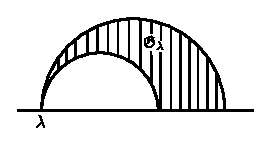
\includegraphics{figure1.eps}
\end{figure}

If $z\in\mathfrak{G}_{\lambda}$ and if $c_{1}\leq N(y_{A^{-1}})\leq
c_{2}$, then we claim that $z$ lies in a compact set in
$\mathfrak{H}_{n}$ depending on $c_{1}$, $c_{2}$ and on the choice of
$\epsilon_{1},\ldots,\epsilon_{n-1}$ and
$\alpha_{1},\ldots,\alpha_{n}$ in $K$. As a matter of fact, from
\eqref{150}, we know that
$$
\left|\log\left(\frac{y^{\ast}_{i}}{\sqrt[n]{N(y^{\ast})}}\right)\right|\leq
c_{3}\quad\text{for}\quad i=1,2,\ldots,n-1,
$$
and $|x^{\ast}_{j}|\leq c_{4}$ for $j=1,2,\ldots,n$. Hence we have
$$
c_{5}\leq \frac{y^{\ast}_{i}}{\sqrt[n]{N(y^{\ast})}}\leq
c_{6},\quad\text{for}\quad i=1,2,\ldots,n-1.
$$\pageoriginale
Since $c_{1}\leq N(y^{\ast})\leq c_{2}$, we have indeed for all
$i=1,2,\ldots,n$, 
$$
c_{7}\leq \frac{y^{\ast}_{i}}{\sqrt[n]{N(y^{\ast})}}\leq c_{8}.
$$
As a result, we obtain for $i$, $j=1,2,\ldots,n$,
\begin{align*}
c_{9} & \leq y^{\ast}_{i}\leq c_{10},\\
|x^{\ast}_{j}| & \leq c_{4},
\end{align*}
where $c_{9}$, $c_{10}$ and $c_{4}$ depend only on $c_{1}$, $c_{2}$
and the choice of $\epsilon_{1},\ldots,\epsilon_{n-1}$,
$\alpha_{1},\ldots,\alpha_{n}$ in $K$. Thus $z_{A^{-1}}$ and therefore
$z$ lies in a compact set in $\mathfrak{H}_{n}$, depending on $c_{1}$,
$c_{2}$ and $K$.

Now, we introduce the notion of {\em ``distance of a point
  $z\in\mathfrak{H}_{n}$ from a cusp $\lambda$ of
  $\mathfrak{H}_{n}$''}. We have already in $\mathfrak{H}_{n}$ a
metric given by
$$
ds^{2}=\sum^{n}_{i=1}\frac{dx^{2}_{i}+dy^{2}_{i}}{y^{2}_{i}}
$$
which is non-euclidean in the case $n=1$ and has an invariance
property with respect to $\Gamma$. But since the cusps lie on the
boundary of $\mathfrak{H}_{n}$, the distance (relative to this metric)
of an inner point of $\mathfrak{H}_{n}$ from a cusp is
infinite. Hence, this metric is not useful for our purposes.

For $z\in\mathfrak{H}_{n}$ and a cusp $\lambda=\rho/\sigma$ with
associated $A=\left(\begin{smallmatrix} \rho & \xi\\ \sigma & \eta
\end{smallmatrix}\right)\in \mathfrak{S}$, we define the {\em distance
  $\Delta(z,\lambda)$ of $z$ from $\lambda$} by
\begin{align*}
\Delta(z,\lambda)=(N(y_{A^{-1}}))^{-\frac{1}{2}} &= (N(y^{-1}|-\sigma
z+\rho|^{2}))^{\frac{1}{2}}\\
&= (N((-\sigma x+\rho)^{2}y^{-1}+\sigma^{2}y))^{\frac{1}{2}}.
\end{align*}
For $\lambda=\infty$, $\Delta(z,\infty)=1/\sqrt{N(y)}$; hence the
larger the $N(y)$, the `closer' is $z$ to $\infty$.

Now $\Delta(z,\lambda)$ has an important {\em invariance property}
with respect to $\Gamma$. Namely, for $M\in\Gamma$, we have
\begin{equation*}
\Delta(z_{M},\lambda_{M})=\Delta(z,\lambda).\tag{151}\label{151}
\end{equation*}
This\pageoriginale is very easy to verify, since, by definition
\begin{align*}
\Delta(z_{M},\lambda_{M}) &=
(N(\Iim(z_{M})_{A^{-1}M^{-1}}))^{-\frac{1}{2}}\\
&= (N(y_{A^{-1}}))^{-\frac{1}{2}}=\Delta(z,\lambda).
\end{align*}

Moreover, $\Delta(z,\lambda)$ does not depend on the special choice of
$A$ associated with $\lambda$. For, if
$A_{1}=\left(\begin{smallmatrix} \rho_{1} & \xi_{1}\\ \sim_{1} &
  \eta_{1}
\end{smallmatrix}\right)\in\mathfrak{S}$ is associated with
$\lambda=\rho_{1}/\sigma_{1}$, then
$A^{-1}A_{1}=T=\left(\begin{smallmatrix} \epsilon & \zeta\\ 0 &
  \epsilon^{-1}
\end{smallmatrix}\right)$ where $\epsilon$ is a unit in $K$. Now
$N(y_{A^{-1}_{1}})=N(y_{A^{-1}})N(\epsilon^{-2})=N(y_{A^{-1}})$ and
hence our assertion is proved.

Let, for a given cusp $\lambda$ and $r>0$, $\mathfrak{U}_{\lambda,r}$
denote the set of $z\in\mathfrak{H}_{n}$ such that
$\Delta(z,\lambda)<r$. This defines a `neighbourhood' of $\lambda$ and
all points $z\in\mathfrak{H}_{n}$ which belong to
$\mathfrak{U}_{\lambda,r}$ are inner points of the same. The
neighbourhoods, $\mathfrak{U}_{\lambda,r}$ for $0<r<\infty$ cover the
entire upper half-plane $\mathfrak{H}_{n}$. Each neighbourhood
$\mathfrak{U}_{\lambda,r}$ is left invariant by a modular substitution
in $\Gamma_{\lambda}$. For, by \eqref{151}, if $M\in\Gamma_{\lambda}$,
then
$$
\Delta (z_{M},\lambda)=\Delta(z_{M},\lambda_{M})=\Delta(z,\lambda)
$$
and so, if $z\in\mathfrak{U}_{\lambda,r}$, then again
$\Delta(z_{M},\lambda)<r$ \ie $z_{M}\in\mathfrak{U}_{\lambda,r}$. A
fundamental domain for $\Gamma_{\lambda}$ in
$\mathfrak{a}_{\lambda,r}$ is obviously given by
$\mathfrak{G}_{\lambda}\cap \mathfrak{U}_{\lambda,r}$.

We shall now prove some interesting facts concerning
$\Delta(z,\lambda)$ which will be useful in constructing a fundamental
domain for $\Gamma$ in $\mathfrak{H}_{n}$.
\begin{itemize}
\item[(i)] {\em For $z=x+iy\in \mathfrak{H}_{n}$, there exists a cusp
  $\lambda$ of $\mathfrak{H}_{n}$ such that for all cusps $\mu$ of
  $\mathfrak{H}_{n}$, we have}
\begin{equation*}
\Delta(z,\lambda)\leq \Delta(z,\mu).\tag{152}\label{152}
\end{equation*}
\end{itemize}

\begin{proof}
If $\lambda$ is a cusp, then $\lambda=\rho/\sigma$ for $\rho$,
$\sigma\in \mathfrak{o}$ such that $(\rho,\sigma)$ is one of the $h$
ideals $\mathfrak{U}_{1},\ldots,\mathfrak{U}_{h}$. Then
$$
\Delta(z,\lambda)=(N((-\sigma
x+\rho)^{2}y^{-1}+\sigma^{2}y))^{\frac{1}{2}}. 
$$
\end{proof}

Let us consider the expression $(N((-\sigma
x+\rho)^{2}y^{-1}+\sigma^{2}y))^{\frac{1}{2}}$ as a function of the
pair of integers $(\rho,\sigma)$. It remains unchanged if $\rho$,
$\sigma$ are replaced by $\rho\epsilon$, $\sigma\epsilon$ for any unit
$\epsilon$ in $K$. We shall now show that there exists a pair of
integers $\rho_{1}$, $\sigma_{1}$ in $K$ such that
\begin{equation*}
(N((-\sigma_{1}x+\rho_{1})^{2}y^{-1}+\sigma^{2}_{1}y))^{\frac{1}{2}}\leq
  (N((-\sigma x+\rho)^{2}y^{-1}+\sigma^{2}y))^{\frac{1}{2}}\tag{153}\label{153}
\end{equation*}\pageoriginale
for all pairs of integers $(\rho,\sigma)$. In order to prove
\eqref{153}, it obviously suffices to show that for given $C_{11}>0$,
there are only finitely many non-associated pairs of integers
$(\rho,\sigma)$ such that
\begin{equation*}
(N((-\sigma x+\rho)^{2}y^{-1}+\sigma^{2}y))^{\frac{1}{2}}\leq
  c_{11}.\tag{154}\label{154} 
\end{equation*}

Now, it is known from the theory of algebraic number fields that if
$\alpha=(\alpha_{1},\ldots,\alpha_{n})$ is an $n$-tuple of real
numbers with $N(\alpha)\neq 0$, then we can find a unit $\epsilon$ in
$K$ such that
\begin{equation*}
|\alpha_{i}\epsilon^{(i)}|\leq c_{12}|N(\alpha)|^{1/n}\tag{155}\label{155}
\end{equation*}
for a constant $c_{12}$ depending only on $K$. In view of \eqref{154},
we can suppose after multiplying $\rho$ and $\sigma$ by a suitable
unit $\epsilon$, that already we have
$$
(-\sigma^{(i)}x_{i}+\rho^{(i)})^{2}y_{i}^{-1}+\sigma^{(i)^{2}}_{y_{i}}\leq
c_{13},\quad i=1,2,\ldots,n,
$$
for a constant $c_{13}$ depending only on $c_{11}$ and $c_{12}$. This
implies that $(-\sigma^{(i)}x_{i}+\rho^{(i)})$ and $\sigma^{(i)}$ and
as a consequence $\rho^{(i)}$ and $\sigma^{(i)}$ are bounded, for
$i=1,2,\ldots,n$. Again, in this case, we know from the theory of
algebraic numbers that there are only finitely many possibilities for
$\rho$ and $\sigma$. Hence \eqref{154} is true only for finitely many
non-associated pairs of integers $(\rho,\sigma)$. From these pairs, we
choose a pair $(\rho_{1},\sigma_{1})$ such that the value of
$N((-\sigma_{1}x+\rho_{1})^{2}y^{-1}+\sigma^{2}_{1}y))^{\frac{1}{2}}$
is a minimum. This pair $(\rho_{1},\sigma_{1})$ now obviously
satisfies \eqref{153}.

Let $(\rho_{1},\sigma_{1})=\mathfrak{b}$ and let
$\mathfrak{b}=\mathfrak{a}_{i}(\theta)^{-1}$ for some
$\mathfrak{a}_{i}$ and a $\theta\in K$. Then
$\mathfrak{a}_{i}=(\rho_{1}\theta,\sigma_{1}\theta)$. Now, in
\eqref{153}, if we replace $\rho$, $\sigma$ by $\rho_{1}\theta$,
$\sigma_{1}\theta$ respectively, we get $|N(\theta)|\geq 1$. On the
other hand, since $\mathfrak{a}_{i}$ is of minimum norm among the
integral ideals of its class, $N(\mathfrak{a}_{i})\leq
N(\mathfrak{b})$ and therefore $|N(\theta)|\leq 1$. Thus
$|N(\theta)|=1$. Let now $\rho=\rho_{1}\theta$,
$\sigma=\sigma_{1}\theta$ and $\lambda=\rho/\sigma$. Then
$\mathfrak{a}_{i}=(\rho,\sigma)$ and by definition,
$\Delta(z,\lambda)=(N((-\sigma
x+\rho)^{2}y^{-1}+\sigma^{2}y))^{\frac{1}{2}}=(N((-\sigma_{1}x+\rho_{1})^{2}y^{-1}+\sigma^{2}_{1}y))^{\frac{1}{2}}$. If
we use \eqref{153}, then we see at once that $\Delta(z,\lambda)\leq
\Delta(z,\mu)$ for all cusps $\mu$.

For given $z\in \mathfrak{H}_{n}$, we define
$$
\Delta(z)=\inf_{\lambda}\Delta(z,\lambda).
$$
By\pageoriginale (i), there exists a cusp $\lambda$ such that
$\Delta(z,\lambda)=\Delta(z)$. In general, $\lambda$ is unique, but
there are exceptional cases when the minimum is attained for more than
one $\lambda$. We shall see presently that there exists a constant
$d>0$, depending only on $K$ such that if $\Delta(z)<d$, then the cusp
$\lambda$ for which $\Delta(z,\lambda)=\Delta(z)$ is unique.
\begin{itemize}
\item[(ii)] {\em There exists $d>0$ depending only on $K$, such that,
  if for $z=x+iy\in\mathfrak{H}_{n}$, $\Delta(z,\lambda)<d$ and
  $\Delta(z,\mu)<d$, then necessarily $\lambda=\mu$.} 
\end{itemize}

\begin{proof}
Let $\lambda=\rho/\sigma$ and $\mu=\rho_{1}/\sigma_{1}$ and let for a
real number $d>0$,
\begin{align*}
\Delta(z,\lambda) &= (N((-\sigma
x+\rho)^{2}y^{-1}+\sigma^{2}y))^{\frac{1}{2}}<d,\\
\Delta(z,\mu) &=
(N(-\sigma_{1}x+\rho_{1})^{2}y^{-1}+\sigma^{2}_{1}y)^{\frac{1}{2}}<d. 
\end{align*}
After multiplying $\rho$ and $\sigma$ by a suitable unit $\epsilon$ in
$K$, we might assume in view of \eqref{155} that
$$
(\sigma^{(i)}x_{i}-\rho^{(i)})^{2}y^{-1}_{i}+\sigma^{(i)^{2}}y_{i}<c_{12}d^{2/n},\quad
i=1,2,\ldots,n. 
$$
Hence
\begin{align*}
|-\sigma^{(i)}x_{i}+\rho^{(i)}|y^{-\frac{1}{2}}_{i} &<
\sqrt{c_{12}}d^{1/n},\\
|\sigma^{(i)}|y^{\frac{1}{2}}_{i} &< \sqrt{c_{12}}d^{1/n}. 
\end{align*}
Similarly we have
\begin{align*}
|-\sigma^{(i)}_{1}x_{i}+\rho^{(i)}_{1}|y^{-\frac{1}{2}}_{i} &<
\sqrt{c_{12}}d^{1/n},\\
|\sigma^{(i)}_{1}|y^{\frac{1}{2}}_{i} &< \sqrt{c_{12}}d^{1/n}.
\end{align*}
Now
$$
\rho^{(i)}\sigma^{(i)}_{1}-\rho^{(i)}_{1}\sigma^{(i)}=(-\sigma^{(i)}x_{i}+\rho^{(i)})y^{-\frac{1}{2}}_{i}\sigma^{(i)}_{1}y^{\frac{1}{2}}_{i}-(-\sigma^{(i)}_{1}x_{i}+\rho^{(i)}_{1})y^{-\frac{1}{2}}_{i}\sigma^{(i)}y^{\frac{1}{2}}_{i}
$$
and hence
$$
|N(\rho\sigma_{1}-\sigma\rho_{1})|<(2c_{12}d^{2/n})^{n}.
$$
If\pageoriginale we set $d=(2c_{12})^{-n/2}$, then
$|N(\rho\sigma_{1}-\sigma\rho_{1})|<1$. Since
$\rho\sigma_{1}-\sigma\rho_{1}$ is an integer, it follows that
$\rho\sigma_{1}-\sigma\rho_{1}=0$ \ie $\lambda=\mu$.
\end{proof}

Thus for $d=(2c_{12})^{-n/2}$, the conditions $\Delta(z,\lambda)<d$,
$\Delta(z,\mu)<d$ for a $z\in\mathfrak{H}_{n}$ imply that
$\lambda=\mu$. Therefore, the neighbourhoods
$\mathfrak{U}_{\lambda,d}$ for the various cusps $\lambda$ are
mutually disjoint.

We shall now prove that for $z\in\mathfrak{H}_{n}$, $\Delta(z)$ is
uniformly bounded in $\mathfrak{H}_{n}$. To this end, it suffices to
prove

\begin{itemize}
\item[(iii)] {\em There exists $c>0$ depending only on $K$ such that
  for any $z=x+iy\in\mathfrak{H}_{n}$, there exists a cusp $\lambda$
  with the property that $\Delta(z,\lambda)<c$.}
\end{itemize}

\begin{proof}
We shall prove the existence of a constant $c>0$ depending only on $K$
and a pair of integers $(\rho,\sigma)$ not both zero such that
$$
(N((-\sigma x+\rho)^{2}y^{-1}+\sigma^{2}y))^{\frac{1}{2}}<c.
$$

Let $\omega_{1},\ldots,\omega_{n}$ be a basis of
$\mathfrak{o}$. Consider now the following system of $2n$ linear
inequalities in the $2n$ variables $a_{1},\ldots,a_{n}$,
$b_{1},\ldots,b_{n}$, viz.
$$
\left|y^{-\frac{1}{2}}_{k}(\omega^{(k)}_{1}a_{1}+\cdots+\omega^{(k)}_{n}a_{n})-x_{k}y^{-\frac{1}{2}}_{k}(\omega^{(k)}_{1}b_{1}+\cdots+\omega^{(k)}_{n}b_{n})\right|\leq
\alpha_{k} 
$$
for $k=1,2,\ldots,n$ and
$$
\left|y^{\frac{1}{2}}_{k}(\omega^{(k)}_{1}b_{1}+\cdots+\omega^{(k)}_{n}b_{n})\right|\leq
\beta_{k} 
$$
for $k=1,\ldots,n$.
\end{proof}

The determinant of this system of linear forms is
$|(\omega^{(j)}_{i})|^{2}=|\Delta|$ where $\Delta$ is the discriminant
of $K$. By Minkowski's theorem on linear forms, this system of linear
inequalities has a nontrivial solution in rational integers
$a_{1},\ldots,a_{n}$, $b_{1},\ldots,b_{n}$ if
$\alpha_{1},\ldots,\alpha_{n}\cdot \beta_{1},\ldots,\beta_{n}\leq
|\Delta|$. Taking
$\alpha_{i}=\beta_{j}=\sqrt[2n]{|\Delta|}i=1,2,\ldots,n,j=1,2,\ldots,n$,
in particular, this system of inequalities has a nontrivial solution
in rational integers, say, $a'_{1},\ldots,a'_{n}$,
$b'_{1},\ldots,b'_{n}$. Let us take
$\rho=a'_{1}\omega_{1}+\cdots+a'_{n}\omega_{n}$ and
$\sigma=b'_{1}\omega_{1}+\cdots+b'_{n}\omega_{n}$. Then we obtain
$$
\left|(-\sigma^{(i)}x_{i}+\rho^{(i)})^{2}y^{-1}_{i}+\sigma^{(i)^{2}}y_{i}\right|\leq
\sqrt[2n]{|\Delta|},\quad i=1,2,\ldots,n. 
$$
Hence\pageoriginale $(N((-\sigma
x+\rho)^{2}y^{-1}+\sigma^{2}y))^{\frac{1}{2}}\leq
2^{n/2}|\Delta|^{\frac{1}{2}}=c$ (say). 

Now let $(\rho,\sigma)=\mathfrak{b}$;
$\mathfrak{b}=\mathfrak{a}_{i}(\theta)^{-1}$ for some
$\mathfrak{a}_{i}$ and for some $\theta\in K$. Since
$\mathfrak{a}_{i}$ is of minimum norm among the integral ideals of its
class, $|N(\theta)|\leq 1$. Further
$\mathfrak{a}_{i}=(\rho\theta,\sigma\theta)$. Now, for the cusp
$\lambda=\rho\theta/\sigma\theta=\rho/\sigma$, we have
$$
\Delta(z,\lambda)=|N(\theta)|(N((-\sigma
x+\rho)^{2}y^{-1}+\sigma^{2}y))^{\frac{1}{2}}\leq c,
$$
which was what we wished to prove.

From (iii), we deduce that
$\mathfrak{H}_{n}=\bigcup\limits_{\lambda}\mathfrak{U}_{\lambda,c}$.

\begin{itemize}
\item[(iv)] {\em For $z\in\mathfrak{H}_{n}$ and $M\in\Gamma$,
  $\Delta(z_{M})=\Delta(z)$.} 
\end{itemize}

\begin{proof}
In fact,
\begin{align*}
\Delta(z_{M}) &= \inf\limits_{\lambda}\Delta(z_{M},\lambda)\\
&= \inf\limits_{\lambda}\Delta(z,\lambda_{M^{-1}}) \quad \text{(by \eqref{151})}\\
&= \inf\limits_{\lambda}\Delta(z,\lambda)\\
&=\Delta(z).
\end{align*}
\end{proof}

We now have all the necessary material for the construction of a
fundamental domain for $\Gamma$ in $\mathfrak{H}_{n}$.

A point $z\in\mathfrak{H}_{n}$ is {\em semi-reduced} ({\em with
  respect to a} cups $\lambda$), if $\Delta(z)=\Delta(z,\lambda)$. If
$z$ is semi-reduced with respect to $\lambda$, then for all cusps
$\mu$, we have $\Delta(z,\mu)\geq \Delta(z,\lambda)$.

Let $\lambda_{1}(=(\infty,\ldots,\infty))$,
$\lambda_{2},\ldots,\lambda_{h}$ be the $h$ inequivalent base cusps of
$\mathfrak{H}_{n}$. We denote by $\mathfrak{F}_{\lambda_{i}}$, the set
of all $z\in\mathfrak{H}_{n}$ which are semi-reduced with respect to
$\lambda_{i}$. Clearly $\mathfrak{F}_{\lambda_{i}}\subset
\mathfrak{U}i_{\lambda_{i,c}}$, in view of (iii) above. The set
$\mathfrak{F}_{\lambda_{i}}$ is invariant under the modular
substitution $z\to z_{M}$, for $M\in\Gamma_{\lambda_{i}}$. For, by
(iv) above, $\Delta(z_{M})=\Delta(z)$ and further.
$$
\Delta(z)=\Delta(z,\lambda_{i})=\Delta(z_{M},(\lambda_{i})_{M})=\Delta(z_{M},\lambda_{i}). 
$$
Thus $\Delta(z_{M})=\Delta(z_{M},\lambda_{i})$ and hence $z_{M}\in
\mathfrak{F}_{\lambda_{i}}$, for $M\in\Gamma_{\lambda_{i}}$. 

Let $\ob{\mathfrak{G}}_{\lambda_{i}}$ denote the closure in
$\mathfrak{H}_{n}$ of the set $\mathfrak{G}_{\lambda_{i}}$ and
$\mathfrak{q}_{i}=\mathfrak{F}_{\lambda_{i}}\cap
\ob{\mathfrak{G}}_{\lambda_{i}}$. Then $\mathfrak{q}_{i}$ is
explicitly defined as the set of $z\in\mathfrak{H}_{n}$ whose local
coordinates $X_{1},\ldots,X_{n}$,\pageoriginale $Y_{1},\ldots,Y_{n-1}$
relative to the cusp $\lambda_{i}$ satisfy the conditions
$$
-\frac{1}{2}\leq X_{k}\leq \frac{1}{2},-\frac{1}{2}\leq Y_{l}\leq
\frac{1}{2}(k=1,2,\ldots,n;l=1,2,\ldots,n-1) 
$$
and further, for all cusps $\mu$,
$$
\Delta(z,\mu)\geq \Delta(z,\lambda_{i}).
$$
Let $\mathfrak{F}=\cup^{h}_{i=1}\mathfrak{q}_{i}$. We see that the
$\mathfrak{q}_{i}$ as also $\mathfrak{F}$ are closed in
$\mathfrak{H}_{n}$.

A point $z\in\mathfrak{q}_{i}$ is an {\em inner point} of
$\mathfrak{q}_{i}$ if in all the conditions above, strict inequality
holds, viz.
\begin{align*}
-\frac{1}{2}<X_{k}<\frac{1}{2},-\frac{1}{2}<Y_{l} &<
\frac{1}{2}(k=1,2,\ldots,n,l=1,2,\ldots,n-1)\\
\Delta(z,\mu) &> \Delta(z,\lambda_{i}),\text{ \ for \ } \mu\neq
\lambda_{i}.\tag{$150^{\ast}$}\label{150*} 
\end{align*}
If equality holds even in one of these conditions, then $z$ is said to
be a {\em boundary point} of $\mathfrak{q}_{i}$. The set of boundary
points of $\mathfrak{q}_{i}$ constitute the boundary of
$\mathfrak{q}_{i}$, which may be denoted by $Bd$
$\mathfrak{q}_{i}$. We denote by $\mathfrak{R}_{i}$, the set of inner
points of $\mathfrak{q}_{i}$.

It is clear that the $\mathfrak{q}_{i}$ do not overlap and intersect
at most on their boundary.

A point $z\in\mathfrak{F}$ may now be called an {\em inner point} of
$\mathfrak{F}$, if $z$ is an inner point of some $\mathfrak{q}_{i}$;
similarly we may define a {\em boundary point} of $\mathfrak{F}$ and
denote the set of boundary points of $\mathfrak{F}$ by $Bd$
$\mathfrak{F}$.

We say that a point $z\in\mathfrak{H}_{n}$ is {\em reduced} (with
respect to $\Gamma$) if, in the first place, $z$ is semi-reduced with
respect to some one of the $h$ cusps $\lambda_{1},\ldots,\lambda_{h}$,
say $\lambda_{i}$ and then further
$z\in\ob{\mathfrak{G}}_{\lambda_{i}}$. Clearly $\mathfrak{F}$ {\em is just
the set of all $z\in\mathfrak{H}_{n}$ reduced with respect to
$\Gamma$.}

Before we proceed to show that $\mathfrak{F}$ is a fundamental domain
for $\Gamma$ in $\mathfrak{H}_{n}$, we shall prove the following
result concerning the inner points of $\mathfrak{F}$, namely,

{\em The set of inner points of $\mathfrak{F}$ is open in
  $\mathfrak{H}_{n}$.}

\begin{proof}
It is enough to show that each $\mathfrak{R}_{j}$ is open in
$\mathfrak{H}_{n}$. Let, then, $z_{0}=x_{0}+iy_{0}\in
\mathfrak{R}_{j}$; we have to prove that there exists a neighbourhood
$V$ of $z_{0}$ in $\mathfrak{H}_{n}$ which is wholly contained in
$\mathfrak{R}_{j}$. 
\end{proof}

Now,\pageoriginale for each $z=x+iy\in\mathfrak{H}_{n}$ and a cusp
$\mu=\rho/\sigma$, we have $\Delta(z,\mu)=(N((-\sigma
x+\rho)^{2}y^{-1}+\sigma^{2}y))^{\frac{1}{2}}$. Using the fact that
for each $j=1,2,\ldots,n$,
$(-\sigma^{(j)}x_{j}+\rho^{(j)})^{2}y^{-1}+\sigma^{(j)^{2}}y_{j}$ is a
positive-definite binary quadratic form in $\sigma^{(j)}$ and
$\rho^{(j)}$, we can easily show that
$$
\Delta(z,\mu)\geq \alpha(N(\sigma^{2}+\rho^{2}))^{\frac{1}{2}}
$$
where $\alpha=\alpha(z)$ depends continuously on $z$ and does not
depend on $\mu$. We can now find a sufficiently small neighbourhood
$W$ of $z_{0}$ such that for all $z\in W$,
$$
\Delta(z,\mu)\geq
\frac{1}{2}\alpha_{0}(N(\sigma^{2}+\rho^{2}))^{\frac{1}{2}}
$$
where $\alpha_{0}=\alpha(z_{0})$. Moreover, we can assume $W$ so
chosen that for all $z\in W$,
$$
\Delta(z,\lambda_{j})\leq 2\Delta(z_{0},\lambda_{j}).
$$
Thus, for all cusps $\mu=\rho/\sigma$ and $z\in W$,
$$
\Delta(z,\mu)-\Delta(z,\lambda_{j})\geq
\frac{1}{2}\alpha_{0}(N(\sigma^{2}+\rho^{2}))^{\frac{1}{2}}-2\Delta(z_{0},\lambda_{j}).
$$

Now, employing an argument used already on p.\@ 198, we can show that
there are only finitely many non-associated pairs of integers
$(\rho,\sigma)$ such that
$$
\frac{1}{2}\alpha_{0}(N(\sigma^{2}+\rho^{2}))^{\frac{1}{2}}\leq
2\Delta(z_{0},\lambda_{j}). 
$$
It is an immediate consequence that except for finitely many cusps
$\mu_{1},\break\ldots,\mu_{r}$, we have for $\mu\neq \lambda_{j}$,
$$
\Delta(z,\mu)>\Delta(z,\lambda_{j}).
$$
Now, since $\Delta(z_{0},\mu)>\Delta(z_{0},\lambda_{j})$ for all cusps
$\mu\neq \lambda_{j}$, we can, in view of the continuity in $z$ of
$\Delta(z,\mu_{i})$ (for $i=1,2,\ldots,r$) find a neighbourhood $U$ of
$z_{0}$ such that
$$
\Delta(z,\mu_{k})>\Delta(z,\lambda_{j})\quad (k=1,2,\ldots,r)
$$
for\pageoriginale $z\in U$ and $\mu_{k}\neq \lambda_{j}$. We then have
finally for all $z\in U\cap W$
$$
\Delta(z,\mu)>\Delta(z,\lambda_{j})
$$
provided $\mu\neq \lambda_{j}$. Further, we could have chosen $U$ such
that for all $z\in U$, \eqref{150*} is satisfied, in addition. Thus
the neighbourhood $V=U\cap W$ of $z_{0}$ satisfies our requirements
and so $\mathfrak{R}_{j}$ is open.

It may now be seen that the closure $\ob{\mathfrak{R}}_{i}$ of
$\mathfrak{R}_{i}$ is just $\mathfrak{q}_{i}$. In fact, let $z\in
\mathfrak{q}_{i}$ and let $\lambda_{i}=\infty_{A_{i}}$,
$z^{\ast}=z_{A^{-1}_{i}}$, $\mu_{A^{-1}_{i}}=\nu=\rho/\sigma\neq
\infty$. Then we have
$$
\sigma\neq 0,
\frac{\Delta(z,\mu)}{\Delta(z,\lambda_{i})}=\frac{\Delta(z^{\ast},\nu)}{\Delta(z^{\ast},\infty)}=(N((-\sigma
x^{\ast}+\rho)^{2}+(\sigma y^{\ast})^{2}))^{\frac{1}{2}}.
$$
If $y^{\ast}$ is replaces by $ty^{\ast}$ where $t$ is a positive
scalar factor, then the expression above is a strictly monotonic
increasing function of $t$, whereas the coordinates
$X_{1},\ldots,X_{n}$, $Y_{1},\ldots,Y_{n-1}$ remain unchanged. Thus,
if $z\in\mathfrak{q}_{i}$ and
$z_{A^{-1}_{i}}=z^{\ast}=x^{\ast}+iy^{\ast}$, then for
$z^{(t)}=(x^{\ast}+ity^{\ast})_{A_{i}}$, $t>1$, the inequalities
$\Delta(z,\mu)>\Delta(z,\lambda_{i})(\mu\neq \lambda_{i})$ are
satisfied and moreover for a small change in the coordinates
$X_{1},\ldots,X_{n}$, $Y_{1},\ldots,Y_{n-1}$, the inequalities
\eqref{150*} are also satisfied. As a consequence, if
$z\in\mathfrak{q}_{i}$, then every neighbourhood of $z$ intersects
$\mathfrak{R}_{i}$; in other words,
$\ob{\mathfrak{R}}_{i}=\mathfrak{q}_{i}$.

From above, we have that if $z\in \mathfrak{q}_{i}$, then the entire
curve defined by $z^{(t)}=(x^{\ast}+ity^{\ast})_{A_{i}}$, $t\geq 1$
lies in $\mathfrak{q}_{i}$ and hence for $z\in\mathfrak{R}_{i}$, in
particular, $z^{(t)}$ for large $t>0$ belongs to $\mathfrak{R}_{i}$,
Using this it may be shown that $\mathfrak{q}_{i}$ and similarly
$\mathfrak{R}_{i}$ are connected.

The existence of inner points of $\mathfrak{q}_{j}$ is an immediate
consequence of result (ii) on p.\@ 199. For $j=1$, it may be verified
that $z=(it,\ldots,it)$, $t>1$ is an inner point of
$\mathfrak{q}_{1}$.

Now we proceed to prove that $\mathfrak{F}$ is a fundamental domain
for $\Gamma$ in $\mathfrak{H}_{n}$. We have first to show that
\begin{itemize}
\item[$(\alpha)$] {\em the images $\mathfrak{F}_{M}$ of $\mathfrak{F}$
  for $M\in\Gamma$ cover $\mathfrak{H}_{n}$ without gaps.}
\end{itemize}

\begin{proof}
This is obvious from the very method of construction of
$\mathfrak{F}$. First, for any $z\in\mathfrak{H}_{n}$, there exists a
cusp $\lambda$ such that $\Delta(z)=\Delta(z,\lambda)$. Let
$\lambda=(\lambda_{i})_{M}$ for some $\lambda_{i}$ and
$M\in\Gamma$. We have then
$$
\Delta(z_{M^{-1}})=\Delta(z)=\Delta(z,\lambda)=\Delta(z_{M^{-1}},\lambda_{i})
$$\pageoriginale
and hence $z_{M^{-1}}\in\mathfrak{F}_{\lambda_{i}}$. Now we can find
$N\in\Gamma_{\lambda_{i}}$ such that $(z_{M^{-1}})_{N}$ is reduced
with respect to $\Gamma_{\lambda_{i}}$ and thus
$z_{NM^{-1}}\in\mathfrak{F}$.
\end{proof}

Next, we show that
\begin{itemize}
\item[$(\beta)$] {\em the images $\mathfrak{F}_{M}$ of $\mathfrak{F}$
  for $M\in\Gamma$ cover $\mathfrak{H}_{n}$ without overlaps.}
\end{itemize}

\begin{proof}
Let $z_{1}$, $z_{2}\in\mathfrak{F}$ such that $z_{1}=(z_{2})_{M}$ for
an $M\neq \pm\left(\begin{smallmatrix} 1 & 0\\ 0 & 1
\end{smallmatrix}\right)$ in $\Gamma$ and let
$z_{1}\in\mathfrak{q}_{i}$ and $z_{2}\in\mathfrak{q}_{j}$. Now, since
$z_{1}\in\mathfrak{F}_{\lambda_{i}}$, we have
$$
\Delta(z_{1},\lambda_{i})\leq
\Delta(z_{1},(\lambda_{j})_{M})=\Delta(z_{2},\lambda_{j}).
$$
Similarly
$$
\Delta(z_{2},\lambda_{j})\leq
\Delta(z_{2},(\lambda_{i})_{M^{-1}})=\Delta(z_{1},\lambda_{i}).
$$
Therefore, we obtain
$$
\Delta(z_{1},\lambda_{i})=\Delta(z_{2},\lambda_{j})=\Delta(z_{1},(\lambda_{j})_{M}).
$$
\end{proof}

Let us first suppose that
$\Delta(z_{1},\lambda_{i})=\Delta(z_{2},\lambda_{j})<d$. Then, since
$\Delta(z_{1},\lambda_{i})<d$ as also
$\Delta(z_{1},(\lambda_{j})_{M})<d$, we infer from the result (ii) on
p.\@ 199 that $\lambda_{i}=(\lambda_{j})_{M}$. But $\lambda_{i}$ and
$\lambda_{j}$, for $i\neq j$ are not equivalent with respect to
$\Gamma$. Therefore $i=j$ and $M\in\Gamma_{\lambda_{i}}$. Again, since
both $z_{1}$ and $z_{2}$ are in $\ob{\mathfrak{G}}_{\lambda_{i}}$ and
further $z_{1}=(z_{2})_{M}$ with $M\in\Gamma_{\lambda_{i}}$, we
conclude that necessarily $z_{1}$ and $z_{2}$ belong to
$Bd\mathfrak{F}$ and indeed their local coordinates
$X_{1},\ldots,X_{n}$, $Y_{1},\ldots,Y_{n-1}$ relative to $\lambda_{i}$
satisfy at least one of the finite number of conditions $X_{1}=\pm
1/2,\ldots,X_{n}=\pm 1/2$, $Y_{1}=\pm 1/2,\ldots,Y_{n-1}=\pm
1/2$. Further $M$ clearly belongs to a finite set $M_{1},\ldots,M_{r}$
of elements in $\bigcup\limits^{h}_{i=1}\Gamma_{\lambda_{i}}$.

We have now to deal with the case
$$
d\leq \Delta(z_{1},\lambda_{i})\leq c\text{ \ and \ } d\leq
\Delta(z_{2},\lambda_{j})\leq c
$$
where we may suppose that $\lambda_{i}\neq (\lambda_{j})_{M}$. Let,
for $i=1,2,\ldots,h$, $B_{i}$ denote the set of $z\in\mathfrak{H}_{n}$
for which $d\leq \Delta(z,\lambda_{i})\leq c$ and
$z\in\ob{\mathfrak{G}}_{\lambda_{i}}$. Then, by our remark on p.\@ 196
$B_{i}$ is compact and so is
$B=\bigcup\limits^{\hat{h}}_{i=1}B_{i}$. Now, both $z_{2}$ and
$z_{1}=(z_{2})_{M}$ belong to the compact set $B$. We may then deduce
from Proposition \ref{prop21} that $M$ belongs to a finite set of
elements $M_{r+1},\ldots,M_{s}$\pageoriginale in $\Gamma$, depending
only on $B$ and hence only on $K$. Moreover $z_{1}$ satisfies
$$
\Delta(z_{1},\lambda_{i})=\Delta(z_{1},(\lambda_{j})_{M})
$$
with $(\lambda_{j})_{M}\neq\lambda_{i}$. Hence $z_{1}$ and similarly
$z_{2}$ belongs to $Bd\mathfrak{F}$. As a result, arbitrarily near
$z_{1}$ and $z_{2}$, there exist points $z$ such that
$\Delta(z,\lambda_{i})\neq \Delta(z,(\lambda_{j})_{M})$ for
$M=M_{r+1},\ldots,M_{s}$. 

Thus, finally, no two inner points of $\mathfrak{F}$ can be equivalent
with respect to $\Gamma$. Further $\mathfrak{F}$ intersects only
finitely many of its neighbours
$\mathfrak{F}_{M_{1}},\ldots,\mathfrak{F}_{M_{s}}$ and indeed only on
its boundary. We have therefore established (ii).

From $(\alpha)$ and $(\beta)$ above, it follows that $\mathfrak{F}$ is
a fundamental domain for $\Gamma$ in $\mathfrak{H}_{n}$. It consists
of $h$ connected `pieces' corresponding to the $h$ inequivalent base
cusps $\lambda_{1},\ldots,\lambda_{h}$ and is bounded by a finite
number of `manifolds' of the form
\begin{equation*}
\Delta(z,\lambda_{i})=\Delta(z,(\lambda_{j})_{M}),i,j=1,2,\ldots,h,M=M_{r+1},\ldots,M_{s}\tag{156}\label{156} 
\end{equation*}
and the hypersurfaces defined by
$$
X^{(k)}_{i}=\pm \frac{1}{2}, Y^{(k)}_{j}=\pm
\frac{1}{2},i=1,2,\ldots,n; j=1,2,\ldots,n-1
$$
where $X^{(k)}_{1},\ldots,X^{(k)}_{n}$,
$Y^{(k)}_{1},\ldots,Y^{(k)}_{n-1}$ are local coordinates relative to
the base cusp $\lambda_{k}$.

The `manifolds' defined by \eqref{156} are seen to be generalizations
of the `isometric circles', in the sense of Ford, for a fuchsian
group. In fact, if $\lambda_{i}=\rho_{i}/\sigma_{i}$ and
$(\lambda_{j})_{M}=\rho/\sigma$, then the condition \eqref{156} is
just
$$
N(|-\sigma_{i}z+\rho_{i}|)=N(|-\sigma z+\rho|).
$$
If we set $n=1$ and $\lambda_{i}=\infty$ or equivalently $\rho_{i}=1$
and $\sigma_{i}=0$, then the condition reads as
$$
|-\sigma z+\rho|=1
$$
which is the familiar `isometric circle' corresponding to the
transformation $z\to \dfrac{\eta z-\xi}{-\sigma z+\rho}$ of
$\mathfrak{H}_{1}$ onto itself.

The conditions $\Delta(z,\lambda)\geq \Delta(z,\lambda_{i})$ by which
$\mathfrak{F}_{\lambda_{i}}$ was defined, simply mean for $n=1$ and
$\lambda_{i}=\infty$ that $|\gamma z+\delta|\geq 1$ for all pairs of
coprime rational\pageoriginale integers $(\gamma,\delta)$. Thus, just
as the points of the well-known fundamental domain in
$\mathfrak{H}_{1}$ for the elliptic modular group lie in the exterior
of the the isometric circles $|\gamma z+\delta|=1$ corresponding to
the same group, $\mathfrak{F}_{\lambda_{i}}$ lies in the `exterior' of
the generalized isometric circles
$\Delta(z,\lambda_{i})=\Delta(z,\lambda)$.

We now prove the following important result, which will be used later.

\begin{proposition}\label{prop22}
Let $\mathfrak{F}^{\ast}$ denote the set of $z\in\mathfrak{F}$ for
which $\Delta(z,\lambda_{i})\geq e_{i}>0$, $i=1,2,\ldots,h$. Then
$\mathfrak{F}^{\ast}$ is compact in $\mathfrak{H}_{n}$.
\end{proposition}

The {\em proof} is almost trivial in the light of our remark on p.\@
196. Let $B_{i}$ denote the set of $z\in\mathfrak{G}_{\lambda_{i}}$
for which $e_{i}\leq \Delta(z,\lambda_{i})\leq c$. Then $B_{i}$ as
also $B=\cup^{h}_{i=1}B_{i}$ is compact in $\mathfrak{H}_{n}$. Hence
$\mathfrak{F}^{\ast}$ which is closed and contained in $B$, is again
compact.

Suppose instead of $\mathfrak{H}_{n}$, we consider the space
$\mathfrak{H}^{\ast}_{n}$ of $(z_{1},\ldots,z_{n})\in C^{n}$ with
$\Iim(z_{1})<0$ and $\Iim(z_{i})>0$ for $i=2,\ldots,n$. Then by means
of the mapping $(z_{1},\ldots,z_{n})\to
(\ob{z}_{1},z_{2},\ldots,z_{n})$ of $\mathfrak{h}_{n}$ onto
$\mathfrak{H}^{\ast}_{n}$, $\mathfrak{F}$ goes over into a fundamental
domain for $\Gamma$ in $\mathfrak{H}^{\ast}_{n}$. The general case
when we take instead of $\mathfrak{H}_{n}$, the product of $r$ upper
half-planes and $n-r$ lower half-planes, can be dealt with, in a
similar fashion.

It was Blumenthal who first gave a method of constructing a
fundamental domain for $\Gamma$ in $\mathfrak{H}_{n}$ but his proof
contained an error since he obtained a fundamental domain with just
one cusp and not $h$ cusps. This error was set right by Maass.

We remark finally that our method of constructing the fundamental
domain $\mathfrak{F}$ is essentially different from the well-known
method of Fricke for constructing a `normal polygon' for a
discontinuous group of analytic automorphisms of a bounded domain in
the complex plane. Our method uses only the notion of ``distance of a
point of $\mathfrak{H}_{n}$ from a cusp'', whereas we require a metric
invariant under the group, for Fricke's method which is as
follows. Let $G$ be a bounded domain in the complex plane and
$\Gamma$, a discontinuous group of analytic automorphisms of
$G$. Further let $G$ possess a metric $D(z_{1},z_{2})$ for $z_{1}$,
$z_{2}\in G$, having the property that
$D((z_{1})_{M},(z_{2})_{M})=D(z_{1},z_{2})$ for $M\in \Gamma$. We
choose a point $z_{0}$ which is not a fixed point of any $M\in\Gamma$,
other than the identity and a fundamental domain for $\Gamma$ in $G$
is given by the set of points $z\in G$ for which 
$$
D(z,(z_{0})_{M})\geq D(z,z_{0})\text{ \ for all \ } M\in \Gamma.
$$\pageoriginale

Now we know that $\mathfrak{H}_{n}$ carries a Riemannian metric which
is invariant under $\Gamma$. Suppose we use this metric and try to
adapt Fricke's method of constructing a fundamental domain. For our
later purposes, we require a fundamental domain whose nature near the
cusps should be well known. Therefore we see in the first place that
the adaptation of Fricke's method to our case is not practical in view
of the fact that the distance of a point of $\mathfrak{H}_{n}$ from
the cusps, relative to the Riemannian metric, is infinite. In the
second place, it is advantageous to adapt Fricke's method only when
the fundamental domain is compact, whereas we know that the
fundamental domain is not compact in our case. Moreover, our method of
construction of the fundamental domain uses the deep and intrinsic
properties of algebraic number fields.

The following proposition is necessary for our later purposes.

\begin{proposition}\label{prop23}
For any compact set $C$ in $\mathfrak{H}_{n}$, there exists a constant
$b=b(C)>0$ such that $C\cap \mathfrak{U}_{\mu,b}\neq \emptyset$ for
all cusps $\mu$.
\end{proposition}

\begin{proof}
Since $C$ is compact, we can find $\alpha$, $\beta>0$ depending only
on $C$ such that for $z=x+iy\in C$, we have $\beta\leq N(y)\leq
\alpha$. Now, for any cusp
$\lambda=(\rho/\sigma)(\rho,\sigma\in\mathfrak{o})$ and $z=x+iy\in C$,
it is clear that $\Delta(z,\lambda)=(N((-\sigma
x+\rho)^{2}y^{-1}+\sigma^{2}y))^{1/2}$ satisfies
$$
\Delta(z,\lambda)\geq
\begin{cases}
|N(\sigma)|N(y)^{\frac{1}{2}}\geq \beta^{\frac{1}{2}},\text{ \ for \ }
\sigma\neq 0\\
|N(\rho)|N(y)^{-\frac{1}{2}}\geq \alpha^{-\frac{1}{2}}, \text{ \ for
  \ } \sigma=0.
\end{cases}
$$
If we choose $b$ for which
$0<b<\min(\alpha^{-\frac{1}{2}},\beta^{\frac{1}{2}})$, then it is
obvious that for {\em all} cusps $\lambda$,
$\mathfrak{U}_{\lambda,b}\cap C=\emptyset$.
\end{proof}

\section{Hilbert modular functions}\label{chap3:sec3}

We shall first develop here some properties of (entire) Hilbert
modular forms and, in particular, show that a Hilbert modular form
satisfies the regularity condition at the cusps of the fundamental
domain $\mathfrak{F}$, automatically for $n\geq 2$. We shall then
prove the existence of $n+1$ (entire) modular\pageoriginale forms
$f_{0}(z),f_{1}(z),\ldots,f_{n}(z)$ of `large' weight $k$ such that
the functions
$\dfrac{f_{1}(z)}{f_{0}(z)},\ldots,\dfrac{f_{n}(z)}{f_{0}(z)}$ are
analytically independent. Next, we shall obtain estimates for the
dimensions of the space of entire modular forms of `large'
weight. Finally, we shall show that every Hilbert modular function can
be expressed as the quotient of two Hilbert modular forms of the same
weight and use this result to prove the {\em main theorem} that the
Hilbert modular functions form an algebraic function field of $n$
variables over the field of complex numbers.

Let $K$ be a totally real algebraic number field of degree $n$ over
$R$ and let $\Gamma$ be the corresponding Hilbert modular
group. Further let $k$ be a rational integer.

A complex-valued function $f(z)$ defined in $\mathfrak{H}_{n}$ is
called an {\em entire Hilbert modular form of weight $k$} (or {\em of
  dimension-$k$}) {\em belonging to the group $\Gamma$,} if
\begin{itemize}
\item[(1)] $f(z)$ is regular in $\mathfrak{H}_{n}$,

\item[(2)] for every
\begin{equation*}
M=\left(\begin{smallmatrix} 
\alpha &  \beta\\
 \gamma & \delta
\end{smallmatrix}\right)\in\Gamma,
  f(z_{M})N(\gamma z+\delta)^{-k}=f(z), \tag{157}\label{157}
\end{equation*}

\item[(3)] for every cusp $\lambda_{i}=\rho_{i}/\sigma_{i}$ of
  $\mathfrak{F}$, $f(z)N(-\sigma_{i}z+\rho_{i})^{k}$ is regular at the
  cusp $\lambda_{i}$ \ie it has a Fourier expansion of the form
  $c(0)+\sum\limits_{\beta}c(\beta)e^{2\pi iS(\beta z_{A^{-1}_{i}})}$
  where, in the summation, only terms correspo\-nd\-ing to $\beta>0$ can
  occur.
\end{itemize}

It will be shown later, as a consequence of a slightly more general
result, that for $n\geq 2$, conditions 1) and 2) together imply
3). However, for $n=1$, it is clear that 1) and 2) do not imply 3) and
one has necessarily to impose condition 3) also in the definition of
an entire modular form.

We shall hereafter refer to entire Hilbert modular forms belonging to
$\Gamma$ merely as modular forms, without any risk of
misunderstanding.

Now, if in \eqref{157}, we take $-M=\left(\begin{smallmatrix} -\alpha
  & -\beta\\ -\gamma & -\delta\end{smallmatrix}\right)$ instead of
  $M$, we have
$$
f(z_{M})N(-\gamma z-\delta)^{-k}=f(z)=f(z_{M})N(\gamma z+\delta)^{-k},
$$
\ie
$$
f(z_{M})N(\gamma z+\delta)^{-k}((-1)^{nk}-1)=0.
$$
\ie\pageoriginale
$$
f(z)((-1)^{nk}-1)=0.
$$
Therefore, if $nk$ is odd, necessarily $f(z)$ is identically zero. We
are not interested in this case and we shall suppose hereafter that
$$
nk\equiv 0(\rm{mod} \;  2).
$$

Let $\lambda=\rho/\sigma$ be a cusp of $\mathfrak{H}_{n}$,
$\mathfrak{a}=(\rho,\sigma)$ and $A=\left(\begin{smallmatrix} \rho &
  \xi\\ \sigma & \eta\end{smallmatrix}\right)\in
  \mathfrak{S}$. Further let $\vartheta$ be the different of $K$. We
  then have

\begin{thm}\label{thm17}
Let $f(z)$ be regular in an annular neighbourhood of a cusp $\lambda$
of $\mathfrak{H}_{n}$ defined by $z\in \mathfrak{H}_{n}$,
$0<r<\Delta(z,\lambda)<R$ and let for every $M\in \Gamma_{\lambda}$,
\eqref{157} be satisfied by $f(z)$. Then, for $n\geq 2$, $f(z)$ is
regular in $0<\Delta(z,\lambda)<R$ and we have
$$
f(z)N(-\sigma
z+\rho)^{k}=c(0)+\sum_{\mathfrak{a}^{2}\vartheta^{-1}|\beta>0}c(\beta)e^{2\pi
  iS(\beta z_{A^{-1}})}, 
$$
where the summation is over all
$\beta\in\mathfrak{a}^{2}\vartheta^{-1}$ with $\beta>0$ and the series
converges absolutely, uniformly over any compact subset of
$\mathfrak{H}_{n}$ with $0<\Delta(z,\lambda)<R$.
\end{thm}

\begin{proof}
Let $w=z_{A^{-1}}$ and $g(w)=f(w_{A})=f(z)$. Consider
$M=\left(\begin{smallmatrix} \alpha & \beta\\ \gamma & \delta
\end{smallmatrix}\right)=ATA^{-1}\in\Gamma_{\lambda}$ with
$T=\left(\begin{smallmatrix} \epsilon & \zeta\epsilon^{-1}\\ 0 &
  \zeta\epsilon^{-1}\end{smallmatrix}\right)\epsilon$ being a unit in
$K$ and $\zeta\in \mathfrak{a}^{-2}$. Then $z_{M}=(w_{T})_{A}$ and
$f(z_{M})=g(w_{T})$. Moreover, if $h(w)=N(\sigma w+\eta)^{-k}$, then
it is easy to verify that
\begin{align*}
h(w_{T}) &= N(\sigma w_{T}+\eta)^{-k}\\
&= N(\epsilon)^{-k}N(\gamma w_{A}+\delta)^{-k}N(\sigma w+\eta)^{-k}\\
&= N(\epsilon)^{-k}N(\gamma z+\delta)^{-k}h(w).
\end{align*}
Let us now define $G(w)=g(w)h(w)$. Then, from $f(z_{M})N(\gamma
z+\delta)^{-k}=f(z)$, we obtain
$$
G(\epsilon^{2}w+\zeta)=G(w_{T})=N(\epsilon)^{k}G(w)
$$
In particular, we have
\begin{equation*}
\begin{aligned}
G(w+\zeta) &= G(w)\\
G(\epsilon^{2}w) &= N(\epsilon)^{k}G(w).
\end{aligned}\tag{158}\label{158}
\end{equation*}\pageoriginale
\end{proof}

Let $\alpha_{1},\ldots,\alpha_{n}$ be a minimal basis of
$\mathfrak{a}^{-2}$. Further, let $W=(W_{1},\ldots,\break W_{n})$ where
$W_{i}$ are defined by
$$
w_{k}=\sum^{n}_{i=1}\alpha^{(k)}_{i}W_{i},\quad k=1,2,\ldots,n.
$$
From \eqref{158}, we then see that the function $H(W)=G(w)$ has period
$1$ in each variable $W_{i}$.

Let $w_{k}=u_{k}+iv_{k}$ and $W_{k}=X_{k}+iY_{k}$, for
$k=1,2,\ldots,n$. Further let $D$ be the domain in the $W$-space
defined by $v_{1}>0,\ldots,v_{n}>0$,
$R^{-2}<v_{1},\ldots,v_{n}<r^{-2}$. (For $n=2$, $v_{1}$ and $v_{2}$
are bounded between the branches of two hyperbolas as in the
figure. The mapping $w_{k}\to W_{k}$ is just an affine transformation
of the $w$-space). It is clear from the hypothesis that the function
$H(W)$ is regular in $D$.


\begin{figure}[H]
\centering
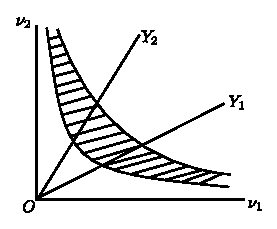
\includegraphics{figure2.eps}
\end{figure}

Under the mapping $W\to q=(q_{1},q_{2},\ldots,q_{n})$ with
$q_{j}=e^{2\pi iW_{j}}(j=1,2,\ldots,n)$ the domain $D$ goes into a
Reinhardt domain $D^{\ast}$ in the $q$-space and $H^{\ast}(q)=H(W)$ is
regular in $D^{\ast}$. If now $q^{\ast}\in D^{\ast}$, we can find a
Reinhardt domain $V$ defined by $a_{k}<|q_{k}|<b_{k}$,
$k=1,2,\ldots,n$ such that $q^{\ast}\in V\in D^{\ast}$. Since
$H^{\ast}(q)$ is regular in $V$, it has a Laurent
expansion\pageoriginale
$\sum\limits_{-\infty<r_{1},\ldots,r_{n}<\infty}c_{r_{1},\ldots,r_{n}}q^{r_{1}}_{1}\ldots
q^{r_{n}}_{n}$ which converges absolutely, uniformly in every compact
subset of $V$. In other words, for $q\in V$, we have
$$
H(W)=H^{\ast}(q)=\sum_{-\infty<r_{1},\ldots,r_{n}<\infty}c_{r_{1},\ldots,r_{n}}e^{2\pi
  i(r_{1}W_{1}+\cdots+r_{n}W_{n})}.
$$
Since $D^{\ast}$ is a Reinhardt domain, it is possible to continue
$H^{\ast}(q)$ analytically from $q^{\ast}$ to any point $q\in
D^{\ast}$ through a finite chain of overlapping Reinhardt domains of
the type of $V$ and if, in addition, we use the fact that the Laurent
expansion is unique, we see that for all $W\in D$, 
\begin{equation*}
H(W)=\sum_{-\infty<r_{1},\ldots,r_{n}<+\infty}c_{r_{1},\ldots,r_{n}}e^{2\pi
  i(r_{1}W_{1}+\cdots+r_{n}W_{n})},\tag{159}\label{159} 
\end{equation*}
the series converging absolutely, uniformly over every compact subset
of $D$.

We can find $\beta_{1},\ldots,\beta_{n}$ in $K$ such that
$S(\alpha_{i}\beta_{j})=\delta_{ij}$ (the Kronecker symbol), for $i$,
$j=1,2,\ldots,n$. Then $\beta_{1},\ldots,\beta_{n}$ constitute a
minimal basis of $\mathfrak{a}^{2}\vartheta^{-1}$ and when
$r_{1},\ldots,r_{n}$ run over all rational integers from $-\infty$ to
$+\infty$ independently, $\beta=r_{1}\beta_{1}+\cdots+r_{n}\beta_{n}$
runs over all numbers of the ideal
$\mathfrak{a}^{2}\vartheta^{-1}$. We shall denote
$c_{r_{1},\ldots,r_{n}}$ by $c(\beta)$. Now
$W_{k}=\sum\limits^{n}_{i=1}\beta^{(i)}_{k}w_{i}$, $k=1,2,\ldots,n$,
as can be easily verified. We then see from \eqref{159} that when $w$
lies in the region $v_{1}>0,\ldots,v_{n}>0$, $R^{-2}<v_{1}\ldots
v_{n}<r^{-2}$, we have
\begin{equation*}
G(w)=H(W)=\sum_{\beta\in
  \mathfrak{a}^{2}\vartheta^{-1}}c(\beta)e^{2\pi iS(\beta
  w)}.\tag{160}\label{160} 
\end{equation*}

If $\epsilon$ is a unit in $K$, then the transformation $w\to
\epsilon^{2}w$ corresponds to an affine transformation of the
$W$-space which takes $D$ into itself. We therefore have from
\eqref{160} that
$$
G(\epsilon^{2}w)=\sum_{\beta\in
  \mathfrak{a}^{2}\vartheta^{-1}}c(\beta)e^{2\pi
  iS(\beta\epsilon^{2}w)}.
$$
On the other hand, from \eqref{158} and \eqref{160},
$$
G(\epsilon^{2}w)=N(\epsilon)^{k}\sum_{\beta\in\mathfrak{a}^{2}\vartheta^{-1}}c(\beta)e^{2\pi
  iS(\beta w)}. 
$$\pageoriginale
For $\beta\in\mathfrak{a}^{2}\vartheta^{-1}$, $\beta\epsilon^{2}$ is
also in $\mathfrak{a}^{2}\vartheta^{-1}$. On comparing the Fourier
coefficients of $G(\epsilon^{2}w)$, we obtain
$$
c(\beta\epsilon^{2})=N(\epsilon)^{-k}c(\beta),
$$
\ie
$$
|c(\beta\epsilon^{2})|=|c(\beta)|.
$$
Thus
$$
|c(\beta\epsilon^{2m})|=|c(\beta)|\text{ for any rational integer } m.
$$

Let us consider a unit cube $U$ in $D$, defined as the set of
$W=(W_{1},\ldots,W_{n})$, $W_{j}=X_{j}+iY^{\ast}_{j}$ and $0\leq
X_{j}\leq 1$. Further let $|H(W)|\leq M$ on $U$. From \eqref{159}, we
have for $\beta=r_{1}\beta_{1}+\cdots+r_{n}\beta_{n}$,
\begin{multline*}
c(\beta)=c_{r_{1},\ldots,r_{n}}=\mathop{\int\ldots\int}\limits_{W\in
  U} H(W)e^{-2\pi i(r_{1}W_{1}+\cdots+r_{n}W_{n})}dX_{1}\ldots
dX_{n}\\
=e^{2\pi S(\beta
  v^{\ast})}\mathop{\int^{1}_{0}\ldots\int^{1}_{0}}\limits_{W\in U}
H(W)e^{-2\pi i(r_{1}X_{1}+\cdots+r_{n}X_{n})}dX_{1}\ldots dX_{n}, 
\end{multline*}
\ie
$$
|c(\beta)|\leq e^{2\pi S(\beta v^{\ast})}M,
$$
where $v^{\ast}=(v^{\ast}_{1},\ldots,v^{\ast}_{n})$ with
$v^{\ast}_{j}=\sum\limits^{n}_{i=1}\alpha^{(j)}_{i}Y^{\ast}_{i}>0$.

Taking $\beta\epsilon^{2m}$ instead of $\beta$, we have
$$
|c(\beta\epsilon^{2m})|\leq e^{2\pi S(\beta\epsilon^{2m}v^{\ast})}M,
$$
\ie
\begin{equation*}
|c(\beta)|\leq e^{2\pi S(\beta\epsilon^{2m}v^{\ast})}M.\tag{161}\label{161}
\end{equation*}

Let now $\beta\in \mathfrak{a}^{2}\vartheta^{-1}$ with $\beta^{(i)}<0$
for some $i$. We claim that $c(\beta)=0$, necessarily. For, using the
existence of $n-1(n\geq 2!)$ independent units in $K$ we can find a
unit $\epsilon$ in $K$ such that
$$
|\epsilon^{(i)}|>1,|\epsilon^{(j)}|<1\text{ \ for \ } j\neq i.
$$\pageoriginale 
Then, as $m$ tends to infinity, $S(\beta\epsilon^{2m}v^{\ast})$ tends
to $-\infty$. Hence, from \eqref{161}, we see that unless $\beta>0$ or
$\beta=0$, $c(\beta)=0$. Thus
$$
G(w)=c(0)+\sum_{\mathfrak{a}^{2}\vartheta^{-1}|\beta>0}c(\beta)e^{2\pi
  iS(\beta w)},
$$
\ie
\begin{equation*}
f(z)N(-\sigma
z+\rho)^{k}=c(0)+\sum_{\mathfrak{a}^{2}\vartheta^{-1}|\beta>0}c(\beta)e^{2\pi
  iS(\beta z_{A^{-1}})},\tag{162}\label{162} 
\end{equation*}
where the series on the right hand side converges absolutely,
uniformly in every compact subset of the region
$r<\Delta(z,\lambda)<R$.

Let now $0<\Delta(z,\lambda)\leq r$ \ie $r^{-2}\leq
N(y_{A^{-1}})<\infty$. We can then find a number $t$ with $0<t<1$ such
that $R^{-2}<N(ty_{A^{-1}})<r^{-2}$. Hence the series
$c(0)+\sum\limits_{\mathfrak{a}^{2}\vartheta^{-1}|\beta>0}c(\beta)e^{2\pi
  iS(\beta wt)}$ converges absolutely. Now, since
$$
c(0)+\sum_{\mathfrak{a}^{2}\vartheta^{-1}|\beta>0}c(\beta)e^{2\pi
  iS(\beta w)}\leq |c(0)|+\sum_{\beta}|c(\beta)||e^{2\pi iS(t\beta
  w)}|,
$$
it converges absolutely. It is now clear that the series on the right
hand side of \eqref{162} converges absolutely, uniformly over every
compact subset in $\mathfrak{H}_{n}$ for which
$0<\Delta(z,\lambda)\leq r$ and provides the analytic continuation of
$f(z)N(-\sigma z+\rho)^{+k}$ in $0<\Delta(z,\lambda)<R$. Thus $f(z)$
is regular in the full neighbourhood $0<\Delta(z,\lambda)<R$, of the
cusp $\lambda$ and moreover, in this neighbourhood,
\begin{equation*}
f(z)N(-\sigma
z+\rho)^{k}=c(0)+\sum_{\mathfrak{a}^{2}\vartheta^{-1}|\beta>0}c(\beta)e^{2\pi
  iS(\beta z_{A^{-1}})}.\tag{163}\label{163}
\end{equation*}

From the theorem above, we can deduce two important corollaries.

\begin{itemize}
\item[(a)] {\em Let $V_{i}$ denote the neighbourhood
  $0<\Delta(z,\lambda_{i})<d_{i}<c$ of the cusp
  $\lambda_{i}(i=1,2,\ldots,h)$ of $\mathfrak{F}$ and let
  $\mathfrak{F}^{\ast}=\mathfrak{F}-\bigcup\limits^{h}_{i=1}V_{i}$. Then
  a function $f(z)$ which is regular in $\mathfrak{F}^{\ast}$ and
  satisfies \eqref{157} for all $M\in\Gamma$ is automatically regular
  in the whole of $\mathfrak{F}$ and hence in the whole of
  $\mathfrak{h}_{n}$ and is an entire modular form, for $n\geq 2$.}

\item[(b)] {\em For $n\geq 2$, if a function $f(z)$ satisfies
  conditions $(1)$ and $(2)$ in the definition\pageoriginale of a
  modular form, it satisfies condition $(3)$ automatically and is
  therefore regular at the cusp $\mathfrak{F}$.}
\end{itemize}

The proofs of (a) and (b) are very simple, in view of Theorem
\ref{thm17}.

The second of the two results above was first proved by Gotzky in the
special case $n=2$ and $K=\bQ(\sqrt{5})$, the class number $h$ being
$1$. In the general case, it was proved by Gundlach. An analogue of
this result in the case of modular forms of degree $n$ was established
by Koecher.

In the theorem above, we might, instead of $\mathfrak{H}_{n}$, take,
for example, the space $\mathfrak{H}^{\ast}_{n}$ of
$(z_{1},\ldots,z_{n})\in C^{n}$ with $\Iim(z_{1})<0$,
$\Iim(z_{2})>0,\ldots,\Iim(z_{n})>0$.  Then, under the same conditions
as in the theorem above, we have for $f(z)N(-\sigma z+\rho)^{k}$ an
expansion of the form
$c(0)+\sum\limits_{\mathfrak{a}^{2}\vartheta^{-1}|\beta>0}c(\beta)e^{2\pi
  iS(\beta z_{A^{-1}})}$, where $\beta$ runs over all numbers of
$\mathfrak{a}^{2}\vartheta^{-1}$ for which $\beta^{(1)}<0$,
$\beta^{(2)}>0,\ldots,\beta^{(n)}>0$. For other types of such spaces
again we have similar expansions for $f(z)N(-\sigma z+\rho)^{k}$ at
the cusp $\rho/\sigma$.

So far, there was no restriction on $k$ except that $k$ should be
integral and $kn$ should be even. In view of the following proposition
however, we shall henceforth be interested only in modular forms of
weight $k>0$.

\begin{proposition}\label{prop24}
A modular form of weight $k<0$ vanishes identically and the only
modular forms of weight $0$ are constants.
\end{proposition}

\begin{proof}
First, let $f(z)$ be a modular form of weight $k<0$. Consider
$\varphi(z)=N(y)^{k/2}|f(z)|$ for $z=x+iy\in\mathfrak{H}_{n}$. We
shall prove that $\varphi(z)$ is bounded in the whole of
$\mathfrak{H}_{n}$. Let, in fact, $\lambda_{i}=\rho_{i}/\sigma_{i}$ be
a cusp of $\mathfrak{F}$ and $V_{i}$, the neighbourhood of
$\lambda_{i}$ defined by $0<\Delta(z,\lambda_{i})<d$. Now, since
$N(y)^{k/2}=N(y_{A^{-1}_{i}})^{k/2}|N(-\sigma_{i}z+\rho_{i})|^{k}$, we
have
\begin{equation*}
\varphi(z) = N(y_{A^{-1}_{i}})^{k/2}|f(z) ||
N(-\sigma_{i}z+\rho_{i})|^{k}
.\tag{164}\label{164}  
\end{equation*}
Further, from \eqref{163},
$$
f(z)N(- \sigma_{i} z +
\rho_{i})^{k} = c_{i}(0) + \sum_{\mathfrak{a}^{2} \vartheta^{-1}
  |\beta>0}c_{i}(\beta)e^{2\pi  
  iS(\beta z_{A^{-1}_{i}})} 
$$
and clearly for $z\in V_{i}\cap \mathfrak{F}$,
$f(z)N(-\sigma_{i}z+\rho_{i})^{k}$ is bounded. Moreover, since for
$z\in V_{i}$, $N(y_{A^{-1}_{i}})^{k/2}<d^{-k}$, we conclude from
\eqref{164} that $\varphi(z)$ is bounded\pageoriginale in
$\bigcup\limits^{h}_{i=1}(V_{i}\cap \mathfrak{F})$. Let
$\mathfrak{F}^{\ast}=\mathfrak{F}-\bigcup\limits^{h}_{i=1}(V_{i}\cap\mathfrak{F})$. Since
$\mathfrak{F}^{\ast}$ is compact, $\varphi(z)$ is bounded on
$\mathfrak{F}^{\ast}$. Thus there exists a constant $M$ such that
$\varphi(z)\leq M$ for $z\in\mathfrak{F}$. But now for each
$P=\left(\begin{smallmatrix} \alpha & \beta\\ \gamma & \delta 
\end{smallmatrix}\right)\in\Gamma$, $\varphi(z_{P})=\varphi(z)$, since
\begin{align*}
|f(z_{P})|N(y_{P})^{k/2} &= |f(z_{P})||N(\gamma
z+\delta)|^{-k}N(y)^{+k/2}=|f(z)|N(y)^{k/2}\\
&=\varphi(z). 
\end{align*}
Thus, for all $z\in \mathfrak{h}_{n}$, $\varphi(z)\leq M$ and hence
\begin{equation*}
\begin{aligned}
|f(z)| &= \varphi(z)N(y)^{-k/2}\\
&\leq MN(y)^{-k/2}.
\end{aligned}\tag{165}\label{165}
\end{equation*}
Now
$$
f(z)=c(0)+\sum_{\vartheta^{-1}|\beta \succ 0}c(\beta)e^{2\pi iS(\beta z)}
$$
and
\begin{align*}
c(\alpha) &= \int^{1}_{0}\ldots\int^{1}_{0}f(z)e^{-2\pi iS(\alpha
  z)}dx_{1}\ldots dx_{n}\\
&= e^{2\pi S(\alpha y)}\int^{1}_{0}\ldots\int^{1}_{0}f(x+iy)e^{-2\pi
  iS(\alpha x)}dx_{1}\ldots dx_{n}.
\end{align*}
Hence, from \eqref{165},
$$
|c(\alpha)|\leq MN(y)^{-k/2}e^{2\pi S(\alpha y)}
$$
Letting $y$ tend to $(0,\ldots,0)$ and noting that $k<0$, we see that
$c(\alpha)=0$ for all $\alpha\in\vartheta^{-1}$ and hence $f(z)$ is
identically zero.
\end{proof}

Let now $\psi(z)$ be a modular form of weight $0$. For each cusp
$\lambda_{i}$ of $\mathfrak{F}$, we have
$$
\psi(z)=c_{i}(0)+\sum_{\mathfrak{a}^{2}_{i}\vartheta^{-1}|\beta \succ
  0}c_{i}(\beta)e^{2\pi 
  iS(\beta z_{A^{-1}_{i}})}.
$$
Consider $\chi(z)=\prod\limits^{h}_{i=1}(\psi(z)-c_{i}(0))$. Let, if
possible, $\chi(z)$ be not identically zero \ie for
$z_{0}\in\mathfrak{F}$, let $|\chi(z_{0})|=\rho\neq 0$. Since
$\psi(z)-c_{i}(0)$ tends to zero\pageoriginale as $z$ tends to
$\lambda_{i}$ in $\mathfrak{F}$, we can find a neighbourhood $V_{i}$
of $\lambda_{i}$ such that for $z\in V_{i}\cap \mathfrak{F}$,
$|\chi(z)|<(1/2)\rho$. Now
$\mathfrak{F}^{\ast}=\mathfrak{F}-\bigcup\limits^{h}_{i=1}(V_{i}\cap
\mathfrak{F})$ is compact and $|\chi(z)|$ attains its maximum $M$ at
some point of $\mathfrak{F}^{\ast}$. We see easily that
$$
M=\max\limits_{z\in\mathfrak{F}}|\chi(z)|=\max\limits_{z\in
  \mathfrak{h}_{n}}|\chi(z)|. 
$$
But his means that $\chi(z)$ attains its maximum modulus over
$\mathfrak{H}_{n}$ at an inner point of $\mathfrak{H}_{n}$ and by the
maximum principle, $\chi(z)$ is a constant. But now, since $\chi(z)$
tends to zero as $z$ tends to the cusps of $\mathfrak{F}$, $\chi(z)=0$
identically in $\mathfrak{H}_{n}$. This means that
$\prod\limits^{h}_{i=1}(\psi(z)-c_{i}(0))=0$. Since $\psi(z)$ is
single-valued and regular in $\mathfrak{H}_{n}$, it follows that
$\chi(z)$ is a constant.

Our object now is to give an explicit construction of modular forms of
weight $k>2$ ($k$ being integral). Our method will involve an
adaptation of the well-known idea of Poincare for constructing
automorphic forms belonging to a discontinuous group $\Gamma_{0}$ of
analytic automorphisms of the unit disc $D$ defined by $|z|<1$ in the
complex $z$-plane. Now, any analytic automorphism of $D$ is given by
the mapping $z\to \dfrac{\ob{a}z+\ob{b}}{bz+a}$, where $a$ and $b$ are
complex numbers satisfying $|a|^{2}-|b|^{2}=1$. Let the elements of
$\Gamma_{0}$ be $M_{i}=\left(\begin{smallmatrix} \ob{a}_{i} &
  \ob{b}_{i}\\ b_{i} & a_{i}\end{smallmatrix}\right)$, $i=1,2,\ldots$
(corresponding to the automorphisms $z\to
z_{M_{i}}=\dfrac{\ob{a}_{i}z+\ob{b}_{i}}{b_{i}z+a_{i}}$ of $D$).

Let $z_{0}$ be a given point of $D$. Now, since $\Gamma_{0}$ acts
discontinuously on $D$, we can find a neighbourhood $V$ of $z_{0}$
such that the images $V_{M}$ of $V$ for $M\in \Gamma_{0}$ do not
intersect $V$, unless $(z_{0})_{M}=z_{0}$. Let $n_{0}$ be the order of
the isotropy group of $z_{0}$ in $\Gamma_{0}$. Then we see that
$$
\sum_{M\in\Gamma_{0}}\iint\limits_{V_{M}}dx\ dy\leq n_{0}\cdot \pi.
$$
On the other hand, for $M=\left(\begin{smallmatrix} \ob{a} &
  \ob{b}\\ b & a\end{smallmatrix}\right)\in\Gamma_{0}$, we have
$$
\iint\limits_{V_{M}}dx\ dy =\iint\limits_{V}|bz+a|^{-4}dx\ dy.
$$
Therefore,\pageoriginale
\begin{equation*}
\sum_{M\in\Gamma_{0}}\iint\limits_{V}|bz+a|^{-4}dx\ dy\leq n_{0}\cdot
\pi.\tag{166}\label{166} 
\end{equation*}
Since $|a|^{2}-|b|^{2}=1$, $a\neq 0$ and further $|b/a|<1$. Hence, for
$z\in D$,
\begin{equation*}
1-|z|\leq \left|\frac{bz+a}{a}\right|<1+|z|.\tag{167}\label{167}
\end{equation*}
Let $V$ be contained in the disc $|z|\leq r<1$ and let $v$ denote the
area of $V$. We have, then, in view of \eqref{166} and \eqref{167},
\begin{equation*}
v(1+r)^{-4}\sum_{M\in\Gamma_{0}}|a|^{-4}\leq
\sum_{M\in\Gamma_{0}}\iint\limits_{V} |bz+a|^{-4}dx\ dy\leq n_{0}\cdot
\pi.\tag{168}\label{168} 
\end{equation*}

We conclude that $\sum\limits_{M\in\Gamma_{0}}|a|^{-4}$ is
convergent. Further, from \eqref{167}, we have for $z\in V$,
$$
\sum_{M\in\Gamma_{0}}|bz+a|^{-4}<(1-r)^{-4}\sum_{M\in\Gamma_{0}}|a|^{-4}
$$
Hence $\sum\limits_{M\in\Gamma_{0}}(bz+a)^{-4}$ converges absolutely,
uniformly on every compact subset of $V$. Since $z_{0}$ is arbitrary,
this is true even for every compact subset of $D$.

Using the same idea as above, we shall prove that actually
$\sum\limits_{M\in\Gamma_{0}}(bz+a)^{-k}$ converges absolutely for
$k>2$. Consider
$$
I_{l}=\iint\limits_{V}\frac{dx\ dy}{(1-|z|^{2})^{l}};
$$
the integral converges if and only if $l<1$. Now, as before
$$
\sum_{M}\iint\limits_{V_{M}}\frac{dx\ dy}{(1-|z|^{2})^{-l}}\leq
n_{0}I_{l}. 
$$
But 
$$
\iint\limits_{V_{M}}\frac{dx\ dy}{(1-|z|^{2})^{l}}=\iint\limits_{V}|bz+a|^{-4+2l}\frac{dx\ dy}{(1-|z|^{2})^{l}}\text{ 
  \  for \ } M=
\begin{pmatrix}
\ob{a} & \ob{b}\\
b & a
\end{pmatrix}
\in\Gamma_{0}.
$$
Thus\pageoriginale
$$
\sum_{M\in\Gamma_{0}}\iint\limits_{V}|bz+a|^{2l-4}\frac{dx\ dy}{(1-|z|^{2})^{l}}=\sum_{M}\iint\limits_{V_{M}}\frac{dx\ dy}{(1-|z|^{2})^{l}}\leq
n_{0}I_{l}. 
$$

Using the same argument as earlier, it is easily shown that
$\sum\limits_{M\in\Gamma_{0}}(bz+a)^{-4+2l}$ and therefore
$\sum\limits_{M\in\Gamma_{0}}(bz+a)^{-k}$, (for $k>2$) converges
absolutely, uniformly on every compact subset of $D$.

Let $k$ be an even rational integer {\em greater than } 2. Then we see
that $\psi(z,k)=\sum\limits_{M\in\Gamma_{0}}(bz+a)^{-k}$ is analytic
in $D$. To verify that $\psi(z,k)$ is an automorphic form belonging to
$\Gamma_{0}$, we have only to show that
$$
\text{for \ } N=
\begin{pmatrix}
\ob{p} & \ob{q}\\
q & p
\end{pmatrix}
\in\Gamma_{0},\psi(z_{N},k)(qz+p)^{-k}=\psi(z,k).
$$
Now, for
$$
M=
\begin{pmatrix}
\ob{a} & \ob{b}\\
b & a
\end{pmatrix}
\in \Gamma_{0}, \left(\frac{dz_{M}}{dz}\right)^{k/2}=(bz+a)^{-k}
$$
and so 
$$
\psi(z,k)=\sum_{M\in\Gamma_{0}}\left(\frac{dz_{M}}{dz}\right)^{k/2}
$$
Further
\begin{align*}
\psi(z_{N},k) &=
\sum_{M\in\Gamma_{0}}\left(\frac{dz_{MN}}{dz_{N}}\right)^{k/2}\\
&=
\left(\frac{dz_{N}}{dz}\right)^{-k/2}\sum_{M\in\Gamma_{0}}\left(\frac{dz_{MN}}{dz}\right)^{k/2}\\
&= (qz+p)^{k}\psi(z,k),
\end{align*}
since $MN$ runs over all elements of $\Gamma_{0}$, when $M$ does
so. Thus $\psi(z,k)$ is an automorphic form of weight $k$, for the
group $\Gamma_{0}$ and is a so-called {\bf Poincar\'e series} of
weight $k$ for $\Gamma_{0}$.

The\pageoriginale method given above for the construction of
automorphic forms for the group $\Gamma_{0}$ is due to Poincar\'e and
it cannot be carried over as such to the case of the Hilbert modular
group, since the euclidean volume of $\mathfrak{H}_{n}$ is
infinite. In the following, we shall give a method of constructing
Hilbert modular forms of weight $k>2$, based on a slight modification
of the idea of Poincar\'e. We shall be interested only in the case
$n\geq 2$.

Let $\lambda=\rho/\sigma$ be a cusp of $\mathfrak{H}_{n}$,
$\mathfrak{a}=(\rho,\sigma)=\mathfrak{a}_{i}$ (for some $i$),
$A=\left(\begin{smallmatrix} \rho & \xi\\ \sigma & \eta
\end{smallmatrix}\right)\in\mathfrak{S}$ associated with $\lambda$ and
$z_{A^{-1}}=z^{\ast}=x^{\ast}+iy^{\ast}$. We had introduced in
$\mathfrak{H}_{n}$ a system of `local coordinates' relative to the
cusp $\lambda$, namely, $N(y^{\ast})^{-\frac{1}{2}}$,
$Y_{1},\ldots,Y_{n-1}$, $X_{1},\ldots,X_{n}$. Defining
$q=N(y^{\ast})$, it is easily seen that the relationship between the
volume element $dv=dq$, $dY_{1},\ldots,dY_{n-1}$,
$dX_{1},dX_{2},\ldots,dX_{n}$ and the ordinary euclidean volume
element $dx_{1}dy_{1},\ldots,dx_{n}dy_{n}$ in $\mathfrak{H}_{n}$ is
given by
$$
dv=\frac{N(\mathfrak{a})^{2}}{2^{n-1}R_{0}\sqrt{|d|}}|N(-\sigma
z+\rho)|^{-4}dx_{1}dy_{1},\ldots,dx_{n}dy_{n}, 
$$
where $R_{0}$ and $d$ are respectively the regulator and the
discriminant of $K$. Let now
$$
c=\frac{N(\mathfrak{a})^{2}}{2^{n-1}R_{0}\sqrt{|d|}}
$$
and let $d\omega$ be the volume element
$N(y)^{-2}dx_{1}dy_{1},\ldots,dx_{n}dy_{n}$. Then $d\omega$ is
invariant under a (modular) substitution $z\to z_{M}$ for $M\in\Gamma$
and moreover
$$
dv=c\cdot N(y^{\ast})^{2}d\omega=c\Delta(z,\lambda)^{-4}d\omega.
$$
Now, under the transformation $z\to z_{M}$ for $M\in\Gamma$, it may be
verified that
\begin{align*}
dv &\to
c\Delta(z_{M},\lambda)^{-4}d\omega=\frac{\Delta(z,\lambda)^{4}}{\Delta(z,\lambda_{M^{-1}})^{4}},
dv, \tag{169}\label{169}\\
N(y^{\ast}) &= \Delta(z,\lambda)^{-2}\to \Delta(z_{M},\lambda)^{-2}=\Delta(z,\lambda_{M^{-1}})^{-2}.
\end{align*}
We can find a point $z_{0}\mathfrak{U}\mathfrak{a}_{\lambda,d}$ such
that $z_{0}$ is not a fixed point of any modular\pageoriginale
transformation except the identity. Now, by Theorem \ref{thm16} again,
we can find a neighbourhood $V$ of $z_{0}$ contained in
$\mathfrak{U}_{\lambda,d}\cap \mathfrak{G}_{\lambda}$ such that $V\cap
V_{M}=\emptyset$, except for $M=\left(\begin{smallmatrix} 1 & 0\\ 0 &
  1\end{smallmatrix}\right)$ in $\Gamma$. Let
  $M_{1}=\left(\begin{smallmatrix} 1 & 0\\ 0 & 1
  \end{smallmatrix}\right)$, $M_{2},\ldots$, be a complete system of
  representatives of the right cosets of $\Gamma$ modulo
  $\Gamma_{\lambda}$. For $i\neq 1$, $M_{i}$ takes
  $\mathfrak{U}_{\lambda,d}$ into $\mathfrak{U}_{\mu,d}$ where
  $\mu=\lambda_{M_{i}}\neq \lambda$ and since
  $\mathfrak{U}_{\lambda,d}\cap \mathfrak{U}_{\mu,d}=\emptyset$, we
  see that for $i\neq 1$, $V_{M_{i}}$ lies wholly outside the
  neighbourhood $\mathfrak{U}_{\lambda,d}$. Further $V_{M_{i}}\cap
  V_{M_{j}}=\emptyset$ unless $M_{i}=M_{j}$. Now, by applying suitable
  transformations in $\Gamma_{\lambda}$ to the images $V_{M_{i}}$ or
  parts of the same, we might suppose that $V_{M_{i}}\subset
  \mathfrak{G}_{\lambda}$ for all $i$. It is to be remarked that under
  this process, the sets $V_{M_{i}}$ continue to have finite euclidean
  volume and to be mutually non-intersecting. Let now, for a suitable
  $d_{0}>0$, $V\subset
  \mathfrak{U}_{\lambda,d}-\mathfrak{U}_{\lambda,d_{0}}$. We then see
  that the mutually disjoint sets $V_{M_{i}}$, $i=1,2,\ldots,$ are all
  contained in
  $\mathfrak{G}_{\lambda}-\mathfrak{U}_{\lambda,d_{0}}$. It is now
  easily verified that
\begin{align*}
J_{s} &=
\sum_{M_{i}}\mathop{\int\ldots\int}_{V_{M_{i}}}N(y^{\ast})^{s-2}dv\\
&\leq
\int^{d_{0}}_{0}\int^{\frac{1}{2}}_{-\frac{1}{2}}\ldots\int^{\frac{1}{2}}_{-\frac{1}{2}}q^{s-2}dq\ dY_{1},\ldots,dY_{n-1}dX_{1},\ldots,dX_{n}\\
&= \int^{d_{0}}_{0}q^{s-2}dq
\end{align*}
and $J_{s}$ converges if and only if $s>1$.

On the other hand, we obtain by \eqref{169}, for
$M=\left(\begin{smallmatrix} \alpha & \beta\\ \gamma &\delta
\end{smallmatrix}\right)\in\Gamma$
$$
\mathop{\int\ldots\int}_{V_{M}}N(y^{\ast})^{s-2}dv=\mathop{\int\ldots\int}_{V}\frac{|N(-\sigma
  z+\rho)|^{4}N(y)^{s-2}}{|N(-\sigma z_{M}+\rho)|^{2s}|N(\gamma
  z+\delta)|^{2s}}dv. 
$$
Now, let
$$
A^{-1}M_{j}=P_{j}=
\begin{pmatrix}
\ast & \ast\\
\gamma_{j} & \delta_{j}
\end{pmatrix},\quad 
j=1,2,\ldots
$$
Then $P_{j}$ runs over a complete set of matrices of the form
$A^{-1}M$ with $M\in\Gamma$ such that for $i\neq j$, $P_{i}\neq
NP_{j}$ with $N\in A^{-1}\Gamma_{\lambda}A$. Equivalently, we see that
$(\gamma_{j},\delta_{j})$ runs over a complete set of non-associated
pairs of integers $\gamma_{j}$, $\delta_{j}$ in $\mathfrak{a}$ such
that $(\gamma_{j},\delta_{j})=\mathfrak{a}$. Now 
\begin{align*}
J_{s} &=
\sum_{M_{i}}\mathop{\int\ldots\int}_{V_{M}}N(y^{\ast})^{s-2}dv\\
&=
\mathop{{\sum}'}_{\gamma_{j},\delta_{j}}\mathop{\int\ldots\int}_{V}|N(\gamma_{j}z+\delta_{j})|^{-2s}|N(-\sigma z+\rho)|^{2s}N(y^{\ast})^{s-2}dv
\end{align*}\pageoriginale
where on the right hand side, the summation is over a complete set of
non-associated pairs of integers $(\gamma_{j},\delta_{j})$ such that
$(\gamma_{j},\delta_{j})=\mathfrak{a}$.

Let $B$ be a compact set in $\mathfrak{H}_{n}$. We can then find
constants $c_{13}$ and $c_{14}$ depending only on $B$ such that for
all  $z\in B$ and real $\mu$ and $\nu$, we have
\begin{equation*}
c_{13}|N(\mu j+\nu)|\leq |N(\mu z+\nu)|\leq c_{14}|N(\mu
j+\nu)|.\tag{170}\label{170} 
\end{equation*}
Taking for $B$, the closure $\ob{V}$ and $V$ in $\mathfrak{H}_{n}$, we
see that for a suitable constant $c_{15}$ depending only on $V$ and
for $s>1$,
$$
\mathop{{\sum}'}_{\gamma_{j},\delta_{j}}|N(\gamma_{j}i+\delta_{j})|^{-2s}\leq
c_{15}J_{s}<\infty.
$$

Let now $z$ lie in an arbitrary compact set $B$ in
$\mathfrak{H}_{n}$. Then, in view of \eqref{170}, we can find a
constant $c_{16}$ depending only on $B$, such that for all $z\in B$,
$$
\mathop{{\sum}'}_{\gamma_{j},\delta_{j}}|N(\gamma_{j}z+\delta_{j})|^{-2s}\leq
c_{16}\mathop{{\sum}'}_{\gamma_{j},\delta_{j}}|N(\gamma_{j}i+\delta_{j})|^{-2s}<\infty.
$$

Thus the series
$\mathop{{\sum}'}\limits_{\gamma_{j},\delta_{j}}N(\gamma_{j}z+\delta_{j})^{-2s}$
converges absolutely, uniformly over every compact subset of
$\mathfrak{H}_{n}$, for $s>1$.

Let $\mathfrak{a}_{1}$ and $\mathfrak{a}_{2}$ denote a full system of
pairs of integers $(\gamma,\delta)$ satisfying
$(\gamma,\delta)=\mathfrak{a}$ and not mutually associated,
respectively with respect to the group of all units in $K$ and the
group of units of norm $1$ in $K$.

Let $k$ be a rational integer greater than $2$. Corresponding to an
integral ideal $\mathfrak{a}$ in $K$, we now define for
$z\in\mathfrak{H}_{n}$, the function
$$
G^{\ast}(z,k,\mathfrak{a})=\sum_{(\gamma^{\ast},\delta^{\ast})\in\mathfrak{a}_{2}}N(\gamma^{\ast}z+\delta^{\ast})^{-k}.
$$
We first observe that $G^{\ast}(z,k,\mathfrak{a})$ is well-defined and
is independent of the particular\pageoriginale choice of elements of
$\mathfrak{a}_{2}$. Further, since the group of units of norm $1$ in
$K$ is of index at most $2$ in the group of all units in $K$. We
deduce from the foregoing considerations that the series
$\sum\limits_{(\gamma^{\ast},\delta^{\ast})\in\mathfrak{a}_{2}}N(\gamma^{\ast}z+\delta^{\ast})^{-k}$ 
converges absolutely uniformly over any compact subset of
$\mathfrak{H}_{n}$. Hence $G^{\ast}(z,k,\mathfrak{a})$ is regular in
$\mathfrak{H}_{n}$. Moreover, for $M=\left(\begin{smallmatrix} \rho &
  x\\ \mu & \nu\end{smallmatrix}\right)\in \Gamma$, 
\begin{align*}
G^{\ast}(z_{M},k,\mathfrak{a}) &=
\sum_{(\gamma^{\ast},\delta^{\ast})\in
  \mathfrak{a}_{2}}N(\gamma^{\ast}z_{M}+\delta^{\ast})^{-k}\\
&= N(\mu
z+\nu)^{k}\sum_{(\gamma^{\ast},\delta^{\ast})\in\mathfrak{a}_{2}}N((\gamma^{\ast}\rho+\delta^{\ast}\mu)z+\gamma^{\ast}x+\delta^{\ast}\nu)^{-k}.  
\end{align*}
Now
$(\gamma^{\ast}\rho+\delta^{\ast}\mu,\gamma^{\ast}x+\delta^{\ast}\nu)$
again runs over a system $\mathfrak{a}_{2}$ when
$(\gamma^{\ast},\delta^{\ast})$ does so. Thus
$$
G^{\ast}(z_{M},k,\mathfrak{a})N(\mu
z+\nu)^{-k}=G^{\ast}(z,k,\mathfrak{a}).
$$
Therefore $G^{\ast}(z,k,\mathfrak{a})$ is a modular form of weight
$k$.

Let $k$ be odd and $K$ contain a unit $\epsilon_{0}$ of norm $-1$; for
example, if the degree $n$ is odd, then $-1$ has norm $-1$. If
$(\gamma,\delta)$ runs over a system $\mathfrak{a}_{1}$, then
$(\gamma,\delta)$ together with
$(\epsilon_{0}\gamma,\epsilon_{0}\delta)$ runs over a system
$\mathfrak{a}_{2}$. Thus
$$
G^{\ast}(z,k,\mathfrak{a})=(1+N(\epsilon_{0})^{k})\sum_{(\gamma,\delta)\in\mathfrak{a}_{1}}N(\gamma
z+\delta)^{-k}=0, 
$$
since $N(\epsilon_{0})^{k}+1=0$. Thus the function
$G^{\ast}(z,k,\mathfrak{a})$ vanishes identically in the case when $k$
is odd and $K$ contains a unit of norm $-1$. We shall {\em henceforth}
exclude this case from our consideration; in particular, $nk$ should
necessarily be even. We have then
$$
G^{\ast}(z,k,\mathfrak{a})=\rho G(z,k,\mathfrak{a}),
$$
where, by definition
$$
G(z,k,\mathfrak{a})=\sum_{(\gamma,\delta)\in\mathfrak{a}_{1}}N(\gamma
z+\delta)^{-k} 
$$
and $\rho$ is the index of the group of units of norm $1$ in $K$ in
the group of all units in $K$. The functions $G(z,k,\mathfrak{a})$ are
again modular forms of weight $k$ and are the so-called {\bf
  Eisenstein series} for the Hilbert modular group.

If\pageoriginale $\mathfrak{a}=(\mu)\mathfrak{a}_{i}$ for some
$i(=1,2,\ldots h)$ and $\mu\in K$, then
$G(z,k,\mathfrak{a})=N(\mu)^{-k}G(z,k,\mathfrak{a}_{i})$. For the sake
of brevity, we may denote $G(z,k,\mathfrak{a}_{i})$ by $G_{i}(z,k)$
for $i=1,2,\ldots,h$.

We can obtain the Fourier expansion of $G_{i}(z,k)$ at the various
cusps $\lambda_{j}$ of $\mathfrak{F}$ (\cf formula \eqref{163} above)
by using the following generalized `Lipschitz formula' valid for
rational integral $s>2$ and $\tau \in\mathfrak{H}_{n}$, namely, 
\begin{equation*}
\sum_{\substack{\zeta\text{ integral}\\ \zeta\in
    K}}N(\tau+\zeta)^{-s}=\frac{\left(\dfrac{2\pi}{i}\right)^{ns}}{\sqrt{N(\vartheta)}(\Gamma(s))^{n}}\sum_{\substack{\mu\in\vartheta^{-1}\\ \mu>0}}(N(\mu))^{s-1}e^{2\pi
  S(\mu\tau)}.\tag{171} \label{171}
\end{equation*}
But we shall not go into the details here.

A modular form $f(z)$ is said to {\em vanish at a cusp}
$\lambda=\rho/\sigma$ of $\mathfrak{H}_{n}$, if, in the Fourier
expansion of $f(z)N(-\sigma z+\rho)^{k}$ at the cups $\lambda$ (\cf
formula \eqref{163}), the constant term $c(0)$ is zero. If $f(z)$
vanishes at a cusp $\lambda$, it clearly vanishes at all the
equivalent cusps.

We shall now prove the following

\begin{proposition}\label{prop25}
The Eisenstein series $G_{i}(z,k)(k>2)$ vanishes at all cusps of
$\mathfrak{H}_{n}$ except at those equivalent to $\lambda_{i}$.
\end{proposition}

\begin{proof}
Let $\lambda_{j}=\rho_{j}/\sigma_{j}$ be a base cusp of $\mathfrak{F}$
and $A_{j}=\left(\begin{smallmatrix} \rho_{j} & \xi_{j}\\ \sigma_{j} &
  \eta_{j}\end{smallmatrix}\right)$ be the associated matrix in
$\mathfrak{S}$. Then setting $w=z_{A^{-1}_{j}}$, we have
$$
G_{i}(z,k)N(-\sigma_{j}z+\rho_{j})^{k}=\mathop{{\sum}'}_{(\gamma,\delta)=\mathfrak{a}_{i}}N((\gamma\rho_{j}+\delta\sigma_{j})w+\gamma\xi_{j}+\delta\eta_{j})^{-k}.
$$
Let us denote by $c_{ij}$ the constant term in the Fourier expansion
of $G_{i}(z,k)\break N(-\sigma_{j}z+\rho_{j})^{k}$ at the cusp
$\lambda_{j}$. If we set $w=(\sqrt{-1}t,\ldots\sqrt{-1}t)(t>0)$, then
\begin{align*}
c_{ij} &= \lim\limits_{t\to
  \infty}G_{i}(z,k)N(-\sigma_{j}z+\rho_{j})^{k}\\
&= \lim\limits_{t\to
  \infty}\mathop{{\sum}'}_{(\gamma,\delta)=\mathfrak{a}_{i}}N((\gamma\rho_{j}+\delta\sigma_{j})\sqrt{-1}t+\gamma\xi_{j}+\delta\eta_{j})^{-k}\\
&=
\mathop{{\sum}'}_{(\gamma,\delta)=\mathfrak{a}_{i}}\lim\limits_{t\to
  \infty}N((\gamma\rho_{j}+\delta\sigma_{j})\sqrt{-1}t+\gamma\xi_{j}+\delta\eta_{j})^{-k},\tag{172}\label{172} 
\end{align*}
since the interchange of the limit and the summation can be easily
justified.\pageoriginale Now unless
$\gamma\rho_{j}+\delta\sigma_{j}=0$, the corresponding term in the
series \eqref{172} is zero. If $\gamma\rho_{j}+\delta\sigma_{j}=0$,
then
$$
\frac{(\gamma)}{\mathfrak{a}_{i}}\frac{(\rho_{j})}{\mathfrak{a}_{j}}=\frac{(\delta)}{\mathfrak{a}_{i}}\frac{(\sigma_{j})}{\mathfrak{a}_{j}}
$$
and from this, it follows that necessarily $i=j$. Further, if
$\gamma\rho_{j}+\delta\sigma_{j}=0$, it can be easily shown that
$\gamma\xi_{j}+\delta\eta_{j}\neq 0$. Moreover, in the series
\eqref{172}, there can occur only the pair $(\gamma,\delta)$ for which
$\gamma\rho_{j}+\delta\sigma_{j}=0$ and indeed this happens only if
$i=j$. Therefore $c_{ij}=0$, unless $i=j$. Our contention that
$G_{i}(z,k)$ vanishes at all cusps of $\mathfrak{F}$ except at
$\lambda_{i}$ is therefore established.

We deduce that {\em the $h$ Eisenstein series
  $G_{i}(z,k),i=1,2,\ldots,h$ are linearly independent over the field
  of complex numbers.} If
$\sum\limits^{h}_{i=1}\alpha_{i}G_{i}(z,k)=0$, then letting $z$ tend
to cusp $\lambda_{j}$, the relation
$\left(\sum\limits^{h}_{i=1}\alpha_{i}G_{i}(z,k)\right)N(-\sigma_{j}z+\rho_{j})^{k}=0$
gives $\alpha_{j}c_{jj}=0$ \ie $\alpha_{j}=0$. Thus $\alpha_{i}=0$ for
$i=1,2,\ldots,h$. 
\end{proof}

A modular form which vanishes at all the cusps of $\mathfrak{F}$ is
known as a {\em cusp form.}

It is now easy to prove

\begin{proposition}\label{prop26}
For a given modular form $f(z)$ of integral weight $k>2$, we can find
a linear combination $\varphi(z)$ of the Eisenstein series
$G_{i}(z,k)$ such that $f(z)-\varphi(z)$ is a cusp form.
\end{proposition}

\begin{proof}
If $c_{j}(0)$ is the constant term in the Fourier expansion of
$f(z)\break N(-\sigma_{j}z+\rho_{j})^{k}$ at cusp
$\lambda_{j}=\rho_{j}/\sigma_{j}$ of $\mathfrak{F}$, then the function
$\varphi(z)=\sum\limits^{h}_{i=1}c_{i}(0)c^{-1}_{ii}G_{i}(z,k)$
satisfies the requirements of the proposition.
\end{proof}

The method outlined above for constructing modular forms yields only
Eisenstein series but no cusp forms. In order to construct nontrivial
cusp forms of integral weight $k>2$, we proceed as follows.

Let\pageoriginale $\mathfrak{H}^{\ast}_{n}$ denote the set of $z\in
C^{n}$ for which $-z\in\mathfrak{H}_{n}$. Further let
$w=u-iv\in\mathfrak{H}^{\ast}_{n}$. We define for
$z=x+iy\in\mathfrak{H}_{n}$, integral $l$ and integral $k>2$, the
function
\begin{equation*}
\Phi(w,z)=\sum_{M\in\Gamma}N(\gamma
z+\delta)^{-k}N(w-z_{M})^{-l}\tag{173}\label{173} 
\end{equation*}
where $M=\left(\begin{smallmatrix} \alpha & \beta\\ \gamma & \delta
\end{smallmatrix}\right)$ runs over all elements of $\Gamma$. We shall
show that the series \eqref{173} converges absolutely, uniformly for
$z$ and $w$ lying in compact sets in $\mathfrak{H}_{n}$ and
$\mathfrak{H}^{\ast}_{n}$ respectively, provided that $l>2$, $k\geq
4$.

To this end, we choose $z_{0}\in\mathfrak{R}_{1}$ such that $z_{0}$ is
not a fixed point of any $M$ in $\Gamma$, except
$M=\left(\begin{smallmatrix} 1 & 0\\ 0 & 1
\end{smallmatrix}\right)$. We can then find a neighbourhood $V$ of
$z_{0}$ such that the images $V_{M}$ of $V$ for $M\neq
\left(\begin{smallmatrix} 1 & 0 \\ 0 & 1
\end{smallmatrix}\right)$ in $\Gamma$, do not intersect $V$. We may
suppose moreover that for a suitable $d'>0$, if $W$ denotes the
annular neighbourhood of the base cusp $\infty$ defined by
$0<d'<\Delta(z,\infty)<d$, then $V\subset \mathfrak{G}_{\infty}\cap
W$. It will then follow from result (ii) on p.\@ 199 that for
$M\not\in \Gamma_{\infty}$, $V_{M}$ lies outside the neighbourhood
$\mathfrak{U}_{\infty,d}$ and moreover for $M\in\Gamma_{\infty}$,
$V_{M}\subset W$. In other words, for $M\in\Gamma$, the images $V_{M}$
of $V$ are mutually disjoint and further if
$z\in\bigcup\limits_{M\in\Gamma}V_{M}$, then necessarily we have
$\Delta(z,\infty)\geq d'$, \ie $\bigcup\limits_{M\in\Gamma}V_{M}$ is
contained in a region of the form $N(y)<\alpha$, for some $\alpha>0$.

Let us now consider the integral
$$
I(s,l,\alpha)=\mathop{\int\ldots\int}_{N(y)\leq\alpha}N(y)^{s-2}|N(w-z)|^{-l}dv,
$$
where $dv=dx_{1}dy_{1},\ldots,dx_{n}dy_{n}$ and the integral is
extended over the set in $\mathfrak{H}_{n}$ defined by $N(y)\leq
\alpha$. If $s\geq 2$, then trivially
$$
I(s,l,\alpha)\leq
\alpha^{s-2}\mathop{\int\ldots\int}_{\mathfrak{H}_{n}}|N(w-z)|^{-l}dv
$$
\ie
\begin{align*}
I(s,l,\alpha) &\leq
\alpha^{s-2}\mathop{\int\ldots\int}_{\mathfrak{H}_{n}}N((u-x)^{2}+(v+y)^{2})^{-l/2}dv\\
&=
\alpha^{s-2}\int^{\infty}_{0}\ldots\int^{\infty}_{0}N(v+y)^{1-l}dy_{1}\ldots
dy_{n}\\
&\qquad
\int^{\infty}_{-\infty}\ldots\int^{\infty}_{-\infty}N(1+x^{2})^{-l/2}dx_{1}\ldots
dx_{n}\\
&<\infty,
\end{align*}\pageoriginale
provided $l>2$. Now, since the sets $V_{M}$ are mutually disjoint, we
have
$$
\sum_{M\in\Gamma}\mathop{\int\ldots\int}_{V_{M}}N(y)^{k/2-2}|N(w-z)|^{-l}dv\leq
I\left(\frac{k}{2},l,\alpha\right)<\infty, 
$$
if $l>2$, $k\geq 4$. But, on the other hand, for
$M=\left(\begin{smallmatrix} \alpha & \beta\\ \gamma & \delta
\end{smallmatrix}\right)\in\Gamma$,
\begin{align*}
& \mathop{\int\ldots\int}_{V_{M}}N(y)^{k/2-2}(N(w-z))^{-l}dv\\
& \quad
  =\mathop{\int\ldots\int}_{V}N(y)^{k/2-2}(N(w-z_{M}))^{-l}N(\gamma
  z+\delta)^{-k}dv 
\end{align*}
Hence
\begin{equation*}
\begin{split}
& \sum_{M\in\Gamma}\mathop{\int\ldots\int}_{V}N(y)^{k/2-2}|N(w-z_{M})|^{-l}|N(\gamma
z+\delta)|^{-k}dv\\
&\quad \leq I\left(\frac{k}{2},l,\alpha\right)<\infty.
\end{split}\tag{174}\label{174}
\end{equation*}

Let $B$, $B^{\ast}$ be compact sets in $\mathfrak{H}_{n}$ and
$\mathfrak{H}^{\ast}_{n}$ respectively. Then, for $z\in B$ and $w\in
B^{\ast}$ we can find constants $c_{17}$ and $c_{18}$ depending only
on $B$ and $B^{\ast}$ and on $z_{0}$, such that
\begin{equation*}
0<c_{17}\leq
\frac{|N(w-z_{M})|^{-l}}{|N(w-(z_{0})_{M})^{-l}}\frac{|N(\gamma
  z+\delta)|^{-k}}{N(\gamma z_{0}+\delta)|^{-k}}\leq
c_{18}.
\tag{175}\label{175} 
\end{equation*}

Taking for $B$, the closure $V$ of $V$ in $\mathfrak{H}_{n}$, we
obtain from \eqref{174} and \eqref{175} that
$\sum\limits_{M\in\Gamma}|N(w-(z_{0})_{M})|^{-l}|N(\gamma
z_{0}+\delta)|^{-k}$ converges and indeed uniformly\pageoriginale with
respect to $w\in B^{\ast}$. But again from \eqref{175}, we have for
$z\in B$ and $w\in B^{\ast}$,
\begin{align*}
& \sum_{M\in\Gamma}|N(w-z_{M})|^{-l}|N(\gamma z+\delta)|^{-k}\\
& \qquad \leq c_{18}\sum_{M\in\Gamma}|N(w-(z_{0})_{M})|^{-l}|N(\gamma
  z_{0}+\delta)|^{-k}.
\end{align*}
Hence for $l>2$, $k\geq 4$, the series \eqref{173} converges
absolutely, uniformly when $z$ and $w$ lie in compact sets in
$\mathfrak{H}_{n}$ and $\mathfrak{H}^{\ast}_{n}$ respectively.

We shall suppose hereafter that $l>2$, $k\geq 4$; then we see that
$\Phi(w,z)$ is regular in $\mathfrak{H}_{n}$ as a function of $z$ and
regular in $\mathfrak{H}^{\ast}_{n}$, as a function of $w$.

If $P=\left(\begin{smallmatrix} \alpha^{\ast} &
  \beta^{\ast}\\ \gamma^{\ast} & \delta^{\ast}
\end{smallmatrix}\right)\in\Gamma$, then we have
\begin{align*}
& \Phi(w,z_{P})=\sum_{M\in\Gamma}N(\gamma
z_{P}+\delta)^{-k}N(w-z_{MP})^{-l}\\
&\quad
= N(\gamma^{\ast}z+\delta^{\ast})^{k}\sum_{M\in\Gamma}N((\gamma\alpha^{\ast}+\delta\gamma^{\ast})z+\gamma\beta^{\ast}+\delta\delta^{\ast})^{-k}N(w-z_{MP})^{-l} 
\end{align*}
\ie
\begin{equation*}
\Phi(w,z_{P})N(\gamma^{\ast}z+\delta^{\ast})^{-k}=\Phi(w,z).\tag{176}\label{176}
\end{equation*}
Further, if $T=\left(\begin{smallmatrix} \epsilon &
  \zeta\epsilon^{-1}\\ 0 & \epsilon^{-1}
\end{smallmatrix}\right)\in\Gamma$ with a unit $\epsilon$ and integral
$\zeta$ in $K$, then
\begin{align*}
\Phi(w_{T},\zeta) &= \sum_{M\in\Gamma}N(\gamma
z+\delta)^{-k}N(\epsilon^{2}w+\zeta-z_{M})^{-l}\\
&= N(\epsilon)^{k}\sum_{M\in\Gamma}N(\epsilon \gamma
z+\epsilon\delta)^{-k}N(w-z_{T}-1_{M})^{-l}\\
&= N(\epsilon)^{k}\Phi(w,z). 
\end{align*}
In particular, $\Phi(w+\zeta,z)=\Phi(w,z)$ for integral $\zeta\in
K$. We shall now proceed to obtain the Fourier expansion of
$\Phi(w,z)$.

Let $\Gamma_{t}$ denote the subgroup of $\Gamma$ consisting of
$M=\left(\begin{smallmatrix} 1 & \zeta\\ 0 & 1
\end{smallmatrix}\right)$ with integral $\zeta$ in $K$. Then clearly
\begin{equation*}
\Phi(w,z)=\sum_{M\in\Gamma_{t}\backslash\Gamma}N(\gamma
z+\delta)^{-k}\sum_{\substack{\zeta\text{ integral}\\ \zeta\in
    K}}N(w-z_{M}+\zeta)^{-l},\tag{177}\label{177}
\end{equation*}
where,\pageoriginale in the outer summation, $M$ runs over a full set
of representatives of the right cosets of $\Gamma$ modulo
$\Gamma_{t}$. It is now easy to see that the set $\{\pm
M|M\in\Gamma_{t}\backslash \Gamma\}$ is in one-one correspondence with
the set of all pairs of coprime integers $(\gamma,\delta)$ in $K$. To
each coprime pair $(\gamma,\delta)$ of integers in $K$, let us assign
a fixed $M=\left(\begin{smallmatrix} \ast & \ast\\ \gamma & \delta
\end{smallmatrix}\right)\in\Gamma$. Then
$$
2\Phi(w,z)=\sum_{(\gamma,\delta)=(1)}N(\gamma
z+\delta)^{-k}\sum_{\substack{\zeta\text{ integral}\\ \zeta\in
    K}}N(w-z_{M}+\zeta)^{-l}. 
$$
The inner sum is obviously independent of the particular $M\in\Gamma$
associated with the pair $(\gamma,\delta)$.

In view of \eqref{171}, we have
\begin{equation*}
\begin{split}
&\sum_{\substack{\zeta\text{ integral}\\ \zeta\in
    K}}N(w-z_{M}+\zeta)^{-l}\\
&\qquad =\frac{(2\pi
    i)^{ln}}{\sqrt{|d|}(\Gamma(l))^{n}}\sum_{\lambda\in
    \vartheta^{-1},\lambda>0}N(\lambda)^{l}e^{-2\pi
    iS(\lambda(w-z_{M}))}.
\end{split}
\tag{178}\label{178}
\end{equation*}
Therefore, after suitable rearrangement of the series which is
certainly permissible, we obtain from \eqref{177} and \eqref{178}
\begin{align*}
\Phi(w,z) &= \frac{(2\pi
  i)^{ln}}{2\sqrt{|d|}(\Gamma(l))^{n}}\sum_{\lambda\in
  \vartheta^{-1},\lambda>0}N(\lambda)^{l}e^{-2\pi iS(\lambda
  w)}\times\\
&\quad \times \sum_{(\lambda,\delta)=0}e^{2\pi iS(\lambda
  z_{M})}N(\gamma z+\delta)^{-k}.
\end{align*}
We now define for $k>2$ and $z\in\mathfrak{H}_{n}$,
\begin{equation*}
f_{\lambda}(z,k)=\sum_{(\gamma,\delta)=0}e^{2\pi iS(\lambda
  z_{M})}N(\gamma z+\delta)^{-k}.\tag{179}\label{179}
\end{equation*}
Then we have
$$
\Phi(w,z)=\frac{(2\pi
  i)^{ln}}{2\sqrt{|d|}(\Gamma(l))^{n}}\sum_{\lambda\in\vartheta^{-1},\lambda>0}N(\lambda)^{l}e^{-2\pi
  iS(\lambda w)}f_{\lambda}(z,k).
$$

Now,\pageoriginale the series \eqref{179} converges absolutely,
uniformly over every compact subset of $\mathfrak{H}_{n}$, since the
series \eqref{173} does so. Therefore $f_{\lambda}(z,k)$ is regular in
$\mathfrak{H}_{n}$; further it is bounded in the fundamental domain,
for $n=1$. Moreover, for $P=\left(\begin{smallmatrix} \alpha^{\ast} &
  \beta^{\ast}\\ \gamma^{\ast} & \delta^{\ast}
\end{smallmatrix}\right)\in\Gamma$, we have from \eqref{176},
$$
f_{\lambda}(z_{P},k)N(\gamma^{\ast}z+\delta^{\ast})^{-k}-f_{\lambda}(z,k),
$$
in view of the uniqueness of the Fourier expansion of
$\Phi(w,z)$. Thus $f_{\lambda}(z,k)$ is a modular form of weight $k$
and in fact, a cusp form, since it might be shown that as $z$ tends to
the cusp $\lambda_{i}=\rho_{i}/\sigma_{i}$ in $\mathfrak{F}$,
$f_{\lambda}(z,k)\cdot N(-\sigma_{i}z+\rho_{i})^{k}$ tends to zero. A
priori, it might happen that $f_{\lambda}(z,k)=0$ identically for all
$\lambda\in\vartheta^{-1}$ with $\lambda \succ 0$. However, we shall
presently see that this does not happen for large $k$. The series
\eqref{179} are called {\bf Poincar\'e series} for the Hilbert modular
group. They were introduced by Poincar\'e in the case $n=1$ (elliptic
modular group).

Let $A_{i}=\left(\begin{smallmatrix} \rho_{i} & \xi_{i}\\ \sigma_{i} &
  \eta_{i}
\end{smallmatrix}\right)\in\mathfrak{S}$ correspond to the cusp
$\lambda_{i}=\rho_{i}/\sigma_{i}$ of $\mathfrak{F}$ and let
$\mathfrak{a}_{i}=(\rho_{i},\sigma_{i})$. By considering the function
$$
\Phi(w,z,A_{i})=\sum_{P}N(\gamma z+\delta)^{-k}N(w-z_{P})^{-l}
$$
where $P=\left(\begin{smallmatrix} \ast & \ast\\ \gamma & \delta
\end{smallmatrix}\right)$ runs over all elements of $\mathfrak{S}$ of
the form $A^{-1}_{i}M$ with $M\in\Gamma$, we can obtain the Poincar\'e
series
\begin{equation*}
f_{\lambda}(z,k,A_{i})=\sum_{(\gamma,\delta)=\mathfrak{a}_{i}}N(\gamma
z+\delta)^{-k}e^{2\pi iS(\lambda z_{P})},\tag{180}\label{180}
\end{equation*}
which are again cusp forms of weight $k$. In \eqref{180}, the
summation is over all pairs of integers $(\gamma,\delta)$ such that
$(\gamma,\delta)=\mathfrak{a}_{i}$ and with each such pair
$(\gamma,\delta)$ is associated a fixed $P=\left(\begin{smallmatrix}
  \ast & \ast\\ \gamma & \delta
\end{smallmatrix}\right)\in\mathfrak{S}$, of the form $A^{-1}_{i}M$
with $M\in\Gamma$. Further $\lambda \succ 0$ is a number in
$\mathfrak{a}^{2}_{i}\vartheta^{-1}$. It is clear that the Poincar\'e
series $f_{\lambda}(z,k,A_{1})$ coincide with $f_{\lambda}(z,k)$
introduced above. Poincar\'e theta-series for a discontinuous group of
automorphisms of a bounded domain in $C^{n}$ have been discussed by
Hua.

The Fourier coefficients of the Poincar\'e series
$f_{\lambda}(z,k,A_{i})$ have been explicitly determined by Gundlach
and they are expressible as infinite series involving Kloosterman sums
and Bessel functions.

It has been shown by Maass that for fixed $i(=1,2,\ldots,h)$ the
Poin\-car\'e series $f_{\lambda}(z,k,A_{i})$ for
$\lambda\in\mathfrak{a}^{2}_{i}\vartheta^{-1}$, $\lambda \succ 0$ together
with the $h$ Eisenstein series $G_{i}(z,k)$ generate the vector space
of modular forms of weight\pageoriginale $k(>2)$ over the field of
complex numbers. The Poincar\'e series $f_{\lambda}(z,k,A_{i})$
themselves generate the subspace of all cusp forms of weight $k$; this
is the so-called {\bf`completeness theorem for the Poincar\'e
  series'.} The essential idea of the proof is the introduction of a
scalar product $(f,\varphi)$ for two modular forms $f(z)$ and
$\varphi(z)$ of weight $k$, of which at least one is a cusp form,
namely,
$$
(f,\varphi)=\mathop{\int\ldots\int}_{\mathfrak{F}}f(z)\ob{\varphi(z)}N(y)^{k-2}dx_{1}dy_{1},\ldots,dx_{n}dy_{n}
$$
the integral being extended over a fundamental domain for the Hilbert
modular group. This scalar product which is known as the ``Petersson
scalar product'' was used by Petersson for $n=1$, in order to prove
the ``completeness theorem'' for the Poincar\'e series of real weight
$k\geq 2$, belonging to even more general groups than the elliptic
modular group, such as the Grenzkreis groups of the first type. They
are called horocyclic groups. The ``completeness theorem'' for the
Poincar\'e series belonging to the principal congruence subgroups of
the elliptic modular group was proved, independently of Petersson, by
A.\@ Selberg by a different method.

For $n=1$, the scalar product $(f,\varphi)$ has been explicitly
computed by Rankin.

As we remarked earlier, it could happen a priori that all the
Poincar\'e series $f_{\lambda}(z,k)$ vanish identically. However, we
shall presently see that this does not happen if $k$ is large.

\begin{proposition}\label{prop27}
There exist $n+1$ modular forms $f_{0}(z)$, $f_{1}(z),\ldots,f_{n}(z)$
of large weight $k$ such that
$f_{1}(z)f^{-1}_{0}(z),\ldots,f_{n}(z)f^{-1}_{0}(z)$ are analytically
independent.
\end{proposition}

\begin{proof}
Let us choose a basis $\omega_{1}(=1)$, $\omega_{2},\ldots,\omega_{n}$
of $K$ over $Q$ with integral $\omega_{i} \succ 0(i=2,\ldots,n)$; clearly
$|(\omega^{(j)}_{i})|\neq 0$. Further let $\lambda_{i}=\omega_{i}+g$
for a rational integer $g>0$, to be chosen later; again we have
$|(\lambda^{(j)}_{i})|\neq 0$. Let us, moreover, denote $G_{1}(z,k)$,
$f_{\lambda_{1}}(z,k),\ldots,f_{\lambda_{n}}(z,k)$ by $f_{0}(z)$,
$f_{1}(z),\ldots,f_{n}(z)$ respectively. We shall show that for large
$k$ and $g$ to be chosen suitably, the $n$ functions
$g_{i}(z)=f_{i}(z)f^{-1}_{0}(z)$, $i=1,2,\ldots,n$, are analytically
independent.
\end{proof}

We know that for real $t>1$, $z_{0}=(it,\ldots,it)$ is an inner point
of $\mathfrak{q}_{1}$. Hence\pageoriginale for all pairs of coprime
integers $(\gamma,\delta)$ in $K$ with $\gamma\neq 0$, we have
$|N(\gamma z_{0}+\delta)|>1$. One can show easily as a consequence
that $\lim\limits_{k\to
  \infty}G_{1}(z_{0},k)=\sum\limits_{(\gamma,\delta)=1}\lim N(\gamma
z_{0}+\delta)^{-k}=1$. Thus, for large $k$, $|f_{0}(z_{0})-1|$ can be
made arbitrarily small. Similarly, by taking $k$ to be suitably large,
we can ensure that $|f_{m}(z_{0})-\sum\limits_{\epsilon}e^{-2\pi
  tS(\lambda_{m}\epsilon^{2})}|$ and hence
$|g_{m}(z_{0})-\sum\limits_{\epsilon}e^{-2\pi
  tS(\lambda_{m}\epsilon^{2})}|$ for $m=1,2,\ldots,n$ can be made as
small as we like; here, in the summation $\epsilon$ runs over all
units of $K$. Since $g_{m}(z)$ and $\sum\limits_{\epsilon}e^{2\pi
  iS(\lambda_{m}\epsilon^{2}z)}$ are regular in a neighborhood of
$z_{0}$ we see that
$$
\left|\frac{\partial g_{m}(z)}{\partial
  z_{j}}-\sum_{\epsilon}\frac{\partial\left(e^{2\pi
    iS(\lambda_{m}\epsilon^{2}z)}\right)}{\partial
  z_{j}}\right|_{z=z_{0}}, m,j=1,2,\ldots,n,
$$
can be made arbitrarily small, by choosing $k$ large.

Now, if $\epsilon_{1},\ldots,\epsilon_{n}$ are any $n$ totally
positive units of $K$, then the equation
$\sum\limits^{n}_{i=1}S((\omega_{i}+g)\epsilon_{i})=\sum\limits^{n}_{i=1}S((\omega_{i}+g))$
does not hold for large $g>0$, unless we have
$\epsilon_{1}=\epsilon_{2}=\ldots=\epsilon_{n}=1$. This result can be
easily proved by using the fact that if $\epsilon \succ 0$ is a unit of $K$,
$S(\epsilon)>n$ unless $\epsilon=1$. (This last-mentioned fact is
itself a consequence of the well-known result that the arithmetic mean
of $n(\geq 2)$ positive numbers not all equal, strictly exceeds their
geometric mean). Thus, if we consider the jacobian
$$
J(\lambda_{1},\ldots,\lambda_{m},t)=\left|\left(\sum_{\epsilon}\frac{\partial\left(e^{2\pi
    iS(\lambda_{m}\epsilon^{2}z)}\right)}{\partial
  z_{j}}\right)\right|_{z=z_{0}} 
$$
as a function of $t(>1)$, then it contains the term 
$$(2\pi
i)^{n}2^{n}|(\lambda^{(j)}_{m})|e^{-2\pi
  t\sum\limits^{n}_{m=1}S(\lambda_{M})}$$ 
which is not cancelled by any
other term. Now, since $|(\lambda^{(j)}_{m})|\neq 0$, it follows that
for some $t>1$, $J(\lambda_{1},\ldots,\lambda_{m},t)\neq 0$ and hence,
by the foregoing, the jacobian $|(\partial g_{m}/\partial z_{j})|$
does not vanish identically if $k$ is chosen to be large enough. Thus
our proposition is proved.

Incidentally,\pageoriginale in the course of the proof above, we have
shown that for large $k$, the Poincar\'e series $f_{\lambda}(z,k)$,
$\lambda\in\vartheta^{-1}$, $\lambda \succ 0$ cannot all vanish identically.

We might sketch here two alternative proofs of Proposition
\ref{prop27}. The following proof is shorter and does not use the
Fourier expansion of $\Phi(w,z)$ introduced earlier.

Now, by \eqref{176} and in view of the fact that (for $n=1$)
$\lim\limits_{t\to \infty}\Phi(w,it)=0$, the function $\Phi(w,z)$ is a
modular form of weight $k$ (in $z$). Let now
$w^{(p)}=(w^{(p)}_{1},\ldots,w^{(p)}_{n})\in\mathfrak{H}^{\ast}_{n}$,
$p=1,2,\ldots,n$ and
$\Phi_{p}(z)=\dfrac{\Phi(w^{(p)},z)}{G_{1}(z,k)}$. Then, if
$z=(it,\ldots,it)$, $t>1$, we see as before that
$$
\lim\limits_{k\to
  \infty}\Phi_{p}(z)=\sum_{\epsilon,\zeta}N(w^{(p)}-\epsilon^{2}z+\zeta)^{-l},
$$
where, in the summation $\epsilon$ runs over all units of $K$ and
$\zeta$ over all integers in $K$. If we suppose that $w^{(p)}_{q}$ and
$z_{q}$ are all purely imaginary, then for integral $\zeta\neq 0$ in
$K$ and for any unit $\epsilon$, we have
$$
\left|w^{(p)}_{q}-\epsilon^{(q)^{2}}z_{q}\right|<\left|w^{(p)}_{q}-\epsilon^{(q)^{2}}z_{q}-\zeta^{(q)}\right|,\quad
p, q=1,2,\ldots,n.
$$
If we further suppose that $iw^{(p)}_{q}$ and $z_{q}/2i$, $p$,
$q=1,2,\ldots,n$ lie close to $1$ and use some well-known inequalities
for elementary symmetric functions of $n$ positive real numbers, we
can show that for a unit $\epsilon\neq \pm 1$,
$$
|N(w^{(p)}-z)|<|N(w^{(p)}-\epsilon^{2}z)|,\quad p=1,2,\ldots,n.
$$
It now follows that
$$
\lim\limits_{l\to \infty}\lim\limits_{k\to
  \infty}l^{-n}N(w^{(1)}-z)^{l}\ldots
N(w^{(n)}-z)^{l}\left|\left(\frac{\partial \Phi_{P}(z)}{\partial
  z_{q}}\right)\right|=\left|\left(\frac{2}{w^{(p)}_{q}-z_{q}}\right)\right| 
$$
and for suitable choice of $w^{(1)},\ldots,w^{(n)}$, we can ensure
that
$$
\left|\left(\frac{1}{w^{(p)}_{q}-z_{q}}\right)\right|\neq 0.
$$
Thus,\pageoriginale for large $k$ and $l$, the $n$ functions
$\Phi_{1}(z),\ldots,\Phi_{n}(z)$ are analytically independent.

One can also prove Proposition \ref{prop27} as follows. First, by the
map $z=(z_{1},\ldots,z_{n})\to w=(w_{1},\ldots,w_{n})$ where
$w_{j}=\dfrac{z_{j}-\theta_{j}}{z_{j}-\ob{\theta}_{j}}$ and
$\theta=(\theta_{1},\ldots,\theta_{n})\in\mathfrak{F}$, One maps
$\mathfrak{H}_{n}$ analytically homeomorphically $\mathfrak{D}$, the
unit disc in $C^{n}$ defined by $|w_{1}|<1,\ldots,|w_{n}|<1$. Now the
group $\Gamma$ induces a discontinuous group of analytic automorphisms
of $\mathfrak{D}$. By using the well-known methods for a discontinuous
group of analytic automorphisms of a bounded domain in $C^{n}$, we can
find $n+1$ Poincar\'e series $f_{0}(w)$, $f_{1}(w),\ldots,f_{n}(w)$ of
weight $k$ and belonging to $G$ such that the $n$ functions
$\dfrac{f_{1}(w)}{f_{0}(w)},\ldots,\dfrac{f_{n}(w)}{f_{0}(w)}$ are
analytically independent. Pulling these functions back to
$\mathfrak{H}_{n}$ by the inverse map, we obtain the desired
$n+1$. Hilbert modular forms of weight $k$.

The modular forms of weight $k$ form a vector space over the field of
complex numbers. We shall see that this vector space is
finite - dimensional and its dimension satisfies certain estimates in
terms of $k$, for large $k$. In the following, we shall be interested
only when $k>2$.

\begin{thm}\label{thm18}
Let $t(k)$ denote the number of linearly independent modular forms of
weight $k$. Then for large $k(>2)$,
\begin{equation*}
0<c_{19}\leq \dfrac{t(k)}{k^{n}}\leq c_{20},\tag{181}\label{181}
\end{equation*}
for constants $c_{19}$ and $c_{20}$ depending only on $K$.
\end{thm}

({\em Note.} Since for $k>2$, $t(k)\geq 1$, \eqref{181} may be upheld
for all $k>2$, by choosing $c_{19}$ and $c_{20}$ properly).

\begin{proof}
We shall first prove the relatively easier inequality $t(k)\geq
c_{19}k^{n}$.

By the preceding proposition, there exist $n+1$ modular forms
$f_{0}(z)$, $f_{1}(z),\ldots,f_{n}(z)$ of weight $j$ such that
$f_{1}(z)f^{-1}_{0}(z),\ldots,f_{n}(z)f^{-1}_{0}(z)$ are analytically
independent and therefore algebraically independent. Let us now
suppose that $k>nj+2$ and let $m$ be the smallest positive integer
such that
\begin{equation*}
mnj+2\leq k\leq (m+1)nj+2.\tag{182}\label{182}
\end{equation*}\pageoriginale
\end{proof}

Consider the power-products
$f^{k_{1}}_{1}(z)f^{k_{2}}_{2}(z),\ldots,f^{k_{n}}_{n}(z)$,
$(k_{i}=0,1,2,\break\ldots,m)$. These are $(m+1)^{n}$ in number. And the
$(m+1)^{n}$ functions $(f_{0}(z))^{mn-(k_{1}+\cdots+k_{n})}$,
$f^{k_{1}}_{1}(z),\ldots,f^{k_{n}}_{n}(z)(k_{i}=0,1,2,\ldots,m)$ are
modular\break forms of weight $mnj$ and are linearly independent, since
$f_{1}(z)f^{-1}_{0}(z),\break\ldots,f_{n}(z)f^{-1}_{0}(z)$ are algebraically
independent. Since $k>mnj+2$, we can obtain, by multiplying these
modular forms by an Eisenstein series $G_{1}(z,r)$ (where $r$ may be
chosen to be $k-mnj$), $(m+1)^{n}$ modular forms of weight $k$. Thus
$$
t(k)\geq (m+1)^{n}.
$$
By \eqref{182}, $(m+1)^{n}\geq ((k-2)/nj)^{n}$. Thus, for large $k$,
we can find a constant $c_{19}>0$ such that $t(k)\geq c_{19}k^{n}$.

We now proceed to prove the other inequality in \eqref{181}.

Let $\mathfrak{a}$ be an ideal in $K$ and $p$, a positive rational
integer. Then it is known that for a constant $c_{21}$ depending only
on $\mathfrak{a}$ and $K$, the number of $\beta\in\mathfrak{a}$ for
which $\beta \succ 0$ or $\beta=0$ and $S(\beta)<p$ is at most equal to
$c_{21}p^{n}$. Taking $\mathfrak{a}$ to be one of the $h$ ideals
$\vartheta^{-1}$,
$\mathfrak{a}^{2}_{2}\vartheta^{-1},\ldots,\mathfrak{a}^{2}_{h}\vartheta^{-1}$,
we can find a constant $c_{22}>0$ depending only on $K$ such that the
number of $\beta\in\mathfrak{a}^{2}_{i}\vartheta^{-1}(i=1,2,\ldots,h)$
for which $S(\beta)<p$ and $\beta \succ 0$ or $\beta=0$ is at most
$c_{22}p^{n}$. Let $c_{23}=hc_{22}$.

Suppose $f_{1}(z),\ldots,f_{q}(z)$ are $q$ linearly independent
modular forms of weight $k(>2)$. We shall be interested only in the
case when $k$ is so large as to allow the situation $q>c_{23}$. Let us
therefore suppose that $q>c_{23}$. Let $p$ be the largest positive
rational integer such that
$$
c_{23}p^{n}<q\leq c_{23}(p+1)^{n}.
$$

Now each one of the modular forms $f_{j}(z),j=1,2,\ldots,q$ has at the
cusp $\lambda_{i}=\rho_{i}/\sigma_{i}$, a Fourier expansion of the
form
$$
f_{j}(z)N(-\sigma_{i}z+\rho_{i})^{k}=c^{(i)}_{j}(0)+\sum_{\beta\in
  \mathfrak{a}^{2}_{i}\vartheta^{-1},\beta>0}c^{(i)}_{j}(\beta)e^{2\pi
  iS(\beta z_{A^{-1}_{i}})}.
$$
We can find complex numbers $\mu_{1},\ldots,\mu_{q}$ not all zero such
that for $f(z)=\mu_{1}f_{1}(z)+\cdots+\mu_{q}f_{q}(z)$,\pageoriginale
all the Fourier coefficients $c^{(j)}(\beta)$ for all $\beta\in
\mathfrak{a}^{2}_{j}\vartheta^{-1}$ such that $\beta=0$ or $\beta
\succ 0$ and $S(\beta)<p$, in the expansion
\begin{equation*}
f(z)N(-\sigma_{j}z+\rho_{j})^{k}=c^{(j)}(0)+\sum_{\mathfrak{a}^{2}_{j}\vartheta^{-1}|\beta>0}c^{(j)}(\beta)e^{2\pi
  iS(\beta z_{A^{-1}_{j}})},\tag{183}\label{183}
\end{equation*}
vanish. This is possible, since it only involves solving $r(\leq
c_{23}p^{n})$ linear equations in $q(>c_{23}p^{n})$ unknowns
$\mu_{1},\ldots,\mu_{q}$. Clearly, $f(z)$ is a cusp form of weight
$k$.

Let $z=x+iy\in\mathfrak{F}_{\lambda_{j}}\cap
\mathfrak{G}_{\lambda_{j}}$ and
$y_{A^{-1}_{j}}=(y^{\ast}_{1},\ldots,y^{\ast}_{n})$. Then we know that
$$
c_{7}\leq \frac{y^{\ast}_{i}}{\sqrt[n]{N(y_{A^{-1}_{j}})}}\leq c_{8}
$$
(see p.\@ 253) and therefore as $z\in\mathfrak{F}$ tends to the cusp
$\lambda_{j}$, each one of $y^{\ast}_{1},\ldots,y^{\ast}_{n}$ tends to
infinity. Since $c^{(j)}(0)=0$, it follows that
$$
N(y)^{k/2}|f(z)|=N(y_{A^{-1}_{j}})^{k/2}|N(-\sigma_{j}z+\rho_{j})|^{k}|f(z)|\to
0,
$$
as $z\in\mathfrak{F}$ tends to any cusp $\lambda_{j}$ of
$\mathfrak{F}$.

Let us now define for $z\in\mathfrak{H}_{n}$, the function
$g(z)=N(y)^{k/2}|f(z)|$. This function is a non-analytic modular
function \ie for $M=\left(\begin{smallmatrix} \alpha & \beta\\ \gamma
  & \delta\end{smallmatrix}\right)\in \Gamma$,
$$
g(z_{M})=N(y_{M})^{k/2}|f(z_{M})|=N(y)^{k/2}|N(\gamma
z+\delta)|^{-k}|f(z_{M})|=g(z). 
$$
By the foregoing, $g(z)$ tends to zero as $z$ tends to the cusps of
$\mathfrak{F}$ and as a consequence, if we now make use of Proposition
\ref{prop22}, we see that $g(z)$ is bounded in $\mathfrak{F}$ and
attains its maximum $\mu>0$ at a point
$z^{0}=x^{0}+iy^{0}\in\mathfrak{F}$. But, since $g(z_{M})=g(z)$ for
all $M\in\Gamma$, we obtain
\begin{equation*}
g(z)\leq g(z^{0})=\mu,\tag{184}\label{184}
\end{equation*}
for all $z\in\mathfrak{H}_{n}$. By multiplying $f(z)$ if necessary by
a number of absolute value $1$, we might suppose that
$f(z^{0})N(y^{0})^{k/2}=\mu$.

Let us assume without loss of generality that
$z^{0}\in\mathfrak{F}_{\lambda_{i}}\cap \mathfrak{G}_{\lambda_{1}}$
(otherwise, if $z^{0}\in\mathfrak{F}_{\lambda_{j}}\cap
\mathfrak{G}_{\lambda_{j}}$, $j\neq 1$, then we have only to work with
the coordinates $z_{A^{-1}_{j}}$ and $z^{0}_{A^{-1}_{j}}$ instead of
$z$ and $z^{0}$). Let $t_{1}=u_{1}+iv_{1}$ be a complex variable and
let us denote the $n$-tuple $(t_{1},t_{1},\ldots,t_{1})$ by
$t=u+iv$. Then for 
$$
v_{1}<s=\inf\limits_{k=1,2,\ldots,n}y^{0}_{k},
$$\pageoriginale
we see that $z=z^{0}-t\in\mathfrak{H}_{n}$.

Setting $r=e^{-2\pi it_{1}}$, we now define for $|r|<e^{2\pi s}$, the
function $h(r)=f(z^{0}-t)e^{2\pi ipt_{1}}=f(z)e^{2\pi
  ipt_{1}}$. Taking $j=1$ in \eqref{183}, we obtain
\begin{equation*}
h(r)=r^{-p}\sum_{\substack{\vartheta^{-1}|\beta>0\\ S(\beta)\geq
    p}}c^{(1)}(\beta)e^{2\pi iS(\beta z^{0})}r^{S(\beta)}.\tag{185}\label{185}
\end{equation*}
The right hand side of \eqref{185} is a power series in $r$ containing
only non-negative powers of $r$ and is absolutely convergent for
$|r|<R=e^{2\pi s}>1$. Thus $h(r)$ is regular for $|r|<R$. Let now
$1<R_{1}=e^{2\pi v_{1}}<R$. Then, by the maximum modulus principle,
$$
h(1)\leq\max\limits_{|r|=R_{1}}|h(r)|,
$$
\ie
$$
f(z^{0})\leq \max\limits_{|r|=R_{1}}|f(z^{0}-t)|e^{-2\pi pv_{1}}
$$
\ie
$$
\mu N(y^{0})^{-k/2}\leq \mu N(y^{0}-v)^{-k/2}e^{-2\pi pv_{1}},
$$
in view of \eqref{184}. From this, we have however
\begin{align*}
2\pi pv_{1} &\leq \frac{k}{2}\log N(1/(1-v_{1})/y^{0})\\
&= \frac{k}{2}v_{1}S(1/y^{0})+\cdots\text{ terms involving higher
  powers of } v_{1}
\end{align*}
\ie
$$
p\leq \frac{k}{4\pi}S(1/y^{0})+\cdots\text{ terms involving } v_{1}
\text{ and higher powers.}
$$
Now letting $R_{1}$ tend to $1$ or equivalently $v_{1}$ to zero, we
obtain
$$
p\leq \frac{k}{4\pi}S(1/y^{0}).
$$

From\pageoriginale p.\@ 196, we see that $S>c_{9}$ (for a constant
$c_{9}$ depending only on $K$) and $S(1/y^{0})\leq n\cdot c_{9}$. (We
have similar inequalities for $z^{0}_{A^{-1}_{j}}$, if
$z^{0}\in\mathfrak{F}_{\lambda_{j}}\cap \mathfrak{G}_{\lambda_{j}}$,
$j\neq 1$). Thus, in any case, we can find a constant $c_{24}$
depending only on $K$ such that 
$$
p\leq c_{24}k.
$$

Therefore, we see that if there exist $q$ linearly independent modular
forms of weight $k$, then necessarily
$$
q\leq c_{23}(p+1)^{n}\leq c_{23}(c_{24}k+1)^{n}\leq c_{20}k^{n}
$$
for large $k$ and a suitable constant $c_{20}$ independent of $k$. In
particular, we have
$$
t(k)\leq c_{20}k^{n}
$$
which proves the theorem completely.

The idea used in the proof above is essentially the same as in
Siegel's proof of the analogous result that the maximal number of
linearly independent modular forms of degree $n$ and weight $k$ is at
most equal to $c_{25}k^{(n/2)(n+1)}$ for a suitable constant $c_{25}$
independent of $k$. (See reference (28) Siegel, p.\@ 642).

We now proceed to consider the Hilbert modular functions.

A function $f(z)$ meromorphic in $\mathfrak{H}_{n}$ is called a {\bf
  Hilbert modular function} (or briefly, a {\em modular function}), if
\begin{itemize}
\item[(i)] for every $M\in\Gamma$, $f(z_{M})=f(z)$;

\item[(ii)] for $n=1$, $f(z)$ has at most a pole at the infinite cusp
  of the fundamental domain.
\end{itemize}

For $n\geq 2$, no condition is imposed on the behaviour of $f(z)$ at
the cusps of $\mathfrak{F}$, in the definition of a modular function.

If $n=1$, $f(z)$ is just an elliptic modular function. Let us remark,
however, that for $n\geq 2$, there is no analogue of the elliptic
modular invariant $j(\tau)$. For, if $f(z)$ is a Hilbert modular
function regular in $\mathfrak{H}_{n}(n\geq 2)$ then it is
automatically regular at the cusps of $\mathfrak{F}$ in view of
Theorem \ref{thm17} and is, in fact, a modular form of weight $0$ and
hence a constant.


The\pageoriginale modular functions constitute a field which contains
the field of complex numbers. Our object now is to study the structure
of this field. We shall not be concerned, in the sequel, with the case
$n=1$, since, in this case, it is well-known that the elliptic modular
functions form a field of rational functions generated by $j(\tau)$
over the field of complex numbers.

In the case $n\geq 2$, we shall see presently that the modular
functions form an algebraic function field of $n$ variables. The proof
which we are going to present is mainly due to Gundlach.

A major step in the direction of this result is the following

\begin{lemma*}
For $n\geq 2$, every Hilbert modular function can be expressed as the
quotient of two Hilbert modular forms of the same weight $k$.
\end{lemma*}

\begin{proof}
Let
$\mathfrak{F}^{\ast}=\mathfrak{F}-\bigcup\limits^{h}_{i=1}\mathfrak{U}_{\lambda_{i},d}$
with $0<d'<d$. Then we know that $\mathfrak{F}^{\ast}$ is compact, in
view of Proposition \ref{prop22}.

Let $\varphi(z)$ be a Hilbert modular function. Suppose we can find a
modular form $\chi(z)$ of weight $k$ such that
$\psi(z)=\varphi(z)\chi(z)$ is regular in $\mathfrak{F}^{\ast}$. Then,
since for every $M=\left(\begin{smallmatrix}\alpha & \beta\\ \gamma &
  \delta
\end{smallmatrix}\right)\in\Gamma$, $\psi(z_{M})N(\gamma
z+\delta)^{-k}=\psi(z)$ and further since $\psi(z)$ is regular in
$\mathfrak{U}_{\lambda_{i},d}-\mathfrak{U}_{\lambda_{i},d}$ (for
$i=1,2,\ldots,h$), we can appeal to Corollary (a) (p.\@ 214) and
conclude that $\psi(z)$ is a modular form of weight $k$. Thus
$\varphi(z)$ would be expressible as the quotient of the two modular
forms $\psi(z)$ and $\chi(z)$ of weight $k$.
\end{proof}

Our object therefore is to construct a modular form $\chi(z)$ of
weight $k$ such that $\chi(z)$ annihilates the poles of $\varphi(z)$
in $\mathfrak{F}^{\ast}$ \ie more precisely, such that
$\chi(z)\varphi(z)$ is regular in $\mathfrak{F}^{\ast}$.

To every point $z^{0}\in\mathfrak{F}^{\ast}$, we assign a
neighbourhood $\mathfrak{R}$ in $\mathfrak{H}_{n}$ such that the
following conditions are satisfied
\begin{itemize}
\item[(i)]
  $\varphi(z)=\dfrac{P(z-z^{0})}{Q(z-z^{0})}=\dfrac{P(z_{1}-z^{0}_{1},\ldots,
  z_{n}-z^{0}_{n})}{Q(z_{1}-z^{0}_{1},\ldots,z_{n}-z^{0}_{n})}$ in
  $\mathfrak{R}$ where $P$ and $Q$ are convergent power-series in
  $z-z_{0}$ and locally coprime at every point of $\mathfrak{R}$.

\item[(ii)] By a suitable linear transformation, we can find new
  variables $w$, $v_{2},\ldots,v_{n}$ such that by the Weierstrass'
  preparation theorem, we can suppose that in $\mathfrak{R}$,
  $Q(z_{1}-z^{0}_{1},\ldots,z_{n} - z^{0}_{n}) =
  w^{g}+a_{1}(v)w^{g-1}+\cdots+a_{g}(v)$\pageoriginale  
  where $a_{1}(v),\ldots,a_{g}(v)$ are  power-series in
  $v_{2},\ldots,v_{n}$ convergent in $\mathfrak{R}$. If $\varphi(z)$
  is regular in $\mathfrak{R}$, then we might take $Q$ to be $1$ in
  $\mathfrak{R}$.

\item[(iii)] Further, we might assume that $\mathfrak{R}$ is a
  polycylinder of the form $|w|\leq b$, $|v_{2}|\leq
  a,\ldots,|v_{n}|\leq a$ where $a$ and $b$ are so chosen that, in
  addition, any zero $(w,v_{2},\ldots,v_{n})$ of
  $Q(w,v_{2},\ldots,v_{n})$ for which $|v_{2}|<a,\ldots,|v_{n}|<a$,
  automatically lies in $\mathfrak{R}$. We shall denote the
  $(n-1)$-tuple $(v_{2},\ldots,v_{n})$ by $v$.
\end{itemize}

Let $\mathfrak{R}^{\ast}\subset \mathfrak{R}$ be the corresponding
neighbourhood of $z^{0}\in\mathfrak{F}^{\ast}$ defined by $|w|<b$,
$|v_{2}|<a/2,\ldots,|v_{n}|<a/2$. Then the neighbourhoods
$\mathfrak{R}^{\ast}$ for $z^{0}\in\mathfrak{F}^{\ast}$ give an open
covering of the compact set $\mathfrak{F}^{\ast}$ and we extract
therefrom a finite covering of $\mathfrak{F}^{\ast}$ by neighbourhoods
$\mathfrak{R}^{\ast}_{1},\ldots,\mathfrak{R}^{\ast}_{c'}$ of points
$z^{(1)},\ldots,z^{(c')}$ of $\mathfrak{F}^{\ast}$. Let
$\mathfrak{R}_{1},\ldots,\mathfrak{R}_{c'}$ be the corresponding
neighbourhoods of $z^{(1)},\ldots,z^{(c')}$ defined above.

Let in $\mathfrak{R}_{i}$, $\varphi(z)=P(w,v)/Q(w,v)$ where
$Q(w,v)=\sum\limits^{g_{i}}_{v=0}a^{(i)}_{v}(v)w^{v}$ and
$a^{(i)}_{v}(v)$ are convergent power series in $v_{2},\ldots,v_{n}$
in $\mathfrak{R}_{i}$. If $\varphi(z)$ is regular in
$\mathfrak{R}_{i}$, then $Q(w,v)=1$ in $\mathfrak{R}_{i}$ and
therefore $g_{i}=0$. Let us denote $\sum\limits^{c'}_{i=1}g_{i}$ by
$c_{23}$. The constant $c_{26}$ of course depends on $\varphi(z)$.

If $\mathfrak{M}$ is the set of poles of $\varphi(z)$, then
$\mathfrak{M}\cap \mathfrak{R}$ is just the set of zeros of
$Q(z-z^{0})$ in $\mathfrak{R}$. Clearly, $\mathfrak{M}$ is invariant
under the modular substitutions. Let us denote $\mathfrak{M}\cap
\mathfrak{F}^{\ast}$ by $\mathfrak{N}$; since $\mathfrak{F}^{\ast}$ is
compact, so is $\mathfrak{N}$.

Let $k>2$ be a rational integer to be chosen suitably later. From
Theorem \ref{thm18}, we know that the number $r=t(k)-h$ of linearly
independent cusp forms of weight $k$ satisfies $r>c_{27}k^{n}$ for a
constant $c_{27}>0$, if $k>c^{\ast}_{27}$ (a suitable constant). Let
$f_{1}(z)$, $f_{2}(z),\ldots,f_{r}(z)$ be a complete set of linearly
independent cusp forms of weight $k$.

Now, let $f(z)=g(w,v_{2},\ldots,v_{n})$ be regular in
$\mathfrak{R}_{i}$; then, performing the division of
$g(w,v_{2},\ldots,v_{n})$ by $Q(w,v_{2},\ldots,v_{n})$, we can write
in $\mathfrak{R}_{i}$,
\begin{equation*}
f(z)=h(w,v_{2},\ldots,v_{n})Q(w,v_{2},\ldots,v_{n})+\sum^{g_{i}-1}_{s=0}b^{(i)}_{s}(v_{2},\ldots,v_{n})w^{s},\tag{187}\label{187} 
\end{equation*}
where $h(w,v_{2},\ldots,v_{n})$ is regular in $\mathfrak{R}_{i}$ and
$b^{(i)}_{s}(v_{2},\ldots,v_{n})$ are convergent power-series in
$v_{2},\ldots,v_{n}$. 

Let\pageoriginale $l$ be the non-negative rational integer such that
\begin{equation*}
c_{26}l^{n-1}<c_{27}k^{n}\leq c_{26}(l+1)^{n-1}.\tag{188}\label{188}
\end{equation*}
We might assume $k$ to be so large that $l\geq 1$. We now claim we can
find complex numbers $\alpha_{1},\ldots,\alpha_{r}$ not all zero, such
that for $f(z)=\alpha_{1}f_{1}(z)+\cdots+\alpha_{r}f_{r}(z)$, the
power-series $b^{(i)}_{s}(v_{2},\ldots,v_{n})$, occurring in
\eqref{187} are of order at least $l$. in $v_{2},\ldots,v_{n}$, for
$i=1,2,\ldots,c'$. This is simple to establish, for it only involves
solving $q(\leq c_{26}l^{n-1})$ linear equations in $r(>c_{27}k^{n})$
unknowns $\alpha_{1},\ldots,\alpha_{r}$ and by \eqref{188}, $q<r$.

We shall first prove that for all sufficiently large $k$, the cusp
form $f(z)=\sum\limits^{r}_{i=1}\alpha_{i}f_{i}(z)$ chosen above,
vanishes identically on $\mathfrak{N}$. Let, if possible, $f(z)$ be
not identically zero on $\mathfrak{N}$. Then $f(z)$ attains its
maximum modulus $\mu\neq 0$ at some point $z^{\ast}$ on
$\mathfrak{N}$, since $\mathfrak{N}$ is compact. We shall suppose that
$f(z^{\ast})=1$, after normalizing $f(z)$ suitably, if necessary. Now
$z^{\ast}\in\mathfrak{R}^{\ast}_{i}$ for some $i$. Let $w^{\ast}$,
$v^{\ast}_{2},\ldots,v^{\ast}_{n}$ be the coordinates of $z^{\ast}$,
in terms of the new variables $w$, $v_{2},\ldots,v_{n}$ in
$\mathfrak{R}_{i}$. Let $t$ be a complex variable. Denoting the
$(n-1)$-tuple $(v^{\ast}_{2}t,\ldots,v^{\ast}_{n}t)$ by $v^{\ast}t$,
we have $(w,v^{\ast}t)\in\mathfrak{R}_{i}$, for $|w|<b$, $|t|\leq 2$.

\begin{figure}[H]
\centering
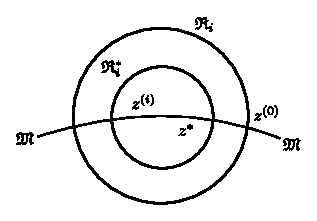
\includegraphics{figure3.eps}
\end{figure}

Let $\mathfrak{M}_{i}=\mathfrak{M}\cap \mathfrak{R}_{i}$. Consider now
the analytic set defined in the polycylinder $|w|<b$, $|t|\leq 2$ by
$Q(w,v^{\ast}t)=0$. Let $\mathfrak{B}$ be an irreducible component of
this analytic set, containing $(w^{\ast},1)$. Clearly if
$(w,t)\in\mathfrak{B}$, then $(w,v^{\ast}t)\in\mathfrak{M}_{i}$. On
$\mathfrak{B}$, therefore, we have after \eqref{187}, for the function
$f_{0}(w,v^{\ast}t)=f(z)$ that
$$
f^{\ast}(w,t)=f_{0}(w,v^{\ast}t)=t^{l}\sum^{g_{i}-1}_{v=0}t^{-1}b^{(i)}_{v}(v^{\ast}t)w^{v}. 
$$\pageoriginale
Since $b^{(i)}_{v}(v_{2},\ldots,v_{n})$ is of order at least $l$ in
$v_{2},\ldots,v_{n}$, it follows that $t^{-l}b^{(i)}_{v}(v^{\ast}t)$
is regular in $|t|\leq 2$. Hence $t^{-l}f^{\ast}(w,t)$ is regular on
$\mathfrak{B}$. Now it can be shown that if
$(w_{0},t_{0})\in\mathfrak{B}$, then $\mathfrak{B}$ can be
parametrized locally at $(w_{0},t_{0})$ by
$$
t-t_{0}=u^{q}, w-w_{0}=R(u),
$$
where $q$ is a positive integer and $R(u)$ is regular in $u$. If we
note that we can apply the maximum modulus principle to the function
$t^{-l}f^{\ast}(w,t)$ as a function of $u$, we can show that
$t^{-l}f^{\ast}(w,t)$ attains its maximum modulus on $\mathfrak{B}$ at
a point $(w^{(0)},t^{(0)})$ on the boundary of $\mathfrak{B}$ and
hence with $|t^{(0)}|=2$, necessarily. Thus
\begin{align*}
1=f(z^{\ast})=f_{0}(w^{\ast},v^{\ast}) &\leq
\Max\limits_{\mathfrak{B}}|t^{-l}f^{\ast}(w,t)|\\
&= 2^{-l}|f^{\ast}(w^{(0)},t^{(0)})|\\
&\leq 2^{-l}\Max\limits_{\substack{|t|\leq 2,|w|\leq
    b\\ (w,t)\in\mathfrak{B}}}|f^{\ast}(w,v^{\ast}t)|\tag{189}\label{189}\\
&\leq 2^{-l}\Max\limits_{\mathfrak{M}_{i}}|f(z)|.
\end{align*}


Let $z^{(0)}$ be a point on the boundary of $\mathfrak{M}_{i}$ at
which $\max\limits_{z\in\mathfrak{M}_{i}}|f(z)|$ is attained. If
$z^{(0)}\in\mathfrak{F}^{\ast}$, then $z^{(0)}\in\mathfrak{N}$ and
hence $|f(z^{(0)})|\leq 1$. Hence we have $1\leq 2^{-l}$, which gives
a contradiction, since $l\geq 1$. Therefore $f(z)$ must vanish on
$\mathfrak{N}$.

Suppose now $z^{(0)}\not\in \mathfrak{F}^{\ast}$. Then, for some
$M\in\Gamma$, we can ensure that $z^{(0)}_{M}\in\mathfrak{F}$.

We contend that there are only finitely many $P\in\Gamma$ for which
$\mathfrak{F}_{P}$ intersects
$\bigcup\limits^{c'}_{i=1}\mathfrak{R}_{i}$. To prove this, we first
apply Proposition \ref{prop23} with
$\bigcup\limits^{c'}_{i=1}\mathfrak{R}_{i}$ with $C$ and then for a
certain $b=b(C)>0$, we have $\mathfrak{U}_{\mu,b}\cap C=\emptyset$ for
all cusps $\mu$. It follows that for all cusps $\lambda$ and for all
$P\in\Gamma$, we have $(\mathfrak{U}_{\lambda,b})_{P}\cap
C=\emptyset$. In particular, for
$\lambda=\lambda_{1},\ldots,\lambda_{h}$, we see that
$(\mathfrak{U}_{\lambda,b})_{P}\cap C=\emptyset$,\pageoriginale for
all $P\in\Gamma$. Now
$\mathfrak{F}-\bigcup\limits^{h}_{i=1}\mathfrak{U}_{\lambda_{i},b}$ is
compact and we apply Proposition \ref{prop21} with
$\mathfrak{F}-\bigcup\limits^{h}_{i=1}\mathcal{U}_{\lambda_{i,b}}$ for $B$ and
$\bigcup\limits^{c'}_{i=1}\mathfrak{R}_{i}$ for $B'$. Then we see
immediately that our assertion above is true.

We may now suppose that
$z^{(0)}_{M}\in\mathfrak{F}\cap\mathfrak{U}_{\lambda_{1},c}$, without
loss of generality. Since
$z^{(0)}\in\bigcup\limits^{c'}_{i=1}\mathfrak{R}_{i}$, and since by
the remark above, $M=\left(\begin{smallmatrix} \alpha &\beta\\ \gamma
  & \delta\end{smallmatrix}\right)$ belongs to a finite set in
  $\Gamma$ independent of $z^{(0)}$, there exists a constant
  $c_{28}>1$ such that $|N(\gamma
  z^{(0)}+\delta)|>c^{-1}_{28}$. Further $|f(z^{(0)}_{M})||N(\gamma
  z^{(0)}+\delta)|^{-k}=|f(z^{(0)})|$. Hence from \eqref{189}, we have
$$
1\leq 2^{-l}|f(z^{(0)})|\leq 2^{-l}c^{k}_{28}|f(z^{(0)}_{M})|.
$$
If $z^{(0)}_{M}\in\mathfrak{F}^{\ast}$, then we have
$|f(z^{(0)}_{M})|\leq 1$ and therefore
$$
1\leq 2^{-l}c^{k}_{28}.
$$

Suppose now $z^{(0)}_{M}\not\in \mathfrak{F}^{\ast}$; then
$z^{(0)}_{M}\in\mathfrak{U}_{\lambda_{1},d'}\cap \mathfrak{F}$. We
shall show again that $|f(z^{(0)}_{M})|\leq 1$.

Let $\mathfrak{M}^{\ast}$ be the connected component of
$\mathfrak{M}\cap \mathfrak{U}_{\lambda_{1},d'}$ which contains the
point $z^{(0)}_{M}$. Then $f(z)$ is not locally constant on
$\mathfrak{M}^{\ast}$ near $z^{(0)}_{M}$, because of
$f(z^{(i)}_{M})=0$ and the connectedness of $\mathfrak{R}_{i}$.

Let $\sup\limits_{z\in\mathfrak{M}^{\ast}}|f(z)|=\delta$. If
$B=\bigcup\limits_{T\in\Gamma_{\lambda_{l}}}\mathfrak{M}^{\ast}_{T}$
  then clearly $\sup\limits_{z\in B}|f(z)|=\delta$, again. Now, since
  $f(z)$ tends to zero as $z$ tends to the cusp $\lambda_{1}$, there
  exists $d''$ with $0<d''<d'$ such that $|f(z)|<(1/2)\delta$ in
  $\mathfrak{U}_{\lambda_{1},d''}$. Let $B_{1}=B\cap
  (\ob{\mathfrak{U}}_{\lambda_{1}},d'-\mathfrak{U}_{l_{\lambda_{1}}},d'')\cap
  \mathfrak{F}$; then $B\cap
  (\ob{\mathfrak{U}}_{\lambda_{1},d'}-\mathfrak{U}_{\lambda_{1},d''})=\bigcup\limits_{T\in\Gamma_{\lambda_{1}}}(B_{1})_{T}$
  and further $\sup\limits_{z\in B_{1}}|f(z)|=\delta$, again. Since
  $\ob{B}_{1}$ is compact, $|f(z)|$ attains its maximum $\delta$
  ($<\infty$, necessarily therefore) at a point $z'$, say, in
  $\ob{B}_{i}$. Now, there exists a sequence of points
  $w^{(i)}\in\mathfrak{M}^{\ast}_{T_{i}}\cap \mathfrak{F}$ converging
  to $z'$. Using the fact that $\mathfrak{M}$ is closed and locally
  connected, it can be shown that $z'$ belongs already to
  $\ob{\mathfrak{M}^{\ast}_{T}}$ for a $T\in\Gamma_{\lambda_{1}}$,
  which is one of the $T_{i}$'s above. Now
  $|f((z^{(0)}_{M})_{T})|=|f(z^{(0)}_{M})|$ and to show that
  $|f(z^{(0)}_{M})|\leq 1$, we might as well argue with
  $\mathfrak{M}^{\ast}_{T}$ instead of $\mathfrak{M}^{\ast}$. Thus we
  may assume, without loss of generality, that $|f(z)|$ attains its
  maximum $\delta$ on $\ob{\mathfrak{M}^{\ast}}$ at a point $z'$. We
  now claim\pageoriginale that $\Delta(z',\lambda_{1})=d'$. For, if
  $\Delta(z',\lambda_{1})<d'$, then $z'\in\mathfrak{M}^{\ast}$ and we
  can find a curve $C$ in $\mathfrak{M}^{\ast}$ connecting
  $z^{(0)}_{M}$ with $z'$. Let $z''$ be the {\em first} point on $C$
  such that $|f(z'')|=\delta$; then $f(z)$ is not locally constant on
  $\mathfrak{M}^{\ast}$ near $z''$, and the maximum principle gives a
  contradiction. Thus $\Delta(z',\lambda_{1})=d'$. Again, for a
  suitable $T\in\Gamma_{\lambda_{1}}$, $z'_{T}\in\mathfrak{F}^{\ast}$
  \ie $z'_{T}\in\mathfrak{N}$, as before. Thus $|f(z^{(0)}_{M})|\leq
  |f(z')|=|f(z'_{R})|\leq 1$.

Thus, in all cases
$$
1\leq c^{k}_{28}2^{-l},
$$
\ie
$$
l\leq c_{29}k,
$$
if $f(z)$ does not vanish identically on $\mathfrak{N}$. But, from
this and from \eqref{188}, we obtain
$$
0<c_{30}l^{n}<c_{27}k^{n}\leq c_{26}(l+1)^{n-1}\leq c_{31}l^{n-1},
$$
\ie
$$
0<c_{30}<c_{27}\left(\frac{k}{l}\right)^{n}\leq \frac{c_{31}}{l}\leq
c_{31}.
$$
From the fact that $(k/l)^{n}$ is bounded, we see that as $k$ tends to
infinity, $l$ also tends to infinity. But this contradicts the
inequality $l<c_{31}/c_{30}$. Thus $f(z)$ vanishes on $\mathfrak{N}$
identically, for large $k$.

Now taking each $\mathfrak{R}_{i}$, $i=1,2,\ldots,c'$, we observe that
since $f(z)$ vanishes on the analytic set defined by $Q(z-z^{0})=0$ in
$\mathfrak{R}_{i}$, there exists an integer $n_{i}$ such that
$f^{n_{i}}(z)$ is divisible by $Q(z-z^{0})$ in $\mathfrak{R}_{i}$ \ie
$f^{n_{i}}(z)\varphi(z)$ is regular in $\mathfrak{R}_{i}$. (We might
take $n_{i}=g_{i}$, for example). Choosing $m=c_{26}$, we see that
$f^{m}(z)\varphi(z)$ is regular on $\mathfrak{F}^{\ast}$. Thus the
modular form $f^{m}(z)$ of weight $mk$ has the required property and
our lemma is therefore completely proved.

We are now, in a position, to prove (for $n\geq 2$), the main theorem,
viz.

\begin{thm}\label{thm19}
The Hilbert modular functions form an algebraic function field of $n$
variables. 
\end{thm}

\begin{proof}
We know by Proposition \ref{prop27} that there exist $n+1$ modular
forms\pageoriginale $f_{0}(z)$, $f_{1}(z),\ldots,f_{n}(z)$ of weight
$j$ such that
$\dfrac{f_{1}(z)}{f_{0}(z)},\ldots,\dfrac{f_{n}(z)}{f_{0}(z)}$ are
algebraically independent over the field of complex numbers. Since the
quotient of two modular forms of the same weight is a modular
function, we have $n$ algebraically independent modular functions
$$
g_{1}(z)=\dfrac{f_{1}(z)}{f_{0}(z)},\ldots,g_{n}(z)=\dfrac{f_{n}(z)}{f_{0}(z)}.
$$
\end{proof}

Let $\Omega$ denote the field of Hilbert modular functions and
$\Omega_{0}$, the field generated by $g_{1}(z),\ldots,g_{n}(z)$ over
the field of complex numbers. We shall first show that every element
of $\Omega$ satisfies a polynomial equation of bounded degree, with
coefficients in $\Omega_{0}$.

Let $\varphi(z)$ be any modular function. By the lemma above,
$\varphi(z)=\psi(z)/\chi(z)$, where $\chi(z)$ and $\psi(z)$ are two
modular forms of the same weight $k$. Let us consider for fixed
positive rational integers $m$ and $s$, the power products
$$
f_{k_{1},\ldots,k_{n},l}(z)=g^{k_{1}}_{1}(z),\ldots,g^{k_{n}}_{n}(z)\varphi^{l}(z),
\begin{cases}
k_{i}=0,1,2,\ldots,m,\\
l=0,1,2,\ldots,s.
\end{cases}
$$
Now $f_{0}^{mn}(z)\chi^{s}(z)f_{k_{1},\ldots,k_{n},l}(z)$ is a modular
  form of weight $w=mnj+ks$. We have indeed $(m+1)^{n}(s+1)$ such
  modular forms of weight $w$. If we can choose $m$ and $s$ such that
\begin{equation*}
(m+1)^{n}(s+1)>c_{20}w^{n}(\geq t(w)),\tag{190}\label{190}
\end{equation*}
then we get a nontrivial linear relation between these modular forms
and hence between the $(m+1)^{n}(s+1)$ functions
$f_{k_{1},\ldots,k_{n},l}(z)$. But this linear relation cannot be
totally devoid of terms involving powers of $\varphi(z)$, since
otherwise, this will contradict the algebraic independence of
$g_{1}(z),\ldots,g_{n}(z)$. Thus $\varphi(z)$ satisfies a polynomial
equation of degree at most $s$ and with coefficients in
$\Omega_{0}$. Since $\Omega$ is a separable algebraic extension of
$\Omega_{0}$ and since every element of $\Omega$ satisfies a
polynomial equation of degree at most $s$ over $\Omega_{0}$, it
follows that $\Omega$ is a finite algebraic extension of $\Omega_{0}$
\ie an algebraic function field of $n$ variables.

In order to complete the proof of the theorem, we have only to find
rational integers $\ub{m}$ and $\ub{s}$ which satisfy \eqref{190}, $s$
being bounded. This is very\pageoriginale simple, for when $m$ tends
to infinity, $\dfrac{w^{n}}{(m+1)^{n}}$ tends to $(jn)^{n}$ so that if
we choose $m$ large enough and $s>c_{20}j^{n}n^{n}$, then \eqref{190}
will be fulfilled. Our theorem is therefore completely proved.

By adopting methods similar to the above, Siegel has recently\break proved
that (for $n\geq 2$) every modular function of degree $n$ (\ie\ a
complex-valued function meromorphic in the Siegel half-plane and
invariant under the modular transformations) can be expressed as the
quotient of two ``entire'' modular forms of degree $n$. (See reference
(32), Siegel). It had been already shown by Siegel that the modular
functions of degree $n$ which are quotients of ``entire'' modular
forms, form an algebraic function field of $n(n+1)/2$ variables.

\begin{thebibliography}{99}
\bibitem{c3:key1} \textsc{A.\@ A.\@ Albert:} A solution of the principal
  problem in the theory of Riemann matrices, {\em Ann.\@ of Math.,} 35
  (1934), 500-515.

\bibitem{c3:key2} \textsc{O.\@ Blumenthal:} \"Uber Modulfunktionen von
  mehreren Ver\"anderlichen, {\em Math.\@ Ann.,} 56 (1903), 509-548;
  ibid 58 (1904), 497-527.

\bibitem{c3:key3} \textsc{L.\@ R.\@ Ford:} {\em Automorphic functions,}
  Chelsea, New York (1951).

\bibitem{c3:key4} \textsc{F.\@ G\"otzky:} \"Uber eine zahlentheoretische
  Anwendung von Modulfunktionen zweier Ver\"anderlicher, {\em Math.\@
    Ann.} 100 (1928), 411-437.

\bibitem{c3:key5} \textsc{K.\@ B.\@ Gundlach:} \"Uber die Darstellung der
  ganzen Spitzenformen zu den Idealstufen der Hilbertschen Modulgruppe
  und die Absch\"atzung ihrer Fourierkoeffizienten, {\em Acta.\@
    Math.} 92 (1954), 309-345.

\bibitem{c3:key6} ------: Poincaresche und Eisensteinsche Reihen Zur
  Hilbertschen Modulgruppe, {\em Math.\@ Zeit.} 64 (1956), 339-352.

\bibitem{c3:key7} ------: Modulfunktionen zur Hilbertschen Modulgruppe und
  ihre Darstellung als Quotienten ganzer Modulformen, {\em Arch.\@
    Math.} 7 (1956), 333-338.

\bibitem{c3:key8} ------: \"Uber den Rang der Schar der ganzen automorphen
  Formen zu hyperabelschen Transformationsgruppen in zwei Variablen,
  {\em G\"ott.\@ Nachr.} Nr.\@ 3. (1958).

\bibitem{c3:key9} ------:\pageoriginale Quotientenraum und meromorphe Funktionen zur
  Hilbertschen Modulgruppe, {\em G\"ott.\@ Nachr.\@} Nr.\@ 3, (1960).

\bibitem{c3:key10} \textsc{E.\@ Hecke:} Grundlagen einer Theorie der
  Integralgruppen und der Integralperioden bei den Normalteilern der
  Modulgruppe, {\em Math.\@ Werke,} G\"ottingen, (1959), 731-772.

\bibitem{c3:key11} \textsc{L.\@ Hua:} On the theory of Fuchsian functions of
  several variables, {\em Ann.\@ of Math.,} 47 (1946), 167-191.

\bibitem{c3:key12} \textsc{H.\@ D.\@ Kloosterman:} Theorie der
  Eisensteinschen Reihen von mehreren Ver\"anderlichen, {\em Abh.\@
    Math.\@ Sem\@ Hamb.\@ Univ.} 6 (1928), 163-188.

\bibitem{c3:key13} \textsc{M.\@ Moecher:} Zur Theorie der Modulformen
  $n$-ten Grades I, {\em Math.\@ Zeit.} 59 (1954), 399-416.

\bibitem{c3:key14} \textsc{S.\@ Lefschetz:} On certain numerical invariants
  of algebraic varieties with applications to Abelian varieties, {\em
    Trans.\@ Amer.\@ Math.\@ Soc.,} 22 (1921), 327-482.

\bibitem{c3:key15} \textsc{H.\@ Maass:} \"Uber Gruppen von hyperabelschen
  Transformationen, {\em Sitz-Ber.\@ der Heidelb.\@ Akad.\@ der Wiss.,
    math.-nat.} K1.\@ 2 Abh. (1940).

\bibitem{c3:key16} -----: Zur Theorie der automorphen Funktionen von n
  Ver\"anderlichen, {\em Math.\@ Ann.,} 117 (1940), 538-578.

\bibitem{c3:key17} ------: Theorie der Poincar\'eschen Riehen zu den
  hyperbolischen Fixpunktsystemem der Hilbertschen Modulgruppe, {\em
    Math.\@ Ann.} 118 (1941), 518-543.

\bibitem{c3:key18} \textsc{H.\@ Petersson:} Einheitliche Begr\"undung der
  Vollst\"andigkeitss\"atze f\"ur die Poincar\'eschen Reihen von
  reeler Dimension bei beliebigen Grenzkreisgruppen von erster {\em
    Art, Abh.\@ Math.\@ Sem.\@ Hamb.\@ Univ.} 14 (1941), 22-60.

\bibitem{c3:key19} ------: \"Uber die Berechnung der Skalarprodukte ganzer
  Modulformen, Comment.\@ Math.\@ Helv. 22 (1949), 168-199.

\bibitem{c3:key20} \textsc{E.\@ Picard:} Sur les fonctions
  hyperab\'eliennes, {\em J.\@ de Liouville,} Ser.\@ IV, 1 (1885).

\bibitem{c3:key21} \textsc{H.\@ Poincar\'e:} Sur les fonctions fuchsiennes,
  {\em Oeuvres,} II, 169-257.

\bibitem{c3:key22} ------: Fonctions modularies et fonctions fuchsiennes,
  {\em Oeuvres,} II, 592-618.

\bibitem{c3:key23} \textsc{R.\@ A.\@ Rankin:} The scalar product of modular
  forms, {\em Proc.\@ Lond.\@ Math.\@ Soc.} 3, II (1952), 198-217.

\bibitem{c3:key24} \textsc{C.\@ Rosati:}\pageoriginale Sulle matrici di Riemann, {\em
  Rendiconti del Circ.\@ Mathematico di Palermo,} 53 (1929), 79-134.

\bibitem{c3:key25} \textsc{A. Selberg:} Beweis eines Darstellungssatzes aus
  der Theorie der ganzen Modulformen, {\em Arch.\@ for Math.}
  Naturvid. 44, Nr.\@ 3 (1940).

\bibitem{c3:key26} \textsc{I.\@ I.\@ Piatetskii-Shapiro:} Singular modular
  functions, {\em Izv.\@ Akad.\@ Nauk SSSR, Ser.\@ Mat.} 20 (1956), 53-98.

\bibitem{c3:key27} \textsc{C.\@ L.\@ Siegel:} \"Uber die analytische Theorie
  der quadratischen Formen, III, {\em Ann.\@ of Math.} 38 (1937), 213-292.

\bibitem{c3:key28} ------: Einf\"uhrung in die Theorie der Modulfunktionen
  $n$-ten Grades, {\em Math.\@ Ann.} 116 (1939), 617-657.

\bibitem{c3:key29} ------: Die Modulgruppe in einer einfachen
  involutorischen Algebra, {\em Festschrift Akad.\@ Wiss.}
  G\"ottingen, 1951.

\bibitem{c3:key30} ------: {\em Automorphe Funktionen in mehreren
  Variablen,} G\"ottingen, (Function theory in 3 Volumes) (1954-55).

\bibitem{c3:key31} ------: Zur Vorgeschichte des Eulerschen
  Additons-theorem, Sammelband Leonhard Euler, {\em Akad.\@ Verlag,}
  Berlin, (1959), 315-317.

\bibitem{c3:key32} ------: \"Uber die algebraische Abh\"angigkeit von
  Modulfunktionen $n$-ten Grades, {\em G\"ott.\@ Nacher.} Nr.\@ 12, (1960).

\bibitem{c3:key33} \textsc{H.\@ Weyl:} On generalized Riemann matrices, {\em
  Ann.\@ of Math.} 35 (1934), 714-729.
\end{thebibliography}
